% Aberdeen style guide should be followed when using this
% layout. Their template powerpoint slide is used to extract the
% Aberdeen color and logo but is otherwise ignored (it has little or
% no formatting in it anyway).
%
% http://www.abdn.ac.uk/documents/style-guide.pdf

%%%%%%%%%%%%%%%%%%%% Document Class Settings %%%%%%%%%%%%%%%%%%%%%%%%%
% Pick if you want slides, or draft slides (no animations)
%%%%%%%%%%%%%%%%%%%%%%%%%%%%%%%%%%%%%%%%%%%%%%%%%%%%%%%%%%%%%%%%%%%%%%
%Normal document mode
\documentclass[10pt,compress]{beamer}
%Draft or handout mode
%\documentclass[10pt,compress,handout]{beamer}
%\documentclass[10pt,compress,handout,ignorenonframetext]{beamer}
\newcommand{\frc}{\displaystyle\frac}


%%%%%%%%%%%%%%%%%%%% General Document settings %%%%%%%%%%%%%%%%%%%%%%%
% These settings must be set for each presentation
%%%%%%%%%%%%%%%%%%%%%%%%%%%%%%%%%%%%%%%%%%%%%%%%%%%%%%%%%%%%%%%%%%%%%%

\newcommand{\shortname}{Dr Jeff Gomes}
\newcommand{\fullname}{Dr Jeff Gomes}
\institute{School of Engineering}
\newcommand{\emailaddress}{jefferson.gomes@abdn.ac.uk}
\newcommand{\logoimage}{../FigBanner/UoAHorizBanner}
\title{Engineering Thermodynamics (EG3521)}
\subtitle{Module 3: Refrigeration $\&$ Liquefaction}
\date[04-11/03/2014]{04-11 March 2014}


%%%%%%%%%%%%%%%%%%%% Template settings %%%%%%%%%%%%%%%%%%%%%%%%%%%%%%%
% You shouldn't have to change below this line, unless you want to.
%%%%%%%%%%%%%%%%%%%%%%%%%%%%%%%%%%%%%%%%%%%%%%%%%%%%%%%%%%%%%%%%%%%%%%
\usecolortheme{whale}
\useoutertheme{infolines}

% Use the fading effect for items that are covered on the current
% slide.
\beamertemplatetransparentcovered

% We abuse the author command to place all of the slide information on
% the title page.
\author[\shortname]{%
  \fullname\\\ttfamily{\emailaddress}
}


%At the start of every section, put a slide indicating the contents of the current section.
%\AtBeginSection[] {
%  \begin{frame}
%    \frametitle{Section Outline}
%    \tableofcontents[currentsection]
%  \end{frame}
%}

% Allow the inclusion of movies into the Presentation! At present,
% only the Okular program is capable of playing the movies *IN* the
% presentation.
\usepackage{multimedia}
\usepackage{animate}

%%%%% Color settings
\usepackage{color}
%% The background color for code listings (i.e. example programs)
\definecolor{lbcolor}{rgb}{0.9,0.9,0.9}%
\definecolor{UoARed}{rgb}{0.64706, 0.0, 0.12941}
\definecolor{UoALight}{rgb}{0.85, 0.85, 0.85}
\definecolor{UoALighter}{rgb}{0.92, 0.92, 0.92}
\setbeamercolor{structure}{fg=UoARed} % General background and higlight color
\setbeamercolor{frametitle}{bg=black} % General color
\setbeamercolor{frametitle right}{bg=black} % General color
\setbeamercolor{block body}{bg=UoALighter} % For blocks
\setbeamercolor{structure}{bg=UoALight} % For blocks
% Rounded boxes for blocks
\setbeamertemplate{blocks}[rounded]

%%%%% Font settings
% Aberdeen requires the use of Arial in slides. We can use the
% Helvetica font as its widely available like so
% \usepackage{helvet}
% \renewcommand{\familydefault}{\sfdefault}
% But beamer already uses a sans font, so we will stick with that.

% The size of the font used for the code listings.
\newcommand{\goodsize}{\fontsize{6}{7}\selectfont}

% Extra math packages, symbols and colors. If you're using Latex you
% must be using it for formatting the math!
\usepackage{amscd,amssymb} \usepackage{amsfonts}
\usepackage[mathscr]{eucal} \usepackage{mathrsfs}
\usepackage{latexsym} \usepackage{amsmath} \usepackage{bm}
\usepackage{amsthm} \usepackage{textcomp} \usepackage{eurosym}
% This package provides \cancel{a} and \cancelto{a}{b} to "cancel"
% expressions in math.
\usepackage{cancel}

% Get rid of font warnings as modern LaTaX installations have scalable
% fonts
\usepackage{type1cm} 

%\usepackage{enumitem} % continuous numbering throughout enumerate commands

% For exact placement of images/text on the cover page
\usepackage[absolute]{textpos}
\setlength{\TPHorizModule}{1mm}%sets the textpos unit
\setlength{\TPVertModule}{\TPHorizModule} 

% Source code formatting package
\usepackage{listings}%
\lstset{ backgroundcolor=\color{lbcolor}, tabsize=4,
  numberstyle=\tiny, rulecolor=, language=C++, basicstyle=\goodsize,
  upquote=true, aboveskip={1.5\baselineskip}, columns=fixed,
  showstringspaces=false, extendedchars=true, breaklines=false,
  prebreak = \raisebox{0ex}[0ex][0ex]{\ensuremath{\hookleftarrow}},
  frame=single, showtabs=false, showspaces=false,
  showstringspaces=false, identifierstyle=\ttfamily,
  keywordstyle=\color[rgb]{0,0,1},
  commentstyle=\color[rgb]{0.133,0.545,0.133},
  stringstyle=\color[rgb]{0.627,0.126,0.941}}

% Allows the inclusion of other PDF's into the final PDF. Great for
% attaching tutorial sheets etc.
\usepackage{pdfpages}
\setbeamercolor{background canvas}{bg=}  

% Remove foot note horizontal rules, they occupy too much space on the slide
\renewcommand{\footnoterule}{}

% Force the driver to fix the colors on PDF's which include mixed
% colorspaces and transparency.
\pdfpageattr {/Group << /S /Transparency /I true /CS /DeviceRGB>>}

% Include a graphics, reserve space for it but
% show it on the next frame.
% Parameters:
% #1 Which slide you want it on
% #2 Previous slides
% #3 Options to \includegraphics (optional)
% #4 Name of graphic
\newcommand{\reserveandshow}[4]{%
\phantom{\includegraphics<#2|handout:0>[#3]{#4}}%
\includegraphics<#1>[#3]{#4}%
}

\begin{document}

% Title page layout
\begin{frame}
  \titlepage
  \vfill%
  \begin{center}
    \includegraphics[clip,width=0.8\textwidth]{\logoimage}
  \end{center}
\end{frame}

% Table of contents
%\frame{ \frametitle{Slides Outline}
%  \tableofcontents
%}


%%%%%%%%%%%%%%%%%%%% The Presentation Proper %%%%%%%%%%%%%%%%%%%%%%%%%
% Fill below this line with \begin{frame} commands! It's best to
% always add the fragile option in case you're going to use the
% verbatim environment.
%%%%%%%%%%%%%%%%%%%%%%%%%%%%%%%%%%%%%%%%%%%%%%%%%%%%%%%%%%%%%%%%%%%%%%



\section{Gas Refrigeration Cycles}
\subsection{Previously in EG3521 ...}
%%%
%%% Slides
%%%
\begin{frame}
 \frametitle{Bell-Coleman Cycle (or Reversed Brayton Cycle)}
    \begin{figure}%
     \begin{center}
      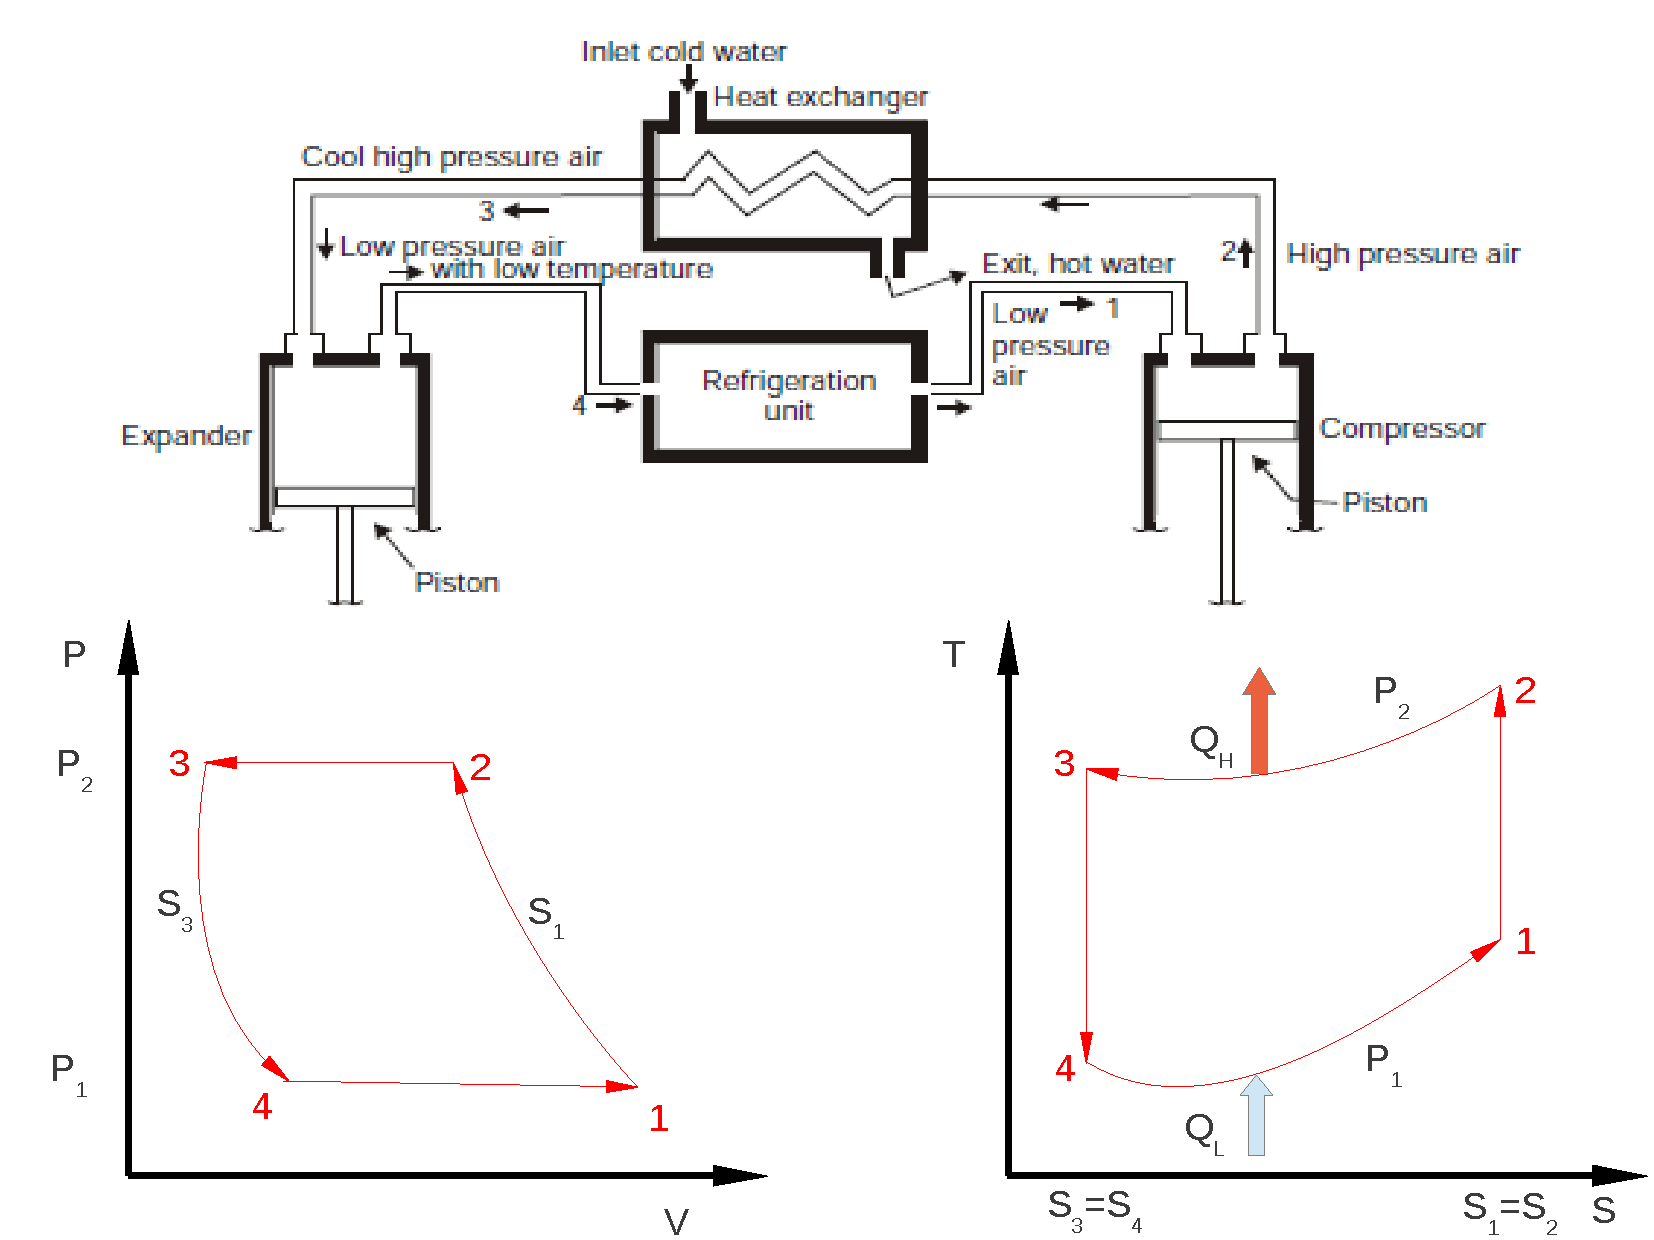
\includegraphics[width=8.3cm,height=7.6cm]{./Pics/Overview_Refrig6}
     \end{center}
    \end{figure}  
\end{frame}
%%%
%%% Slides
%%%
\begin{frame}
 \frametitle{Comparison between Gas-Refrigeration Cycles}

    \begin{figure}%
     \begin{center}
      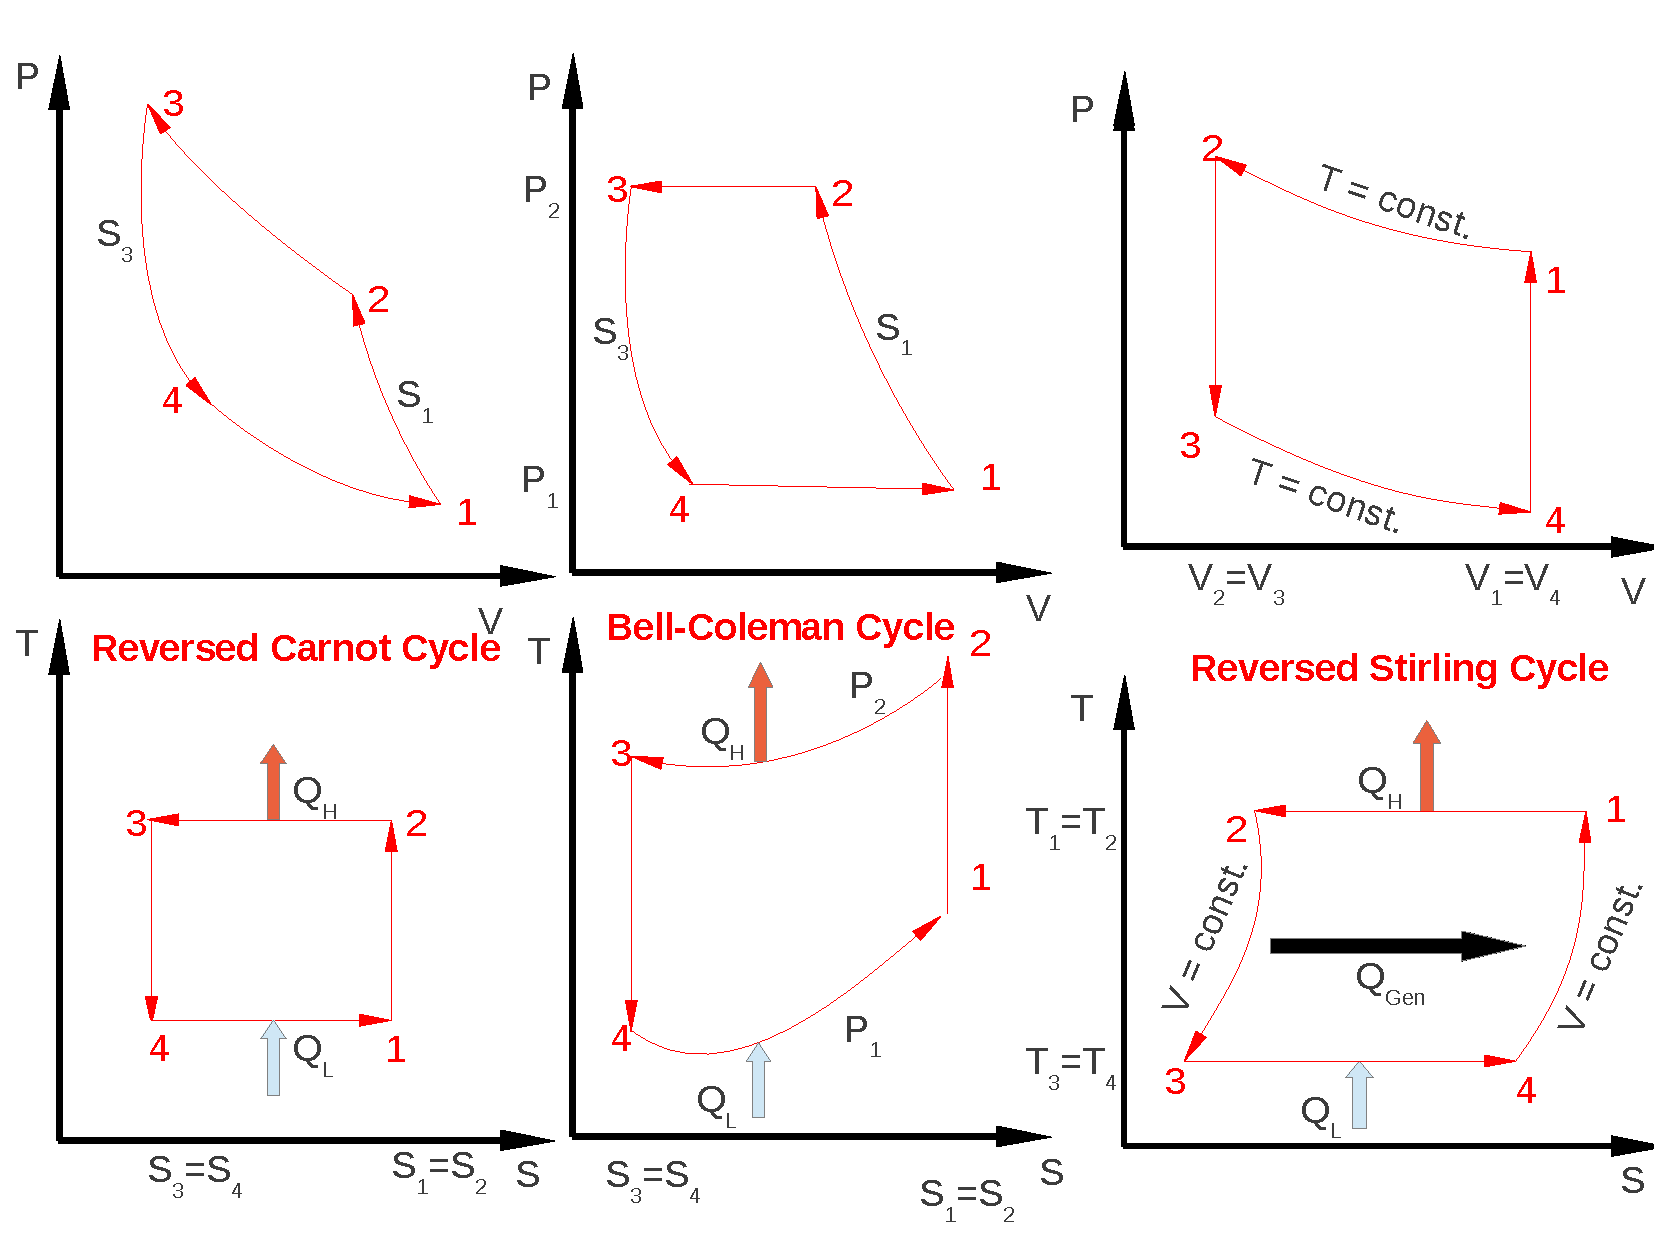
\includegraphics[width=11.5cm,height=7.8cm]{./Pics/Overview_Refrig10}
     \end{center}
    \end{figure}  

\end{frame}

%%%
%%%  SECTION
%%%
\section{Vapour Refrigeration Cycles}

\subsection{Motivation}
%%%
%%% Slide
%%%
\begin{frame}
 \frametitle{Introduction}
  In Module 4, we will cover the following topics:
  \begin{enumerate}[(i)]
   \item <1-> Fundamentals of Refrigeration: Refrigeration and heat pump; Elements of refrigeration; Efficieny; Classification and Properties of Refrigerants;
   \item <1-> Gas-Refrigeration Systems: Reversed Carnot, Brayton and Stirling cycles;
   \item <1-> Analysis of Air-Conditioning Processes and;
   \item <2-> \textcolor{blue}{Vapour-Refrigeration Systems: Ideal and Actual Vapour-Compression Refrigeration Cycles; Criteria for choosing Refrigerant Fluids; Cascade and Multi-stage Vapour-Compression systems;}
   \item <3-> \textcolor{blue}{Absorption Refrigeration Systems;}
   \item <3-> \textcolor{blue}{Liquefaction Processes: Claude and Linde Cycles.}
  \end{enumerate}
\end{frame}

\subsection{Intended Learning Objectives}
%%%
%%% Slide
%%%
\begin{frame}
 \frametitle{Aims and Objectives}
  At the end of this Module, you should be able to:
  \begin{enumerate}[(i)]
   \item <1-> Identify elements of vapour-compression refrigeration cycles;
   \item <2-> Identify refrigerant fluids and their properties;
   \item <3-> Solve problems based on the reversed Rankine cycle;
   \item <4-> Identify simplifying assumptions for second-law analysis of vapour-refrigeration cycles.
  \end{enumerate}
\end{frame}


\subsection{Bibliography} 
%%%
%%% Slide
%%%
\begin{frame}
 \frametitle{Suggested References}
  Literature relevant for this module:
  \begin{enumerate}[(a)]
   \item J.M. Smith, H.C. Van Ness and M.M. Abbott, $\lq$Introduction to Chemical Engineering Thermodynamics', 6$^{th}$ Edition: Chapter 9.2;
   \item I. Muller and W.H. Muller, $\lq$Fundamentals of Thermodynamics and Applications' (2009) Chapter 6.3;
   \item Y.A. Cengel and M.A. Boles, $\lq$Thermodynamics -- An Engineering Approach' , 5$^{th}$ Edition: Chapters 11.3-5,7;
   \item E. Logan, $\lq$Thermodynamics -- Processes and Applications' (1999): 8.2-3;
   \item M.J. Moran, H.J. Shapiro, D.D. Boettner, M.B. Bailey, $\lq$Principles of Engineering Thermodynamics', 7$^{th}$ Edition: Chapters: 10.1-4;
   \item R.T. Balmer, $\lq$Modern Engineering Thermodynamics' (2011) Chapters: 14.2,5-9;
   \item \href{http://www.sfsb.unios.hr/test/testhome/vtAnimations/animations/chapter09/refrigeration/index1.html}{\tiny{http://www.sfsb.unios.hr/test/testhome/vtAnimations/animations/chapter09/refrigeration/index1.html}}
  \end{enumerate}
\end{frame}


\subsection{Fluid Refrigerants}
%%%
%%% Slide
%%%
\begin{frame}
 \frametitle{Definition of Refrigerants}
  \begin{enumerate}[(a)]
   \item <1-> \textcolor{blue}{Refrigerant} is the working fluid used in refrigeration equipment; 
   \item <2-> Its main function is to \textcolor{blue}{carry/reject heat} as \textcolor{blue}{sensible heat} (i.e., heat transfer with change in temperature) or \textcolor{blue}{latent heat} (i.e., heat transfer with no change in temperature -- during phase change);
   \item <3-> In other words, refrigerant fluids act as cooling agents by absorbing heat from a body or substance;
   \item <4-> During vapour-compression refrigeration cycles, the working fluid vaporises and condenses as it absorbs and releases heat;
   \item <5-> Therefore any \textcolor{blue}{volatile fluid} that is liquid at the required temperature in the evaporator can be effectively used as refrigerant. However the following are characteristics required by a fluid for a given refrigeration process:
  \end{enumerate}
\end{frame}

%%%
%%% Slide
%%%
\begin{frame}
 \frametitle{Characteristics of Refrigerants -- A few important criteria}
 \begin{enumerate}[(a)]
   \item <1-> Low boiling and fusion (or freezing) temperatures at atmospheric pressure. Here, we want to supply the minimum work in the compressor (low $T_{b}$) and avoid any freezing (T$_{f}$) in the compressor; 
   \item <2-> Critical temperature should be higher than the condenser temperature for the ease condensation;
   \item <3-> High latent heat $\Longrightarrow$ high refrigerant effect per unit mass of refrigerant circulated;
   \item <4-> Small specific volume at the inlet of the compressor $\Longrightarrow$ reduction of the compressor size for the same refrigeration capacity;
   \item <5-> Small $C_{p,l}$ and Large $C_{p,v}$ $\Longrightarrow$ increases the refrigerating capacity per unit mass of refrigerant;
   \item <6-> Large Thermal conductivity;
   \item <7-> Small viscosity $\Longrightarrow$ leads to better heat transfer and small pumping work requirement;
   \item <8-> Safe (toxicity and flammability) and Compatible with the materials that it will be in contact with (i.e., chemically inert);
   \item <10-> Low cost and widely available;
   \item <11-> Environmental compatible.
  \end{enumerate}
\end{frame}

%%%
%%% Slide
%%%
\begin{frame}
 \frametitle{Classification of Refrigerants}
 \begin{enumerate}[(a)]
   \item <1-> \textcolor{blue}{Primary Refrigerants} (PR) are directly involved in refrigeration systems and is usually followed by a \textcolor{blue}{phase change}. The cycle encompass compression, condensation, expansion and evaporation;
   \item <2-> \textcolor{blue}{Secondary Refrigerants} (SR) is used as a heat transfer medium  \textcolor{blue}{without phase change} but \textcolor{blue}{with change in temperature};
   \item <3-> As an example, in a conventional air conditioning system, there are 2 cycles: 
    \begin{enumerate}[(i)]
     \item <4-> \textcolor{blue}{Water} is the \textcolor{blue}{{\it primary refrigerant}} that circulates throughout the closed-loop cycle involving evaporator, compressor, condenser and expansion valve, whereas;
     \item <5-> \textcolor{blue}{Air} is the \textcolor{blue}{{\it secondary refrigerant}}.
    \end{enumerate}
    \item <6-> PR are used in vapour-compression systems whereas SR are liquids used for transporting low-temperature heat energy (e.g., brine, anti-freezing agents etc);
  \end{enumerate}
\end{frame}

%%%
%%% Slide
%%%
\begin{frame}
 \frametitle{Classification of Refrigerants -- PR}
%\textcolor{blue}{\bf PR} can be further classified into 4 categories depending upon their characteristics: 
 \begin{enumerate}[(a)]
   \item <1-> \textcolor{red}{Halocarbon Compounds:} contains 1 or more halogens {\it (Cl, F and Br)}. Commonly traded under the brand names of {\it Freon, Genetron etc} under the family of CFCs (chloro fluoro carbons) -- 1940-1990. Hydrogen has replaced chlorine and make this class of refrigerants more $\lq$environmental friendly' with a designation HFC (hydrofluiro carbons -- HFC). All halocarbon refrigerants are named as {\it R-XYZ}, e.g., {\it R-22} (monochloro difluoro-methane), {\it R-114} (dichloro tetrafluoro-ethane); 
   \item <2-> \textcolor{red}{Inorganic Compounds:} e.g., ammonia ({\it R-117}), CO$_{2}$ ({\it R-744}), SO$_{2}$ ({\it R-764}), water ({\it R-718}), etc;
   \item <3-> \textcolor{red}{Hydrocarbons} are often in the petroleum and petrochemical industry in liquefaction of gases, e.g., methane ({\it R-50}), propane ({\it R-290}), etc;
   \item <4-> \textcolor{red}{Azeotropes} are mixtures of 2 or more substances that behave as if they are compounds. This is because they can not be separated into their individual components by distillation. An azeotrope substance evaporates and condenses as a single substance with properties that are intrinsically different from the original constituents. E.g., {\it R-500}: 74$\%$ of {\it R-12} and 26$\%$ of {\it R-115}, etc;
   \item <5-> \textcolor{red}{Unsaturated Organic Compounds} are hydrocarbons based on ethylene and propylene. E.g., Trichloro ethylene ({\it R-1120}), Propylene ({\it R-1270}), etc.
 \end{enumerate}
\end{frame}

%%%
%%% Slide
%%%
\begin{frame}
 \frametitle{Classification of Refrigerants -- SR}
 \begin{enumerate}[(a)]
   \item <1-> SR are indirect refrigerants that transfer heat from the substance that need to be cooled to the evaporator; 
   \item <2-> Change in temperature are due to the absorption of heat followed by rejection in the evaporator with \textcolor{blue}{{\bf no} phase change};
   \item <3-> SR fluids commonly found in industrial and domestic applications are water, brine, anti-freezing (solution of water and ethylene glycol, propylene glycol, calcium chloride etc).
 \end{enumerate}
\end{frame}




\subsection{Vapour-Compression Refrigeration Cycle}
%%%
%%% Slide
%%%
\begin{frame}
 \frametitle{Introduction}
  \begin{columns}
   \begin{column}[c]{0.5\linewidth}
    \begin{figure}%
     \begin{center}
      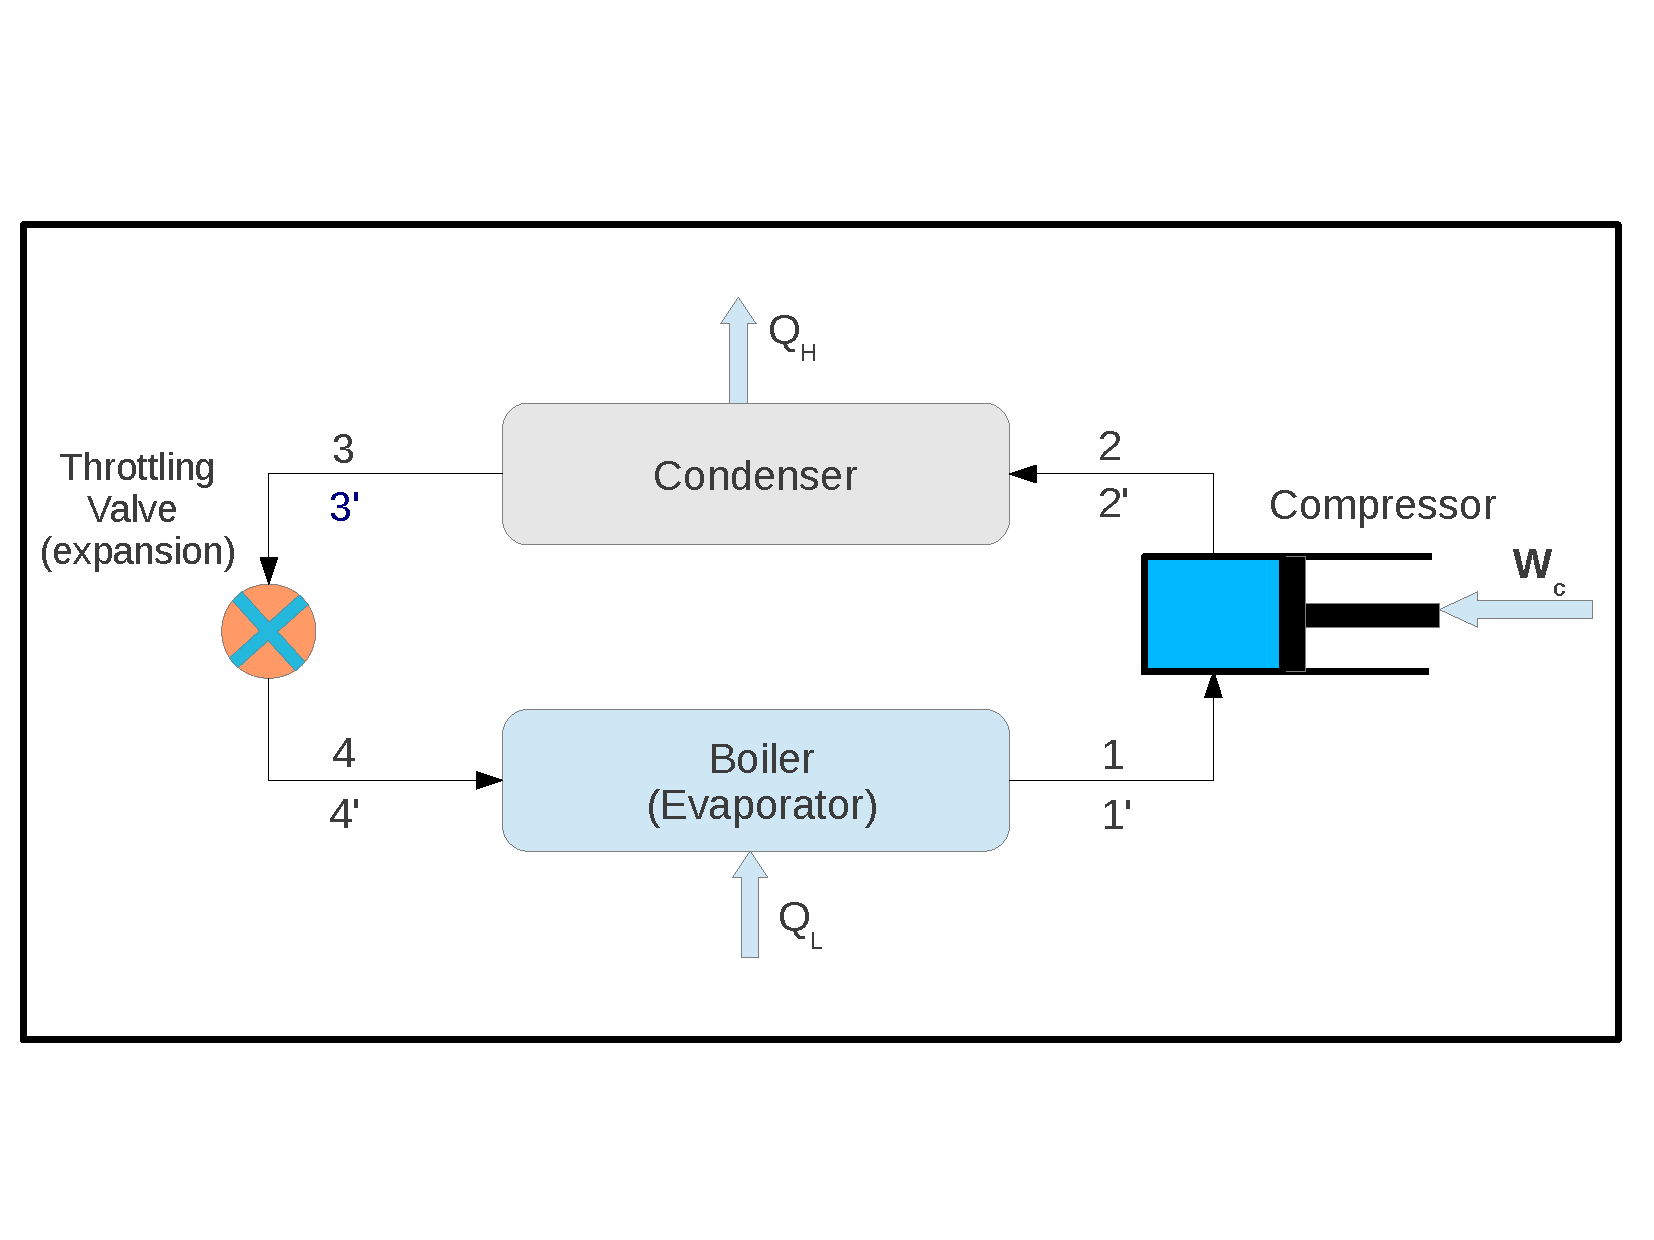
\includegraphics[width=5.8cm,clip]{./Pics/Overview_Refrig12}
     \end{center}
    \end{figure}  
   \end{column}  
   \begin{column}[c]{0.5\linewidth}
  \begin{enumerate}[(a)]
   \item <1-> First vapour-compression refrigeration system was a closed system introduced by Jacob Perkins (1766-1849) using \textcolor{blue}{diethyl ether} as refrigerant fluid;
   \item <2-> Ether vapour was compressed in a piston-cylinder system and condensed (i.e., turned into liquid) at a higher saturation pressure and temperature;
   \item <3-> Liquid ether is throttled through a valve back into the low-pressure evaporator;
   \item <4-> This process takes place beneath the vapour dome of the ether and it is a \textcolor{blue}{reversed Rankine cycle}.
  \end{enumerate}
 \end{column}  
\end{columns}
\end{frame}


%%%
%%% Slide
%%%
\begin{frame}
 \frametitle{Introduction}

  A few animations for reversed Brayton, Rankine cycles can be found in:
\href{http://www.sfsb.unios.hr/test/testhome/vtAnimations/animations/chapter09/refrigeration/index1.html}{\tiny{http://www.sfsb.unios.hr/test/testhome/vtAnimations/animations/chapter09/refrigeration/index1.html}}


\end{frame}


%%%
%%% Slide
%%%
\begin{frame}
 \frametitle{Description of the Cycle}
  \begin{columns}
   \begin{column}[c]{0.55\linewidth}
    \begin{figure}%
     \vbox{
      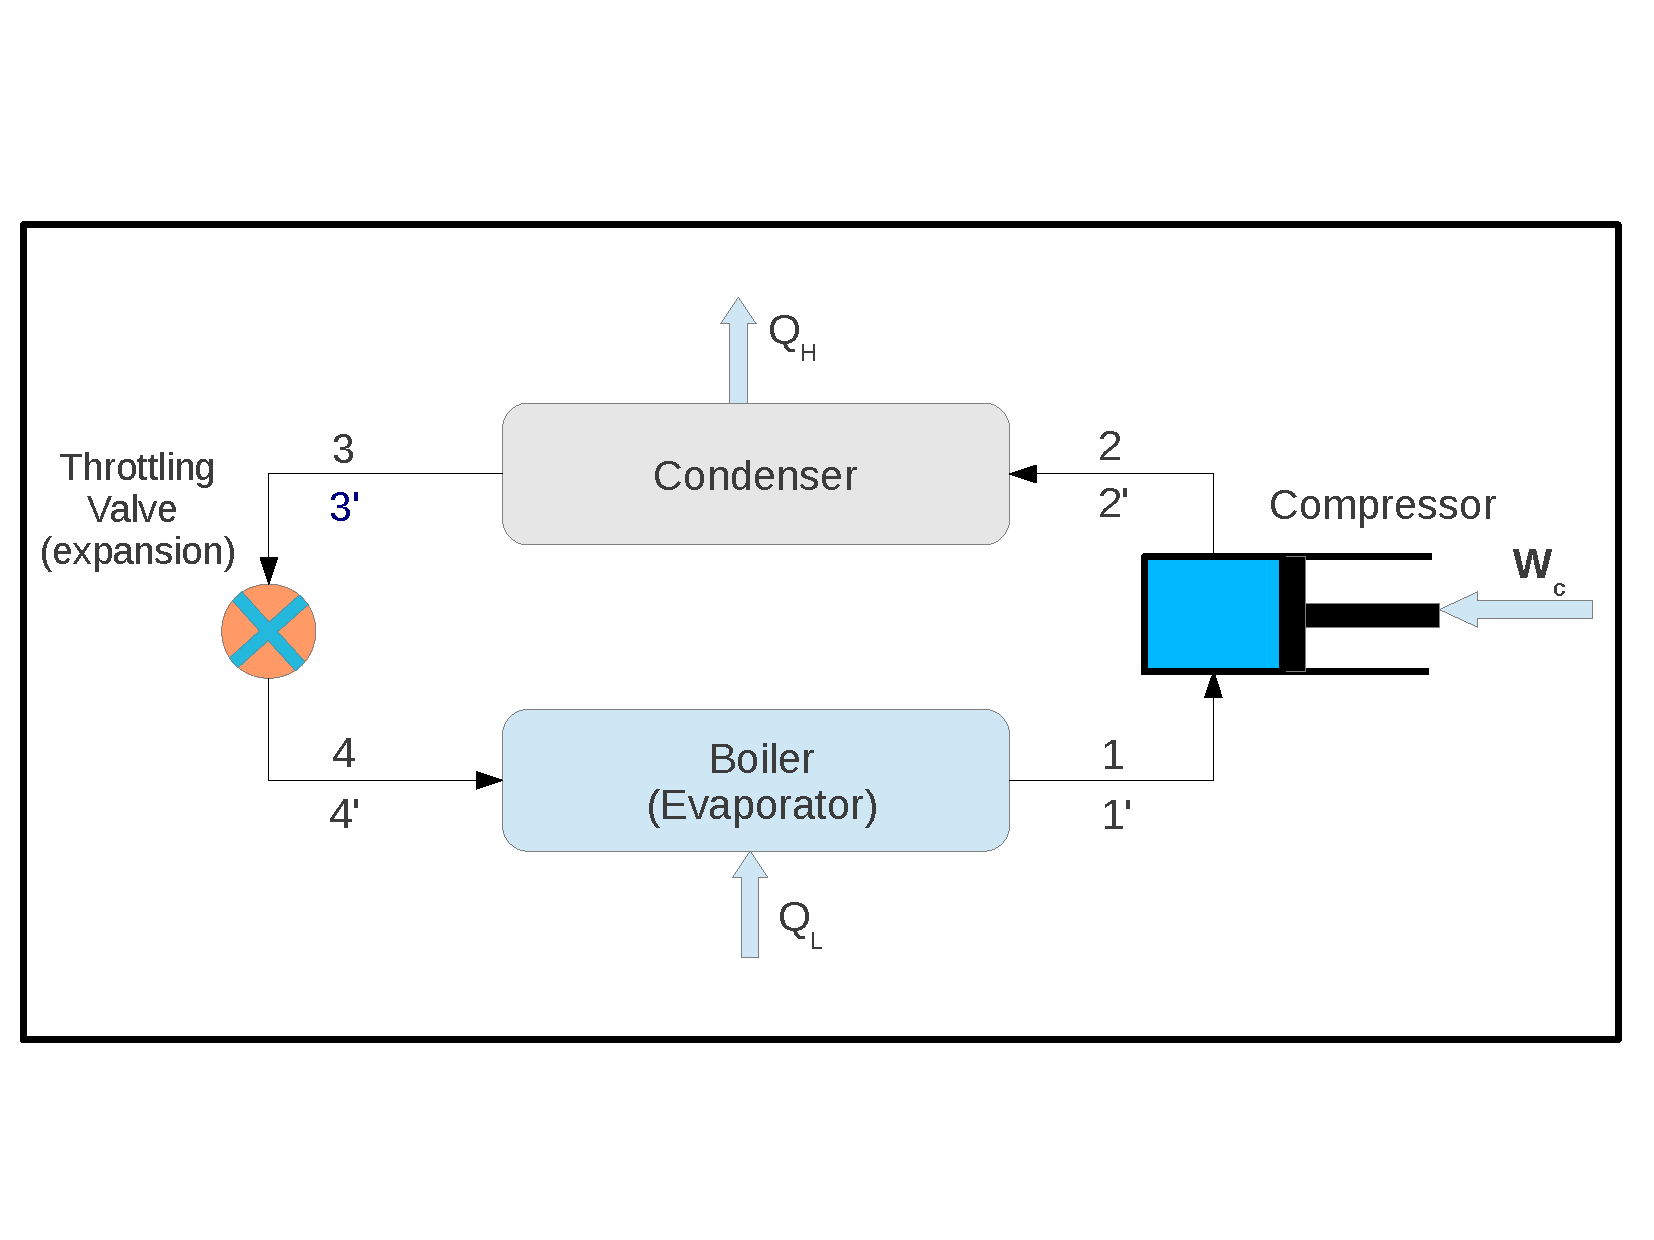
\includegraphics[width=5.5cm,clip]{./Pics/Overview_Refrig12}
      \vspace{-.5cm}
      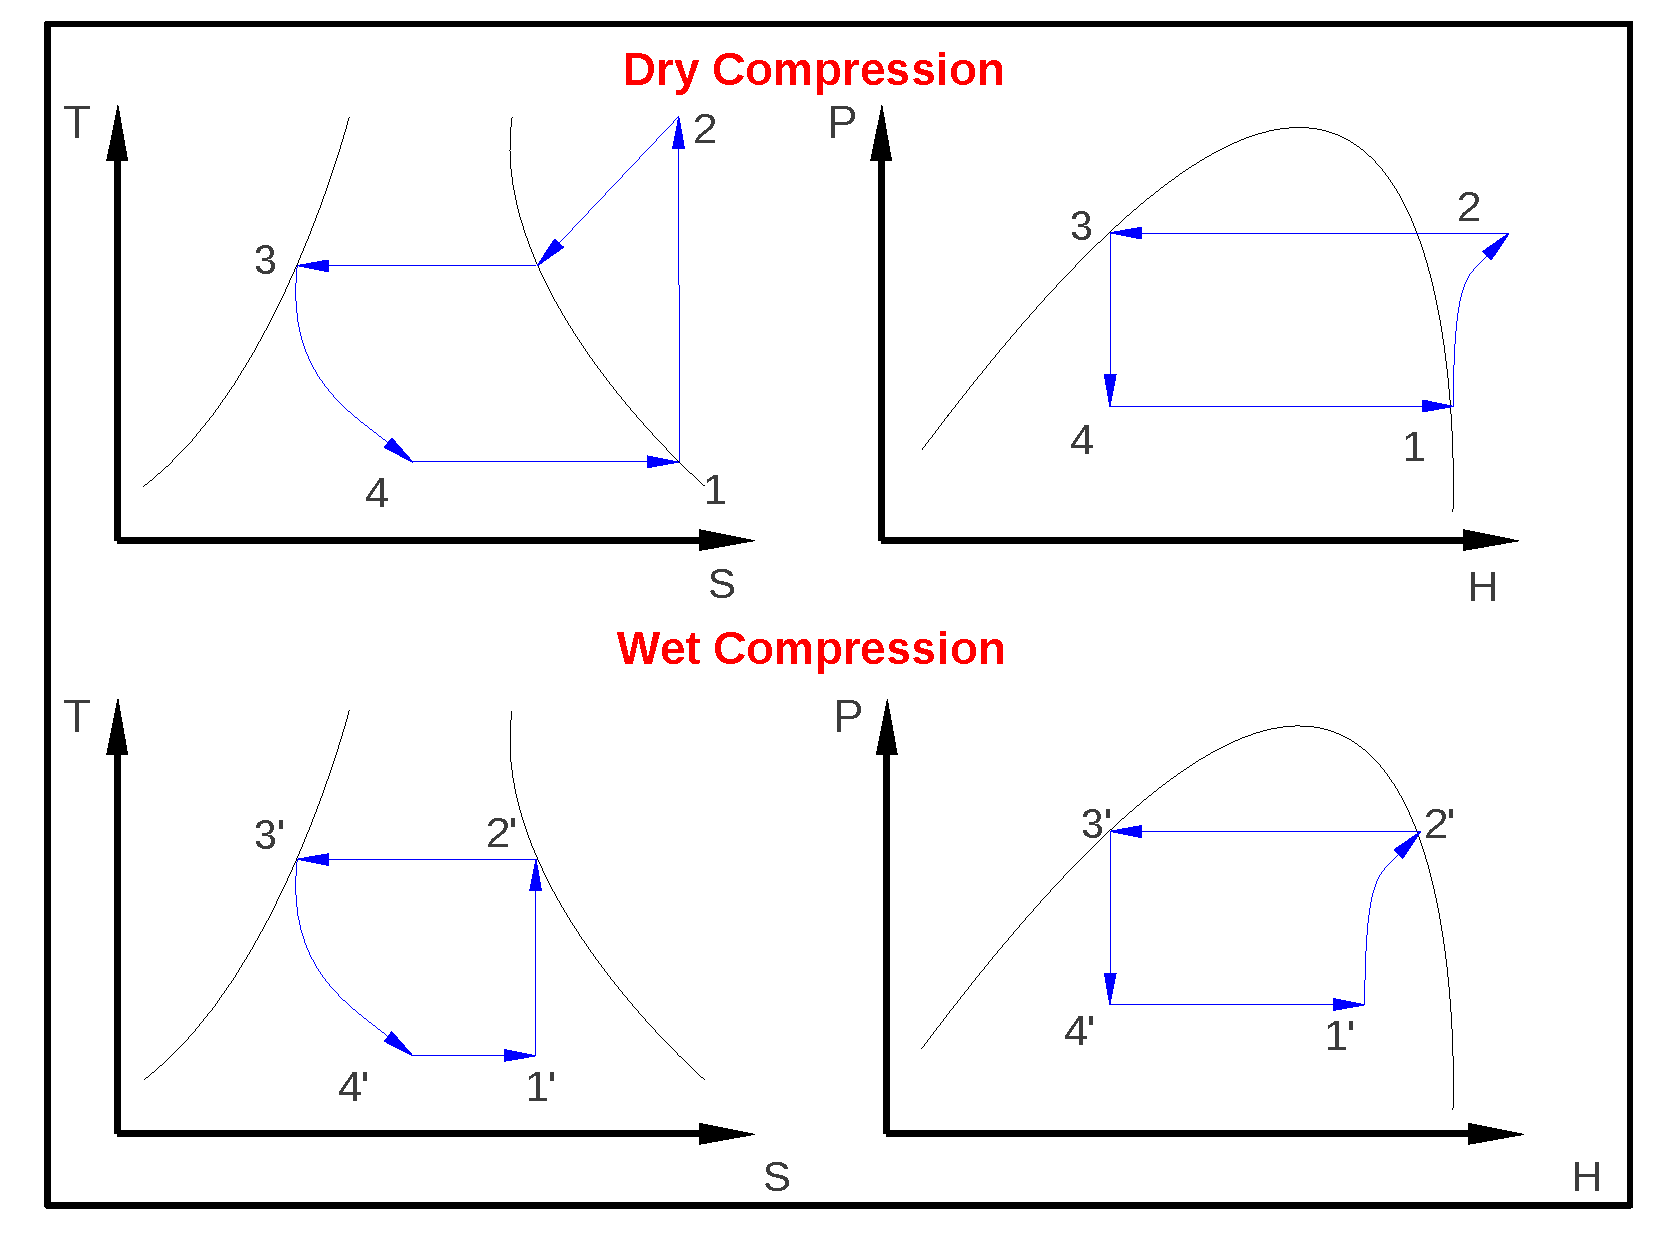
\includegraphics[width=4.5cm,clip]{./Pics/Overview_Refrig13}}
    \end{figure}  
   \end{column}  
   \begin{column}[c]{0.45\linewidth}
  \begin{enumerate}[(a)]
   \item <1-> In most industrial applications, vapour compression systems occur in closed cycles;
   \item <2-> Refrigerant (in gas/vapour phase) is compressed isentropically in \textcolor{blue}{compressor from state 1 to 2}; 
   \item <3-> \textcolor{blue}{High pressure and high temperature} fluid enters the condenser at \textcolor{blue}{state 2};
   \item <4-> The condensed fluid (saturated liquid at high pressure, state 3) is driven into the expansion valve where an \textcolor{blue}{isenthalpic expansion} occurs.
  \end{enumerate}
 \end{column}  
\end{columns}
\end{frame}


%%%
%%% Slide
%%%
\begin{frame}
 \frametitle{Description of the Cycle -- Dry Compression}
  \begin{columns}
   \begin{column}[c]{0.5\linewidth}
    \begin{figure}%
     \vbox{
      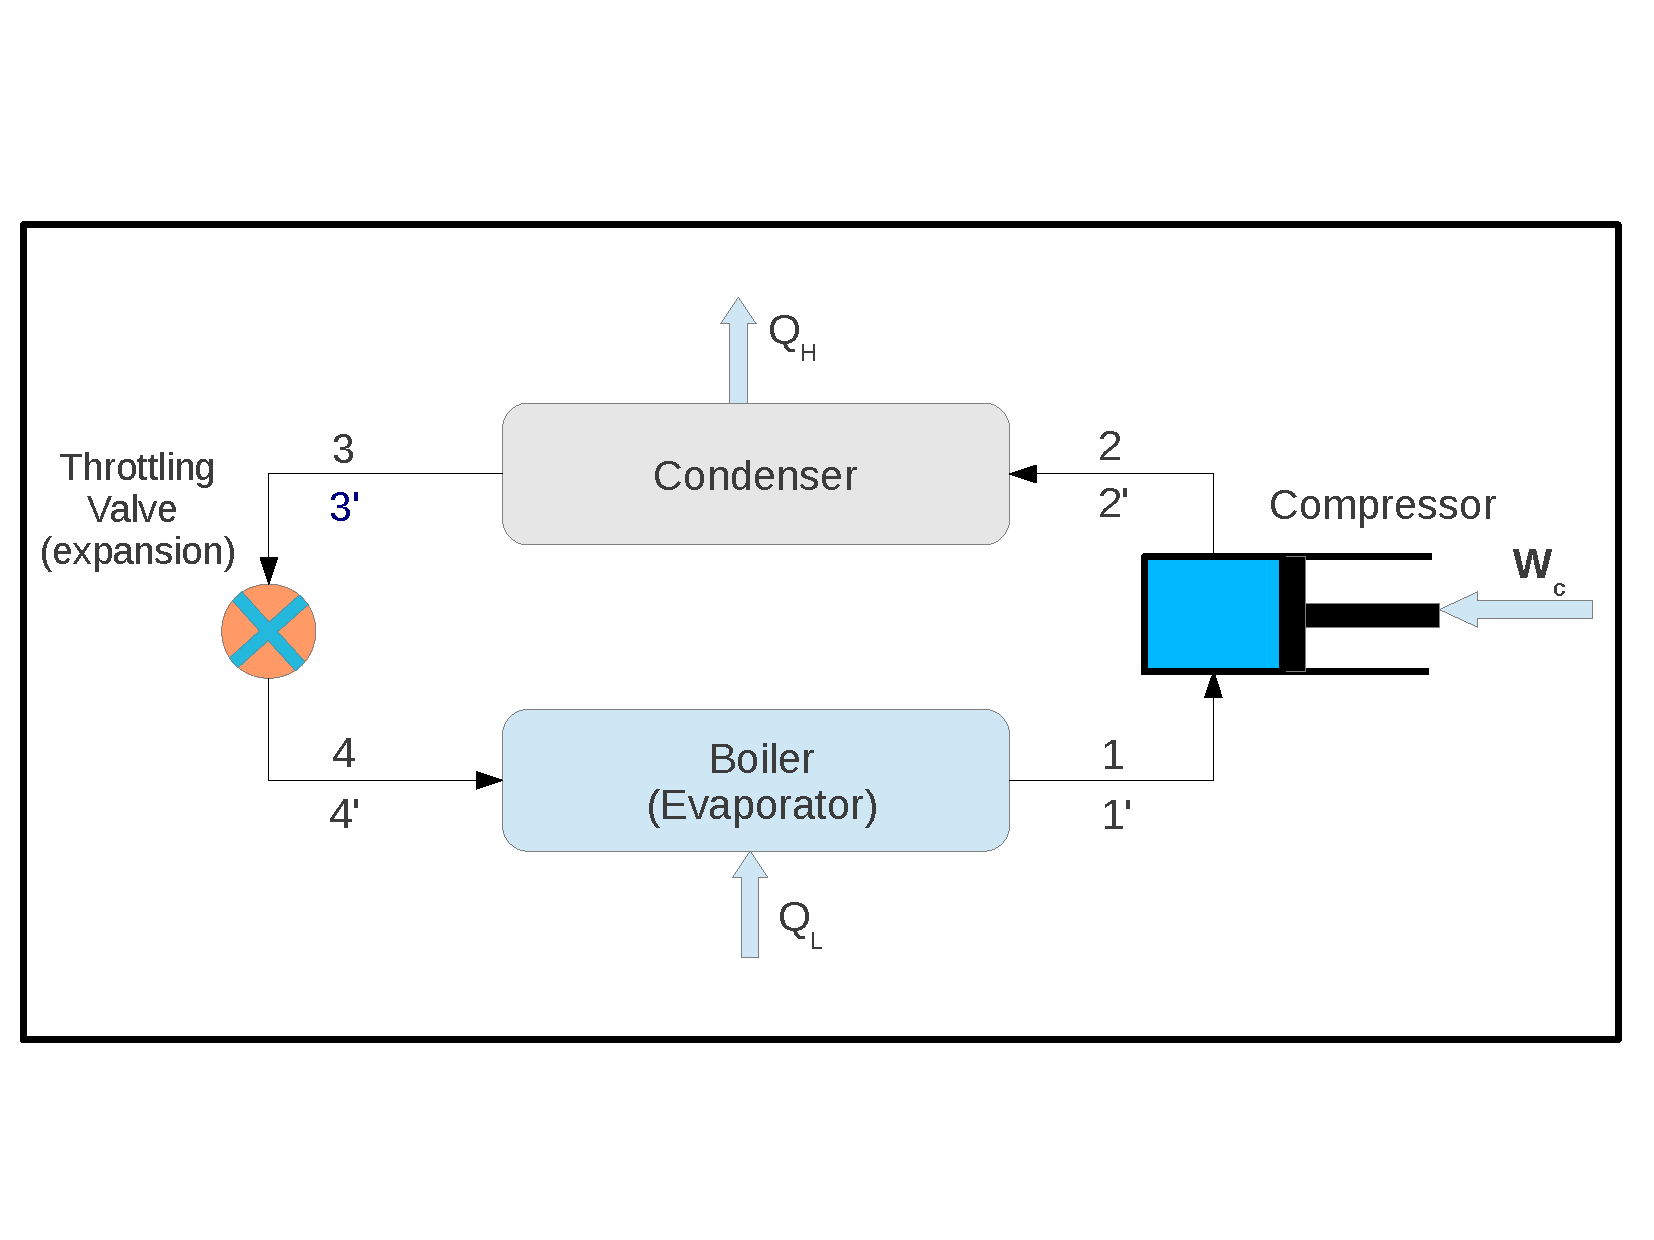
\includegraphics[width=5.5cm,clip]{./Pics/Overview_Refrig12}
      \vspace{-.5cm}
      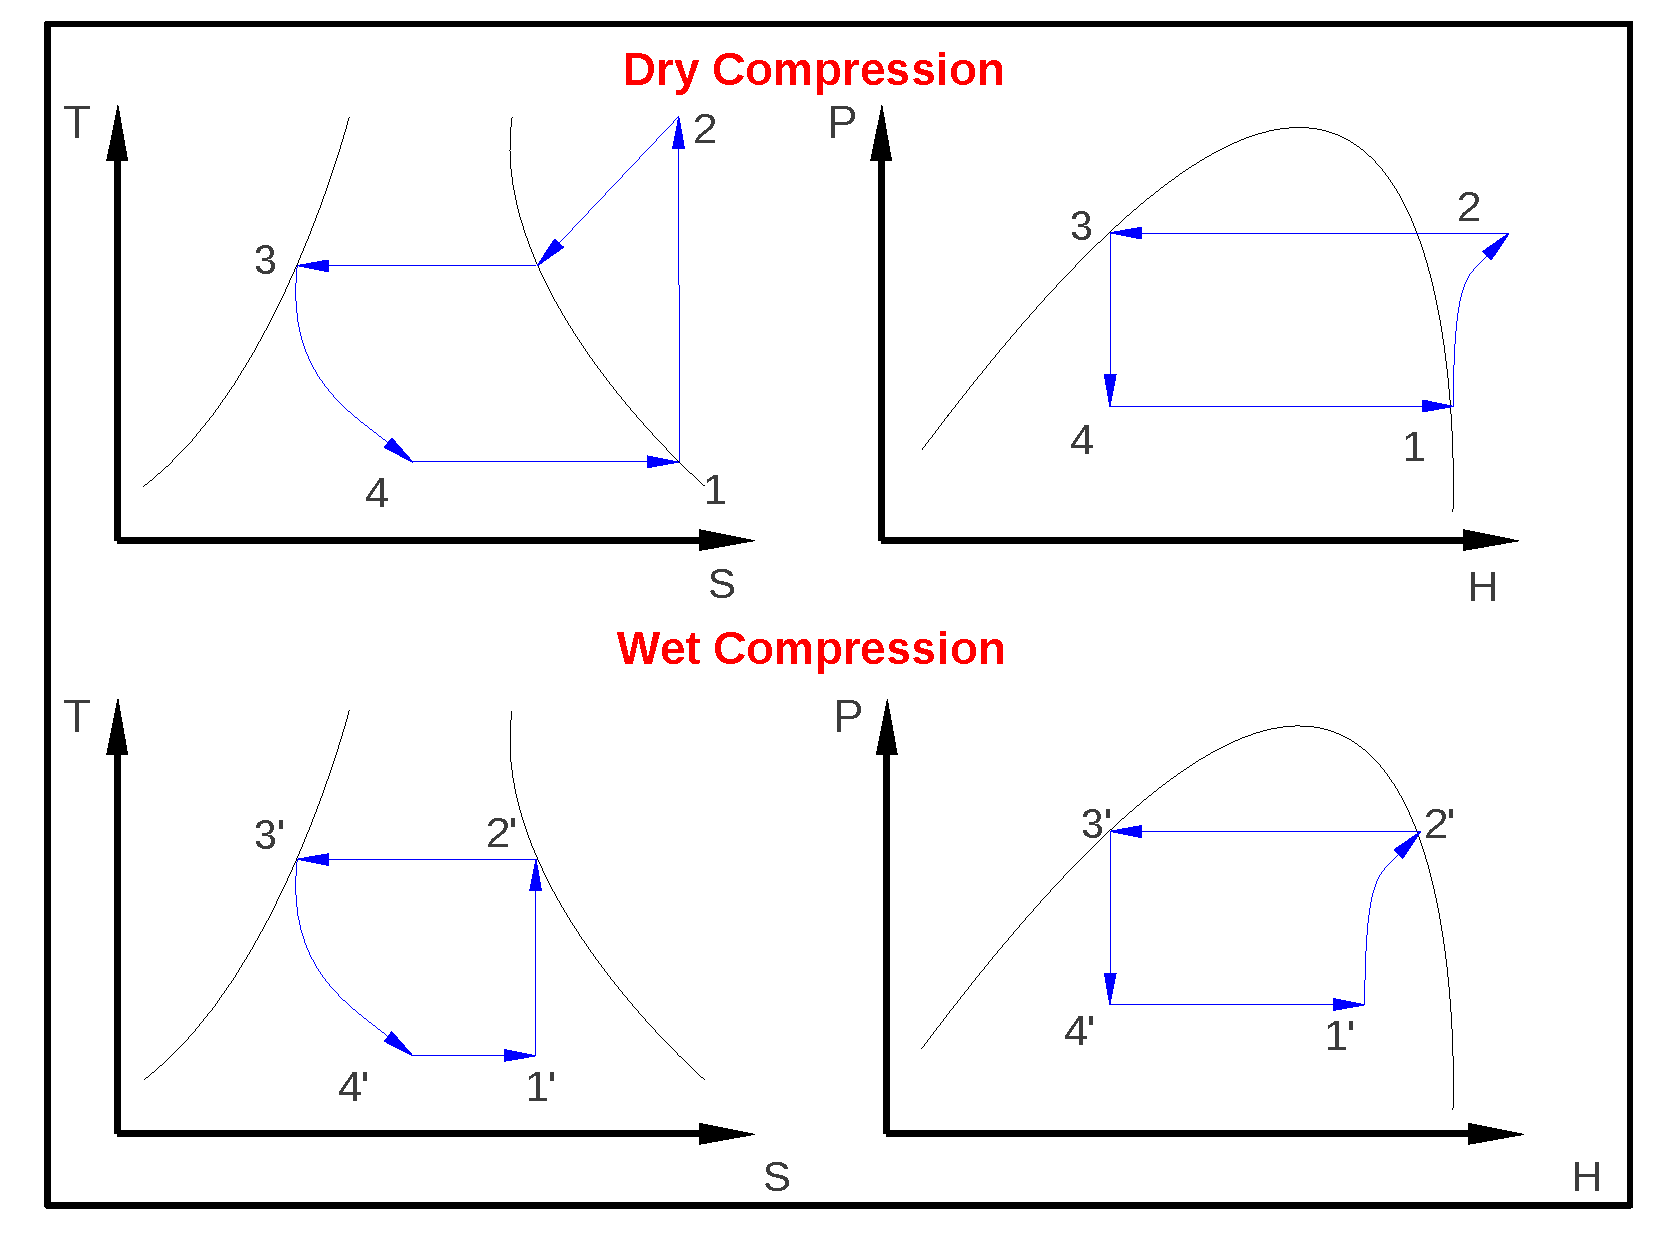
\includegraphics[width=4.5cm,clip]{./Pics/Overview_Refrig13}}
    \end{figure}  
   \end{column}  
   \begin{column}[c]{0.5\linewidth}
  \begin{enumerate}[(a)]
   \item <1-> The refrigerant fluid leaves the expansion valve (state 4) as a \textcolor{blue}{low pressure wet mixture of liquid and vapour};
   \item <2-> This mixture is driven into the evaporator where heat is transferred from the surroundings and thereby showing refrigerant effect; 
   \item <3-> Due to this \textcolor{blue}{heat absorption}, the liquid-vapour mixture is transformed into a \textcolor{red}{dry gaseous refrigerant} and;
   \item <4-> This process is called \textcolor{blue}{Dry Compression} in which,
   \item <5-> The compression of this dry refrigerant yields \textcolor{blue}{superheated state} of the fluid as shown in \textcolor{blue}{state 2}.
  \end{enumerate}
 \end{column}  
\end{columns}
\end{frame}


%%%
%%% Slide
%%%
\begin{frame}
 \frametitle{Description of the Cycle -- Wet Compression}
  \begin{columns}
   \begin{column}[c]{0.5\linewidth}
    \begin{figure}%
     \vbox{
      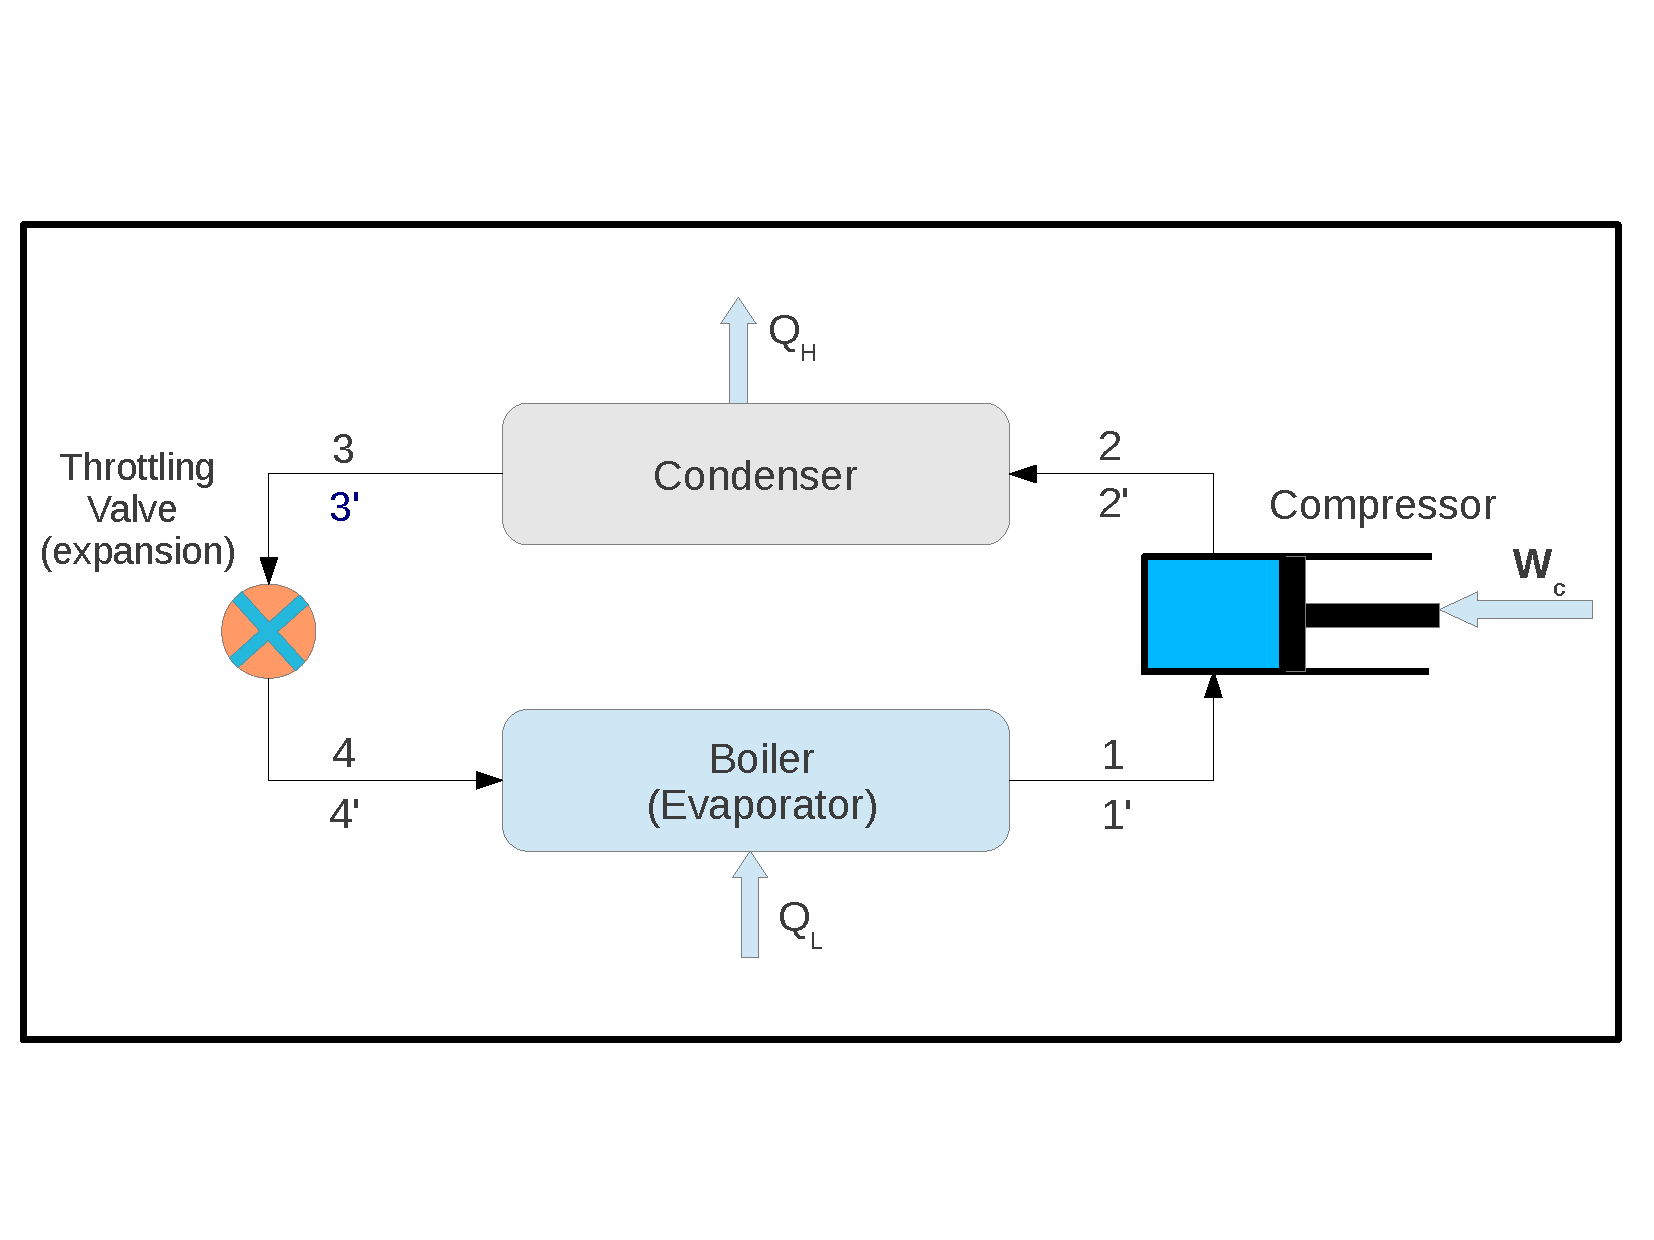
\includegraphics[width=5.5cm,clip]{./Pics/Overview_Refrig12}
      \vspace{-.5cm}
      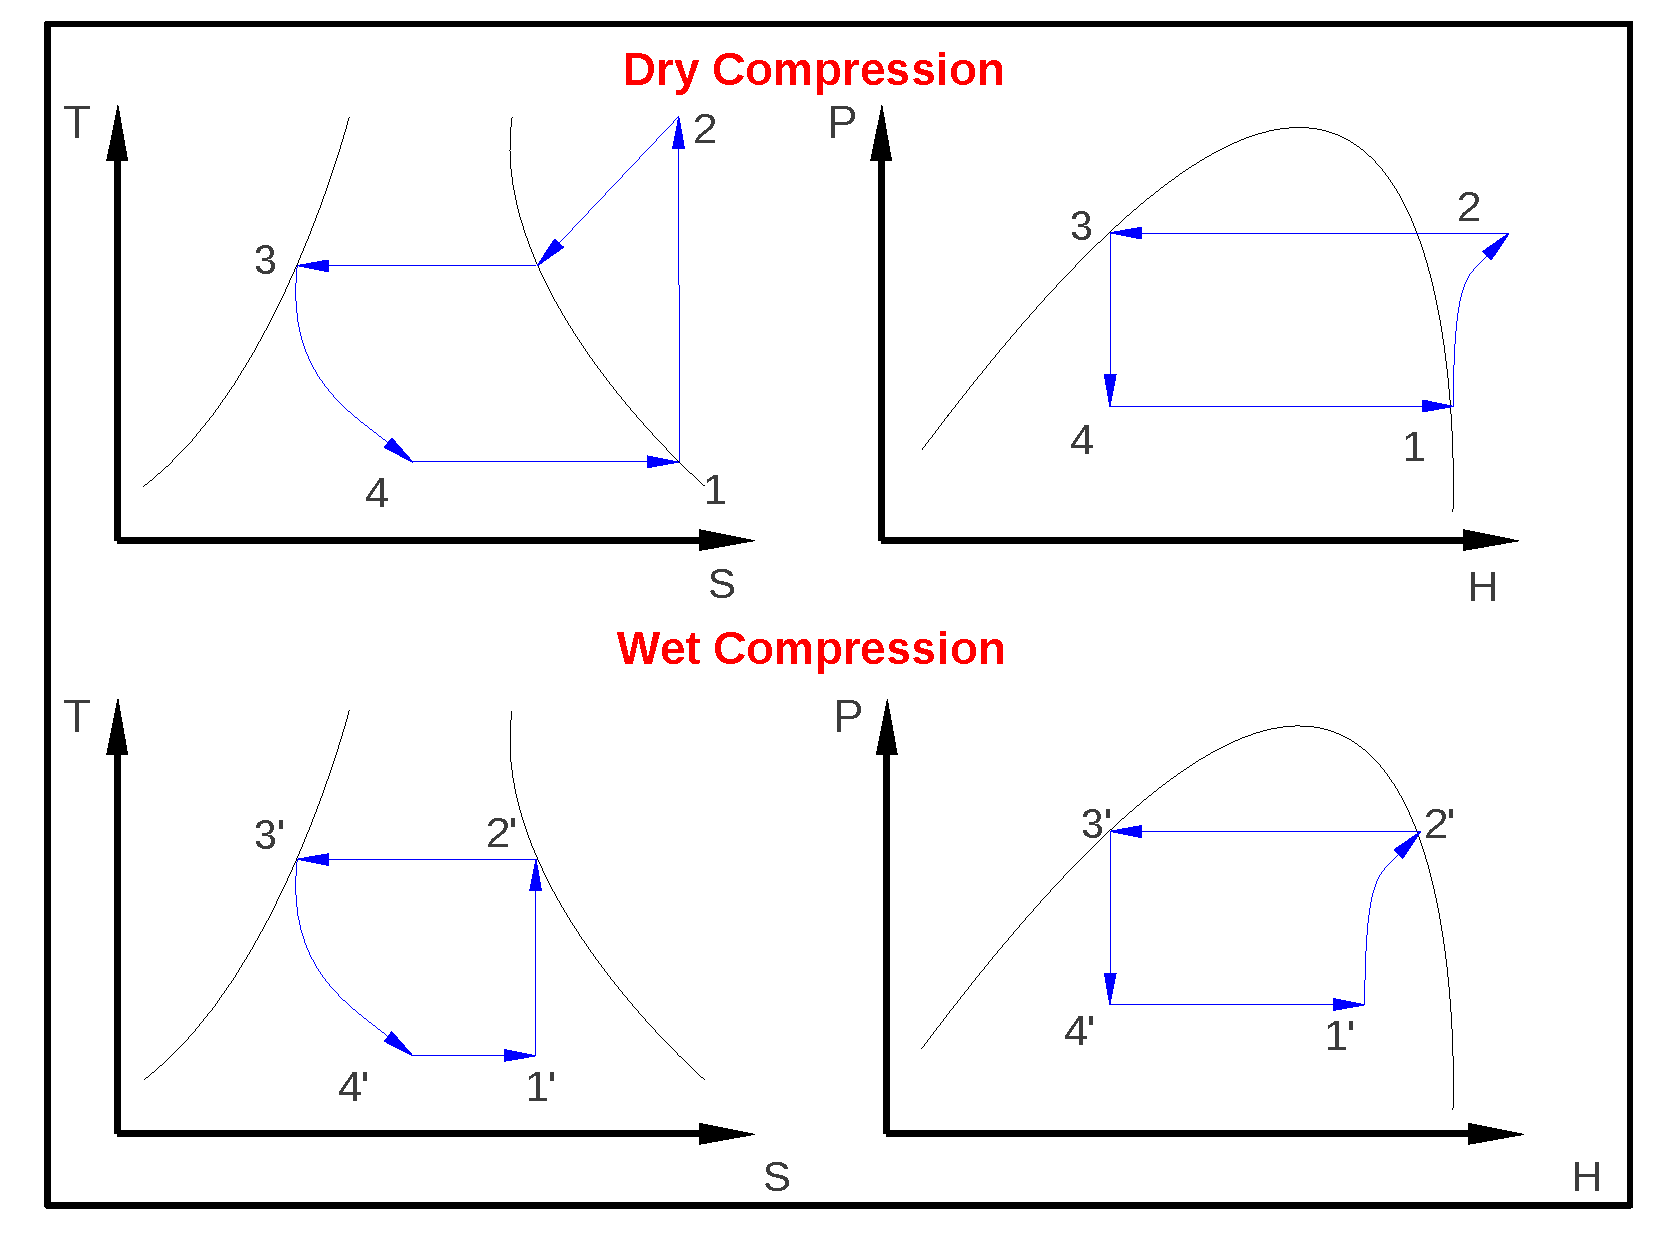
\includegraphics[width=4.5cm,clip]{./Pics/Overview_Refrig13}}
    \end{figure}  
   \end{column}  
   \begin{column}[c]{0.5\linewidth}
  \begin{enumerate}[(a)]
   \item <1-> In this case, the \textcolor{blue}{liquid-vapour mixture (state 1$^{\prime}$)} is injected in the compressor;
   \item <2-> In the compressor, the wet mixture is transformed into a \textcolor{blue}{dry refrigerant fluid} (gas phase -- state 2$^{\prime}$);
   \item <3-> The dry refrigerant at \textcolor{blue}{high pressure and high temperature} is driven into the condenser where the fluid is turned into saturated liquid at high pressure;
  \end{enumerate}
 \end{column}  
\end{columns}
\end{frame}



%%%
%%% Slide
%%%
\begin{frame}
 \frametitle{Description of the Cycle -- Wet Compression}
  \begin{columns}
   \begin{column}[c]{0.5\linewidth}
    \begin{figure}%
     \vbox{
      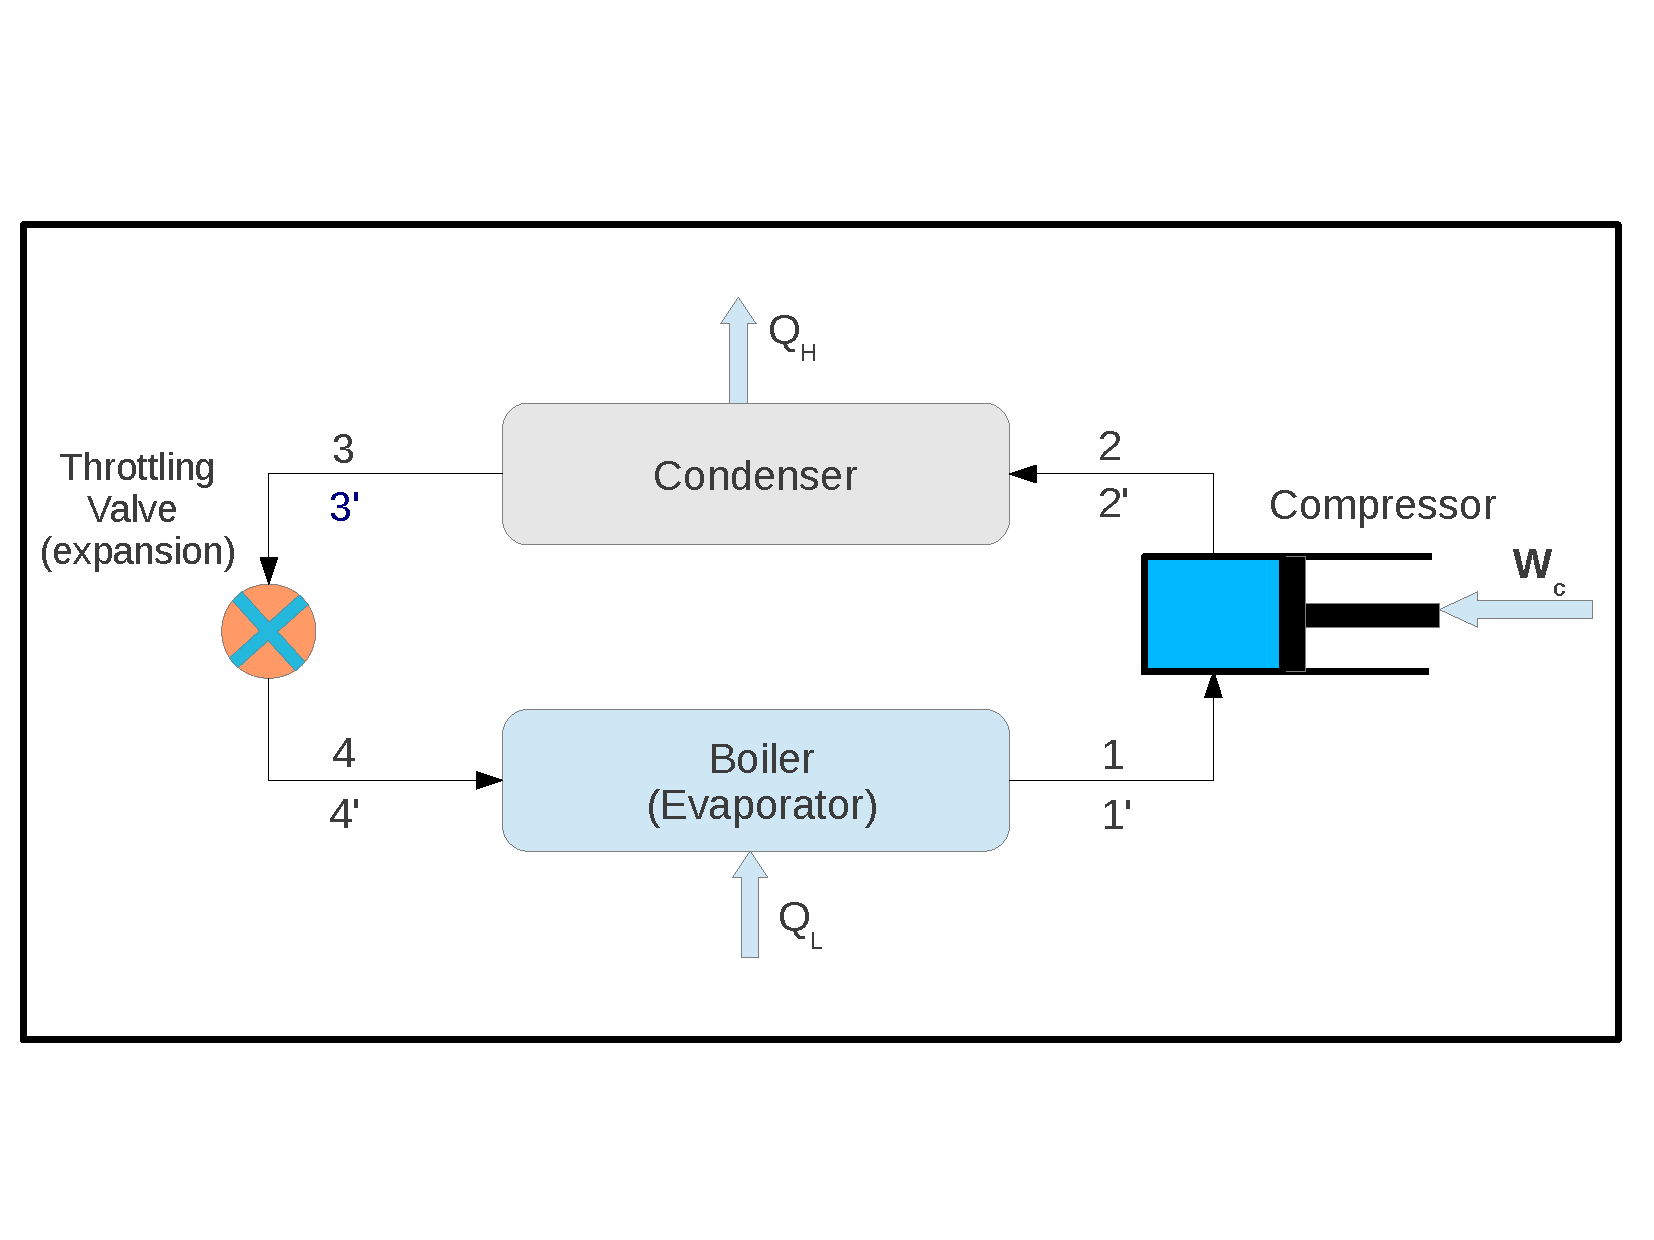
\includegraphics[width=5.5cm,clip]{./Pics/Overview_Refrig12}
      \vspace{-.5cm}
      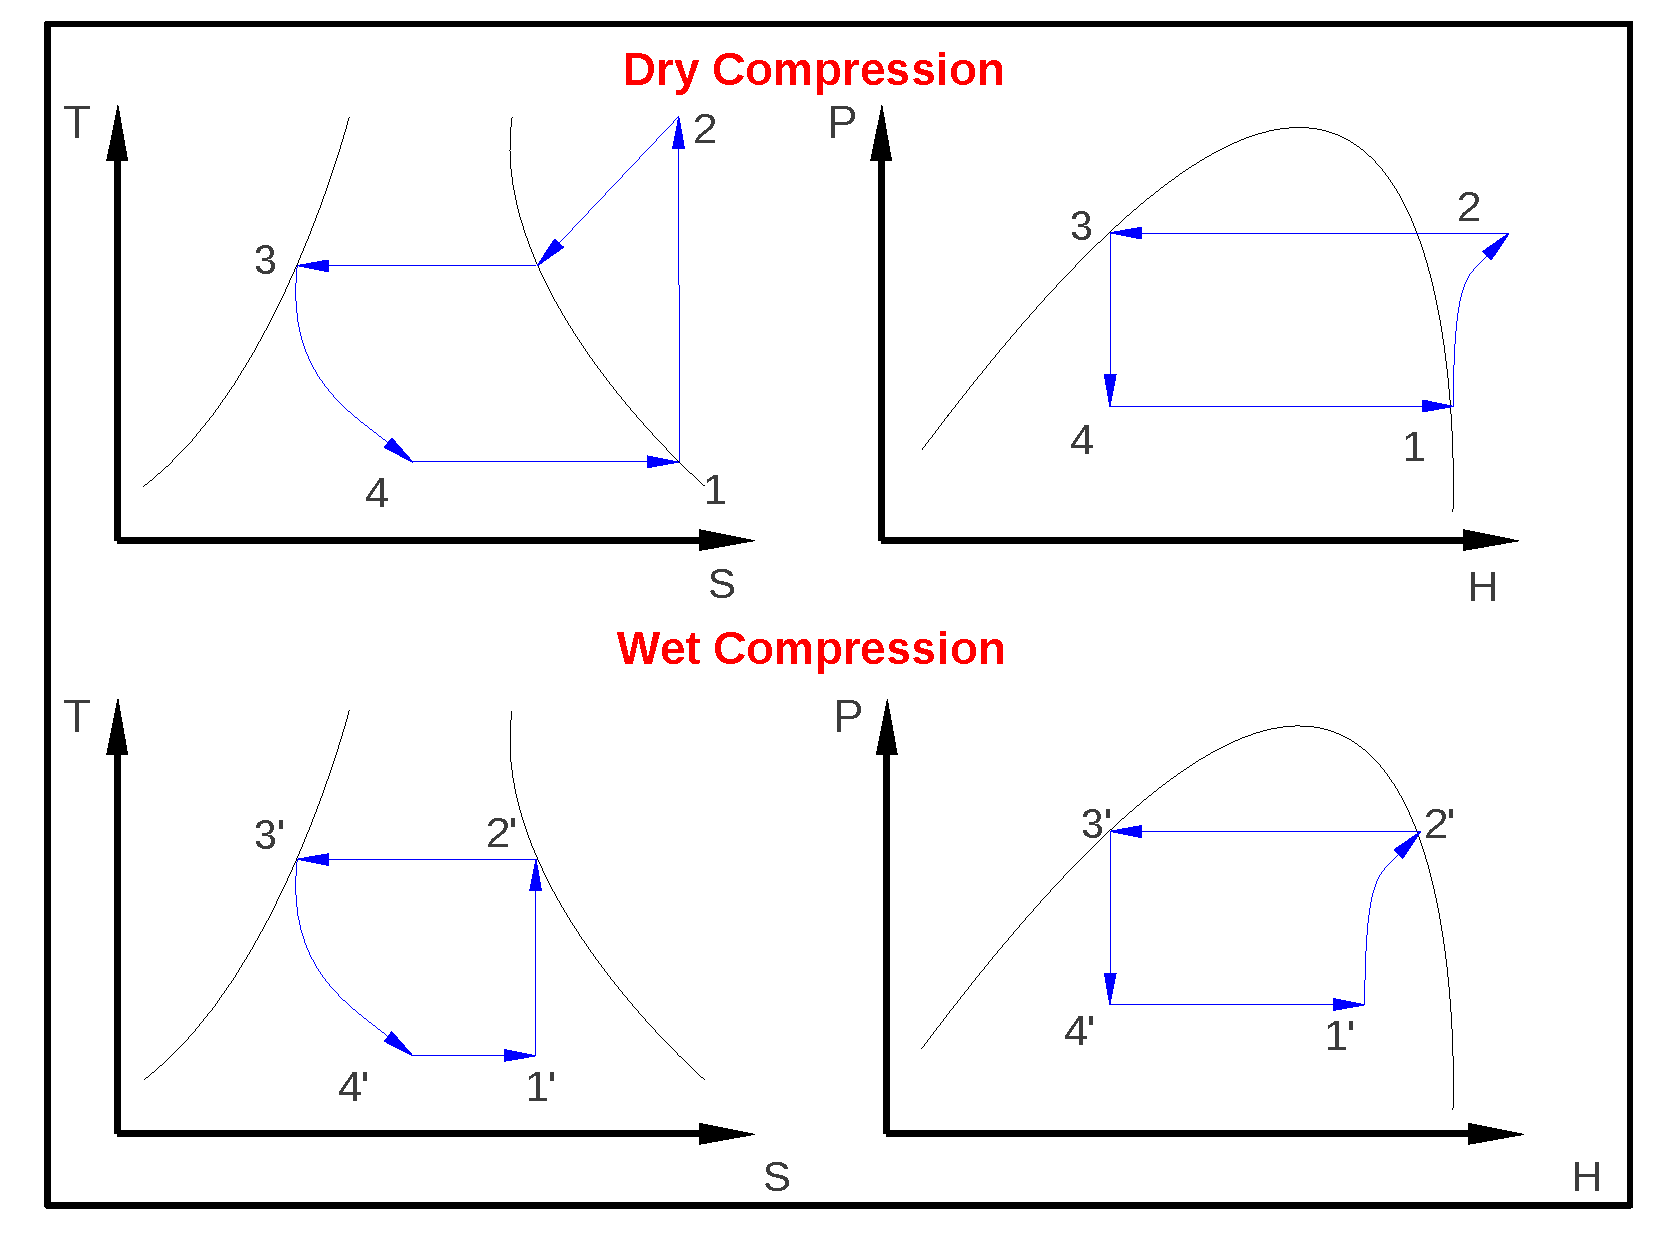
\includegraphics[width=4.5cm,clip]{./Pics/Overview_Refrig13}}
    \end{figure}  
   \end{column}  
   \begin{column}[c]{0.5\linewidth}
  \begin{enumerate}[(a)]
   \item <1-> The refrigerant is throttled from high to low pressure inside the expansion valve (states 3$^{\prime}$-4$^{\prime}$);
   \item <2-> The refrigerant is then driven towards the evaporator (states 4$^{\prime}$ 1$^{\prime}$) where it absorbs heat from the surroundings and ;
   \item <3-> Part of the liquid fraction is evaporated \textcolor{red}{but it does not become dry (gas) refrigerant} at the inlet of the compressor.
  \end{enumerate}
 \end{column}  
\end{columns}
\end{frame}



%%%
%%% Slide
%%%
\begin{frame}
 \frametitle{Description of the Cycle}
  \begin{columns}
   \begin{column}[c]{0.5\linewidth}
    \begin{figure}%
     \vbox{
      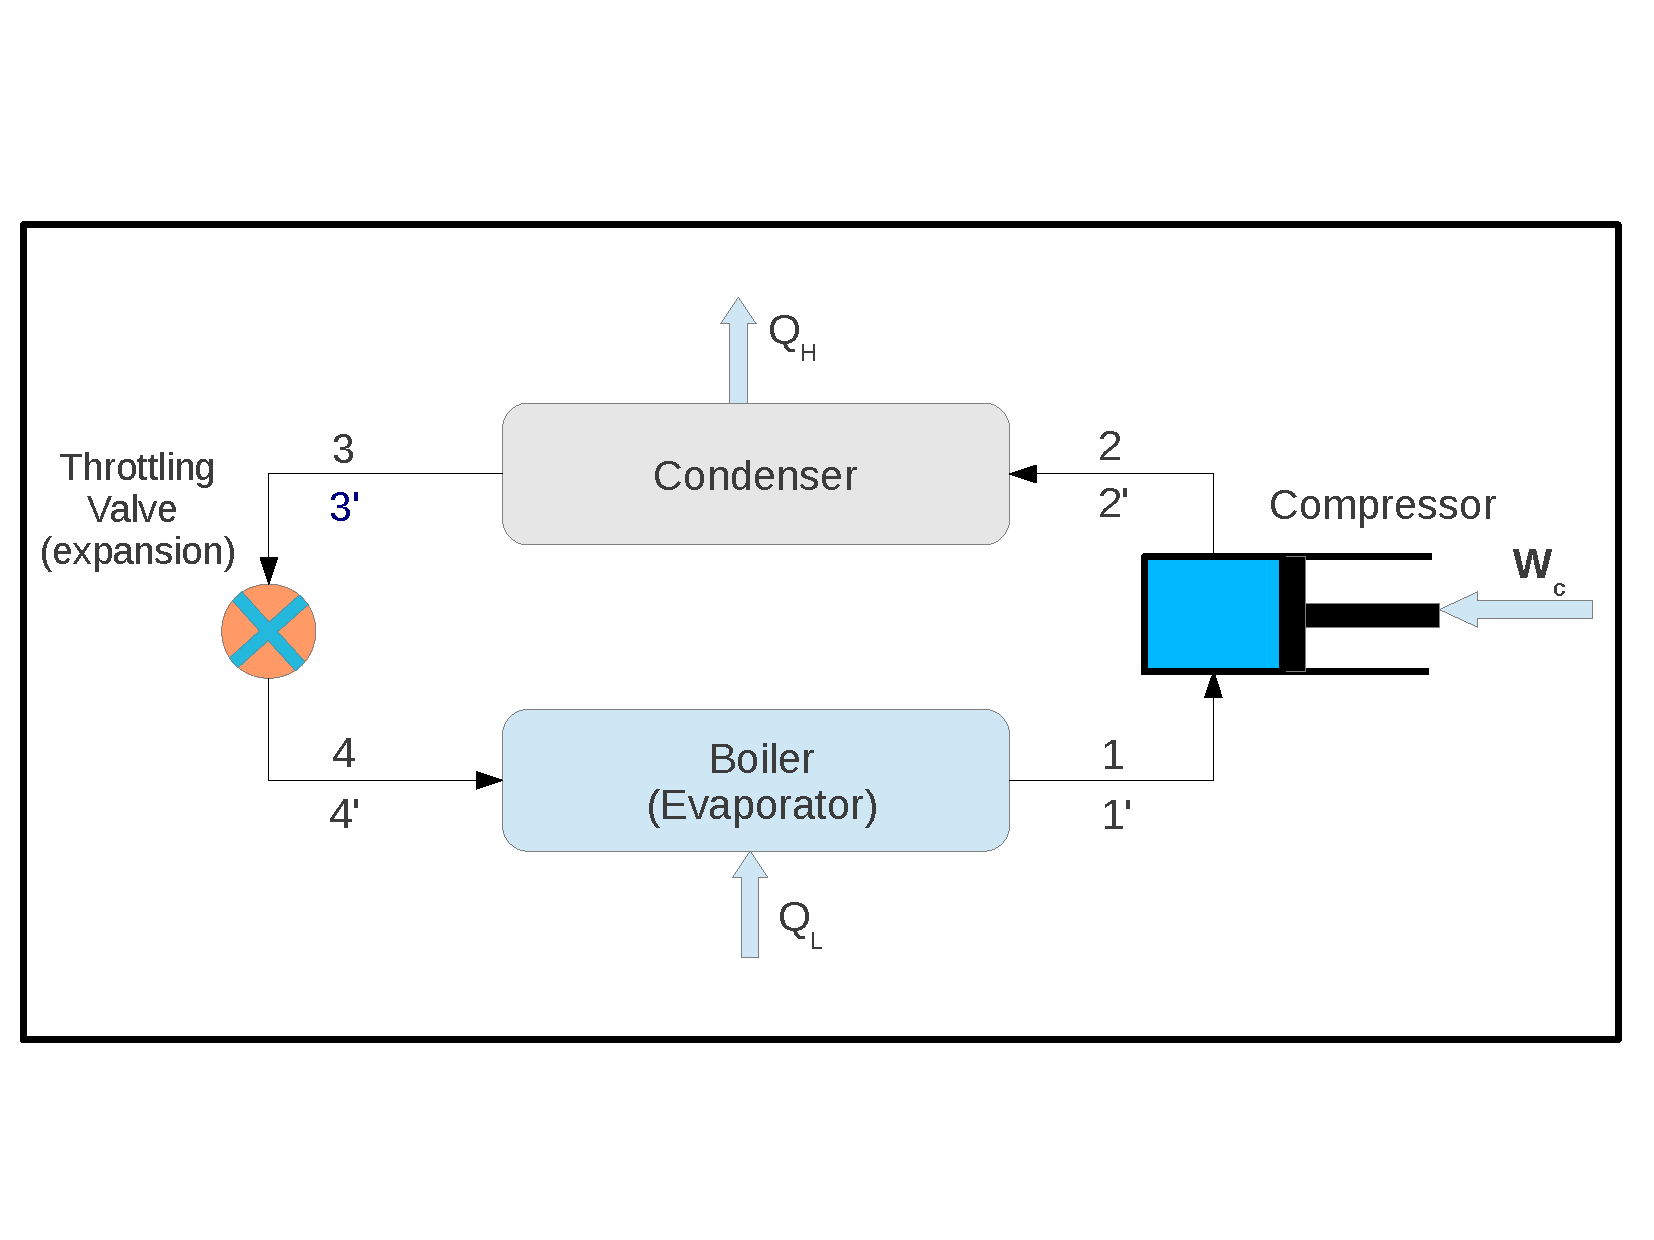
\includegraphics[width=5.5cm,clip]{./Pics/Overview_Refrig12}
      \vspace{-.5cm}
      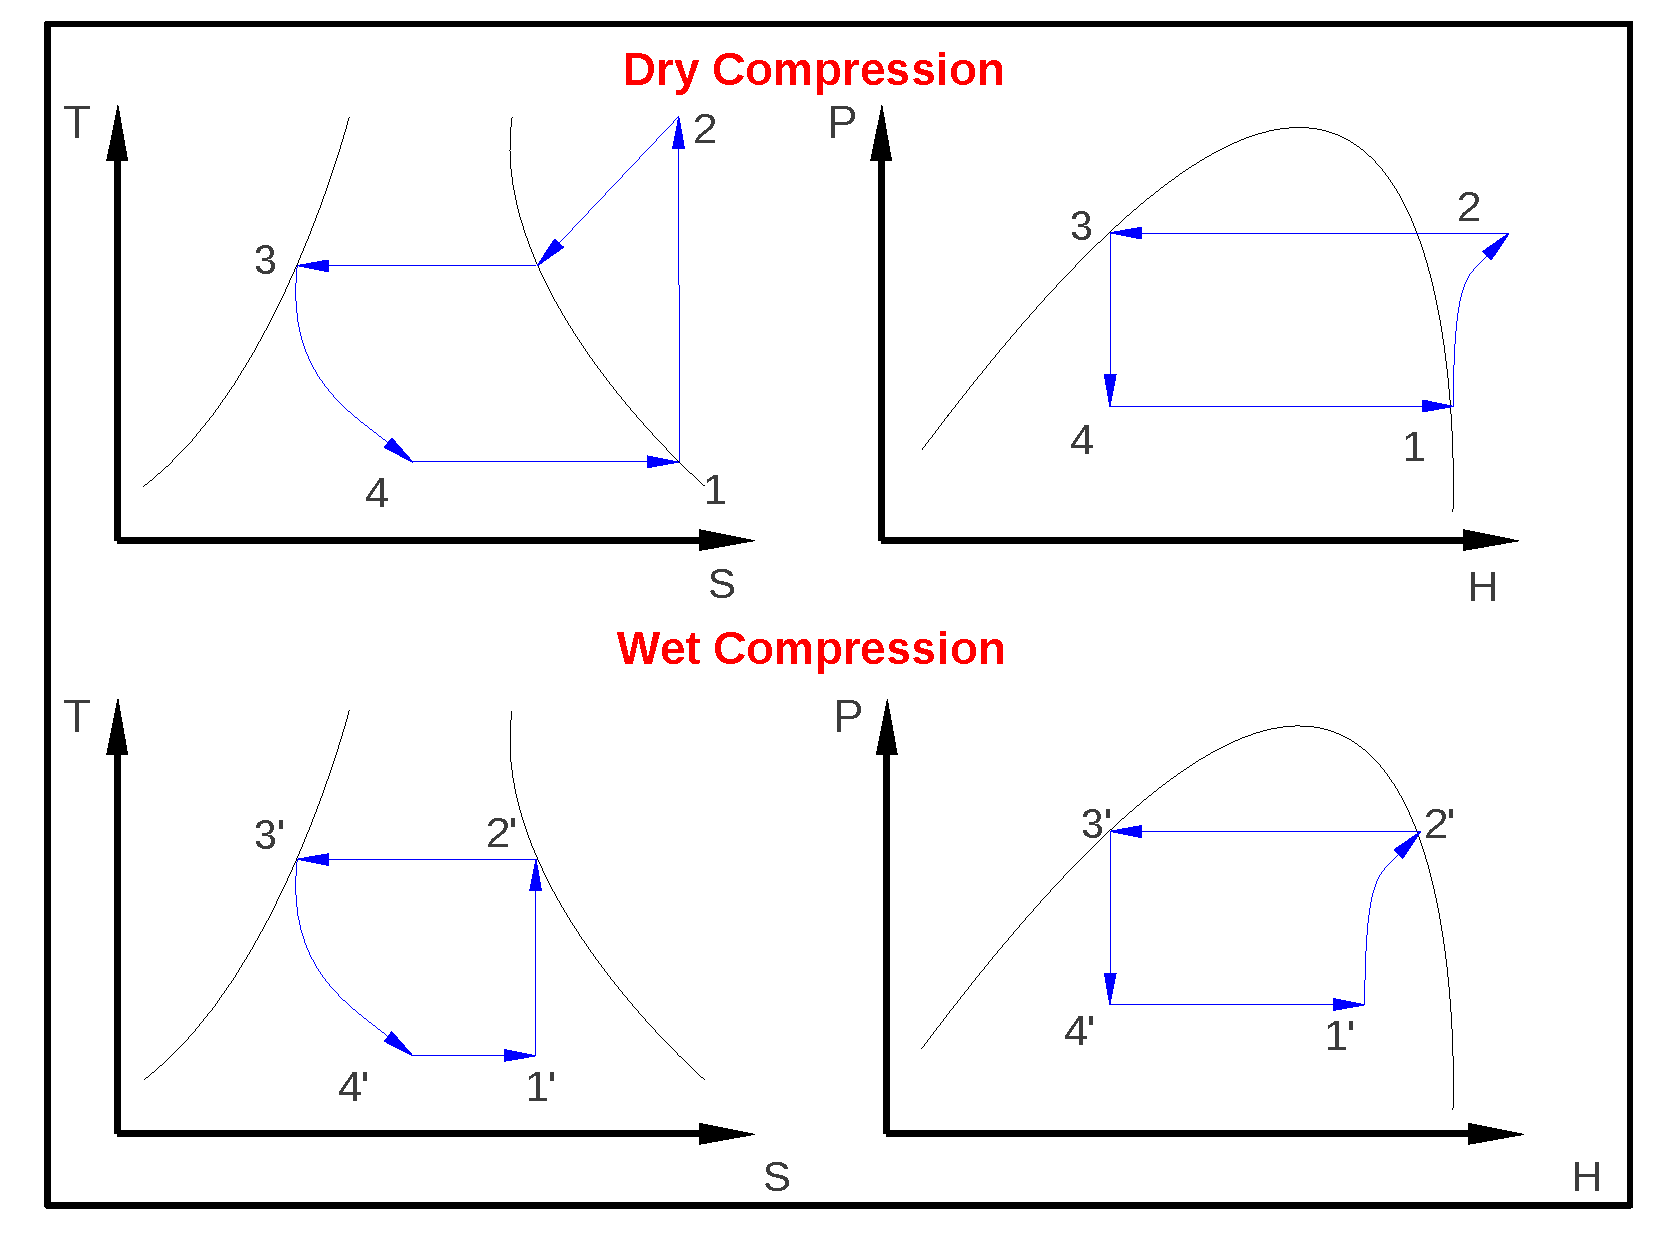
\includegraphics[width=4.5cm,clip]{./Pics/Overview_Refrig13}}
    \end{figure}  
   \end{column}  
   \begin{column}[c]{0.5\linewidth}
  \begin{itemize}
   \item <1-> \textcolor{blue}{1-2} or \textcolor{blue}{1$^{\prime}$-2$^{\prime}$:} isentropic compression;
   \item <1-> \textcolor{blue}{2-3} or \textcolor{blue}{2$^{\prime}$-3$^{\prime}$:} isobaric heat rejection;
   \item <1-> \textcolor{blue}{3-4} or \textcolor{blue}{3$^{\prime}$-4$^{\prime}$:} isenthalpic expansion ;%process or throttling process;
   \item <1-> \textcolor{blue}{4-1} or \textcolor{blue}{4$^{\prime}$-1$^{\prime}$:} isobaric heat absorption.
  \end{itemize}
 \end{column}  
\end{columns}
\end{frame}


%%%
%%% Slide
%%%
\begin{frame}
 \frametitle{A few Notes}
\begin{enumerate}
\item <1-> The \textcolor{blue}{compressor efficiency} is often \textcolor{blue}{higher in dry-compression processes than in wet-compression} processes due to;
\item <2-> \textcolor{blue}{Larger volumetric efficiency} with dry refrigerant and also;
\item <3-> Smaller possibility of equipment damage using dry fluids;
\item <4-> During dry-compression the temperature of compressed refrigerant becomes larger than the condensation temperature;
\item <5-> Such large temperature after the compression leads to the necessity for cooling of the compressor;
\item <6-> Which can be done (and usually is) by using the same cooling flow used for cooling the condenser;
\item <7-> \textcolor{blue}{Cooling the compressor reduces the compression work}.
\end{enumerate}
\end{frame}



%%%
%%% Slide
%%%
\begin{frame}
 \frametitle{Thermal Analysis}
 \begin{columns}
  \begin{column}[c]{0.35\linewidth}
   \begin{figure}%
     \vbox{
      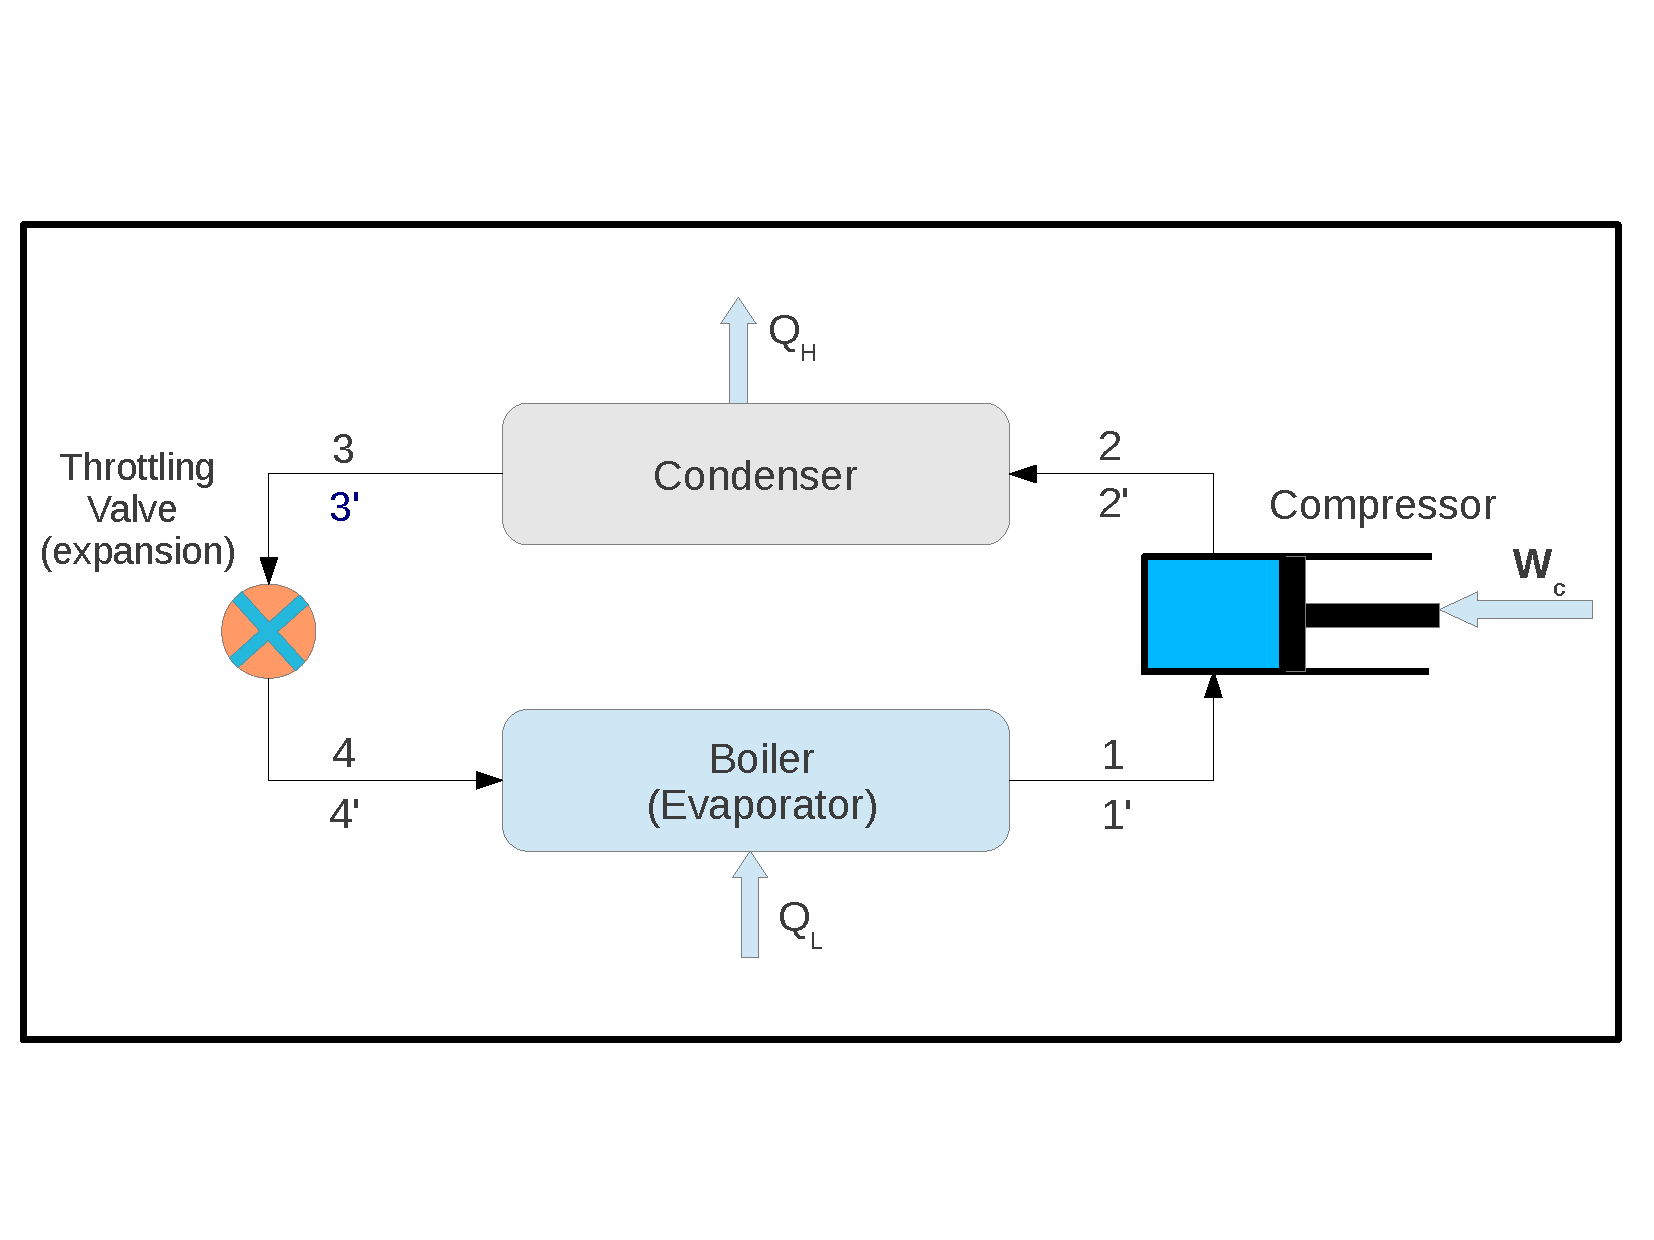
\includegraphics[width=4.5cm,clip]{./Pics/Overview_Refrig12}
      \vspace{-.5cm}
    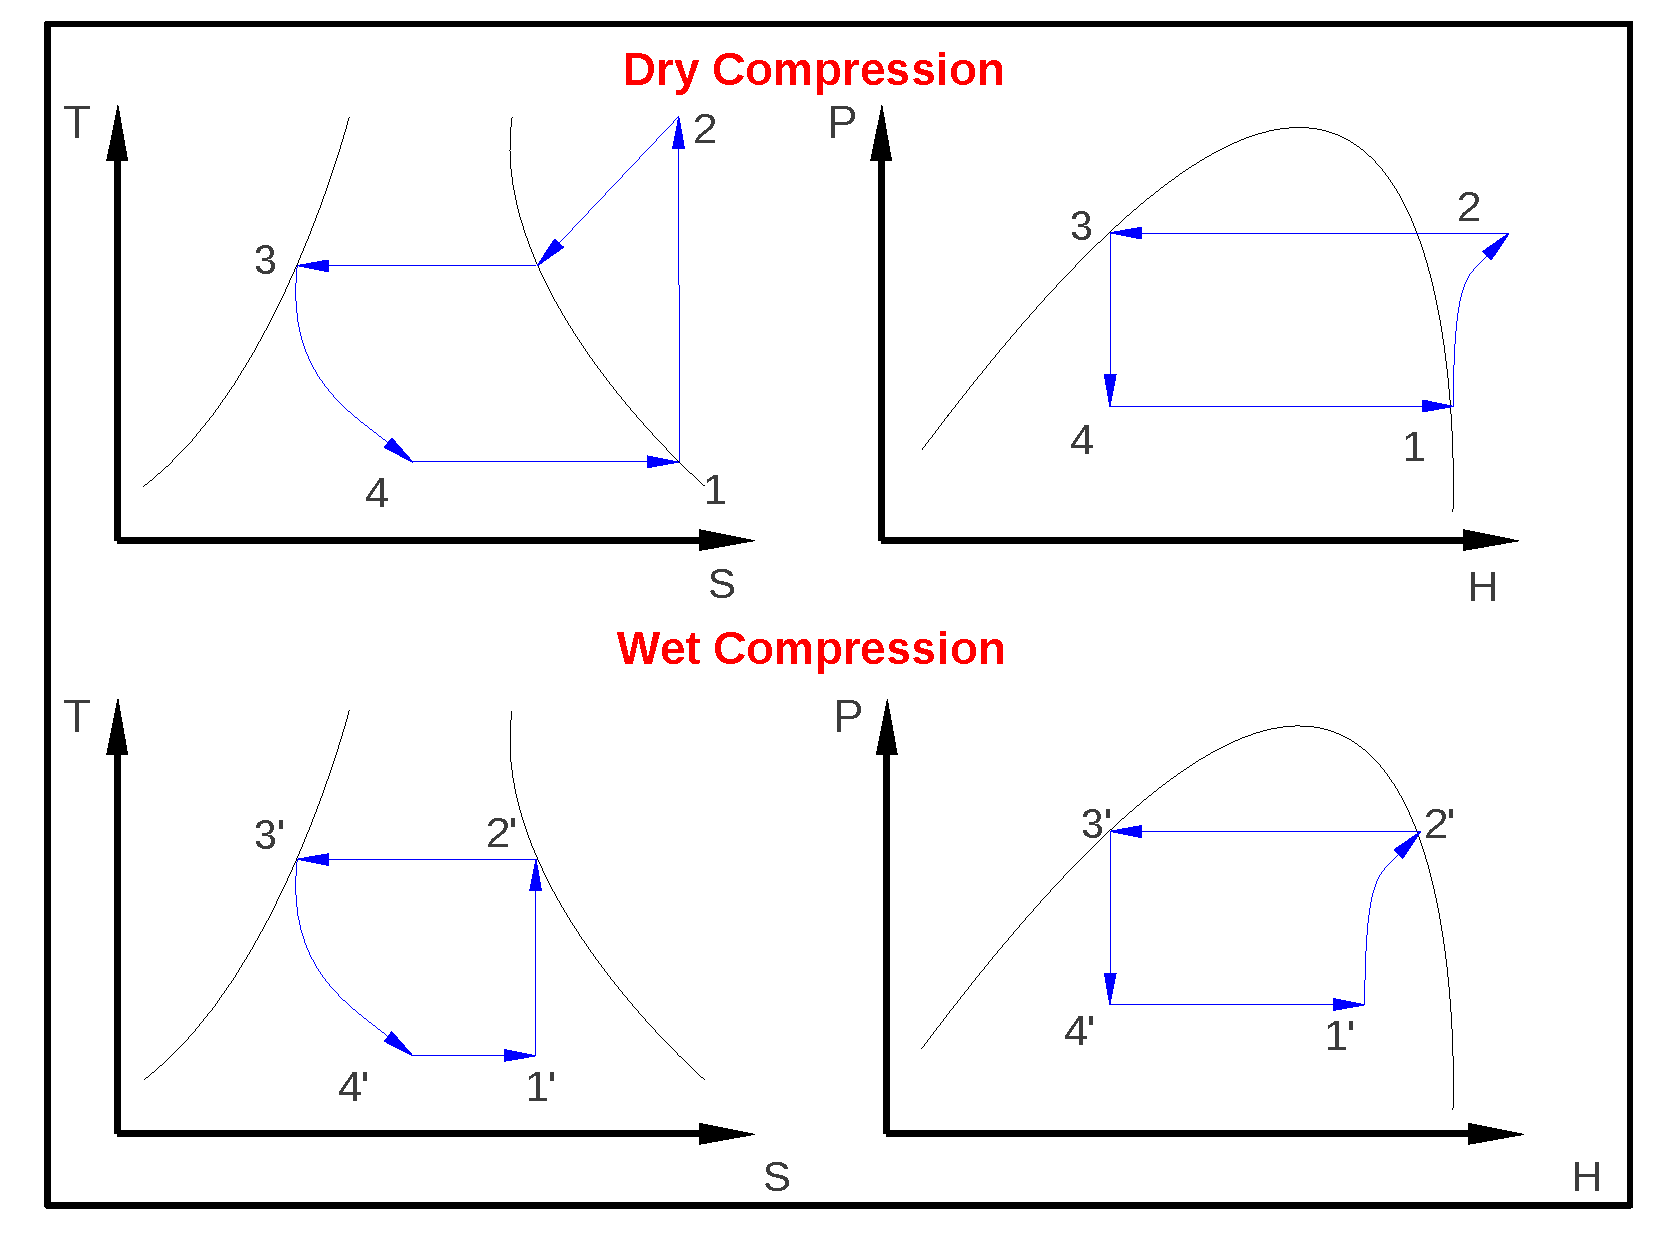
\includegraphics[width=4.5cm,clip]{./Pics/Overview_Refrig13}}
   \end{figure}  
  \end{column}  
  \begin{column}[c]{0.65\linewidth}
   \begin{enumerate}
    \item <1-> Let's assume that the mass flow rate of refrigerant is \textcolor{blue}{$\dot{m}$ (kg/s)};
    \item <2-> The \textcolor{blue}{refrigeration capacity} (or refrigeration effect) is,
       \begin{eqnarray}
        &&Q_{\text{absorbed}}^{\text{(dry)}} = \dot{m}\left(H_{1}-H_{4}\right) \nonumber \\
        &&Q_{\text{absorbed}}^{\text{(wet)}} = \dot{m}\left(H_{1^{\prime}}-H_{4^{\prime}}\right) \nonumber        
       \end{eqnarray}
     \item <3-> And the \textcolor{blue}{net work} (= work input) is,
       \begin{eqnarray}     
        &&W_{\text{compressor}}^{\text{(dry)}} = \dot{m}\left(H_{2}-H_{1}\right) \nonumber \\
        &&W_{\text{compressor}}^{\text{(wet)}} = \dot{m}\left(H_{2^{\prime}}-H_{1^{\prime}}\right) \nonumber
       \end{eqnarray}
   \end{enumerate}
  \end{column}  
 \end{columns}
\end{frame}



%%%
%%% Slide
%%%
\begin{frame}
 \frametitle{Thermal Analysis}
 \begin{columns}
  \begin{column}[c]{0.35\linewidth}
   \begin{figure}%
     \vbox{
      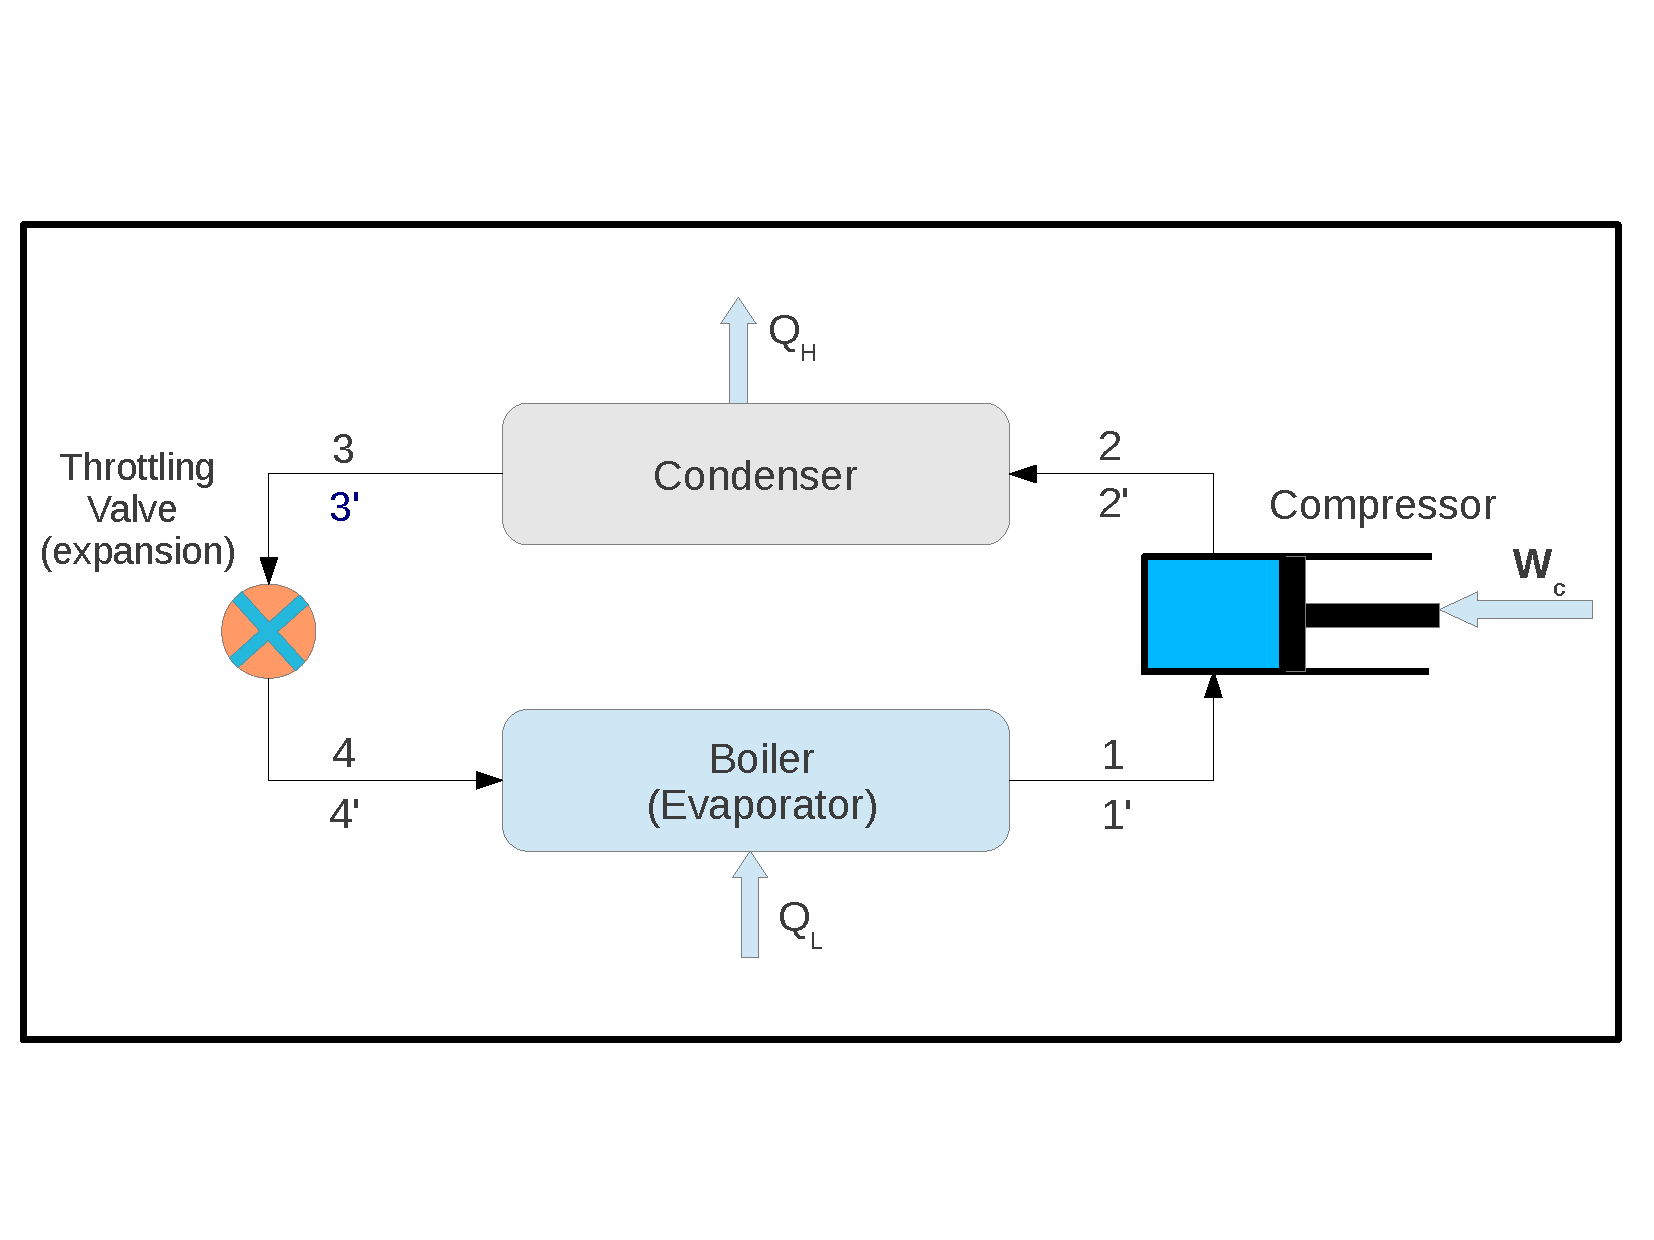
\includegraphics[width=4.5cm,clip]{./Pics/Overview_Refrig12}
      \vspace{-.5cm}
    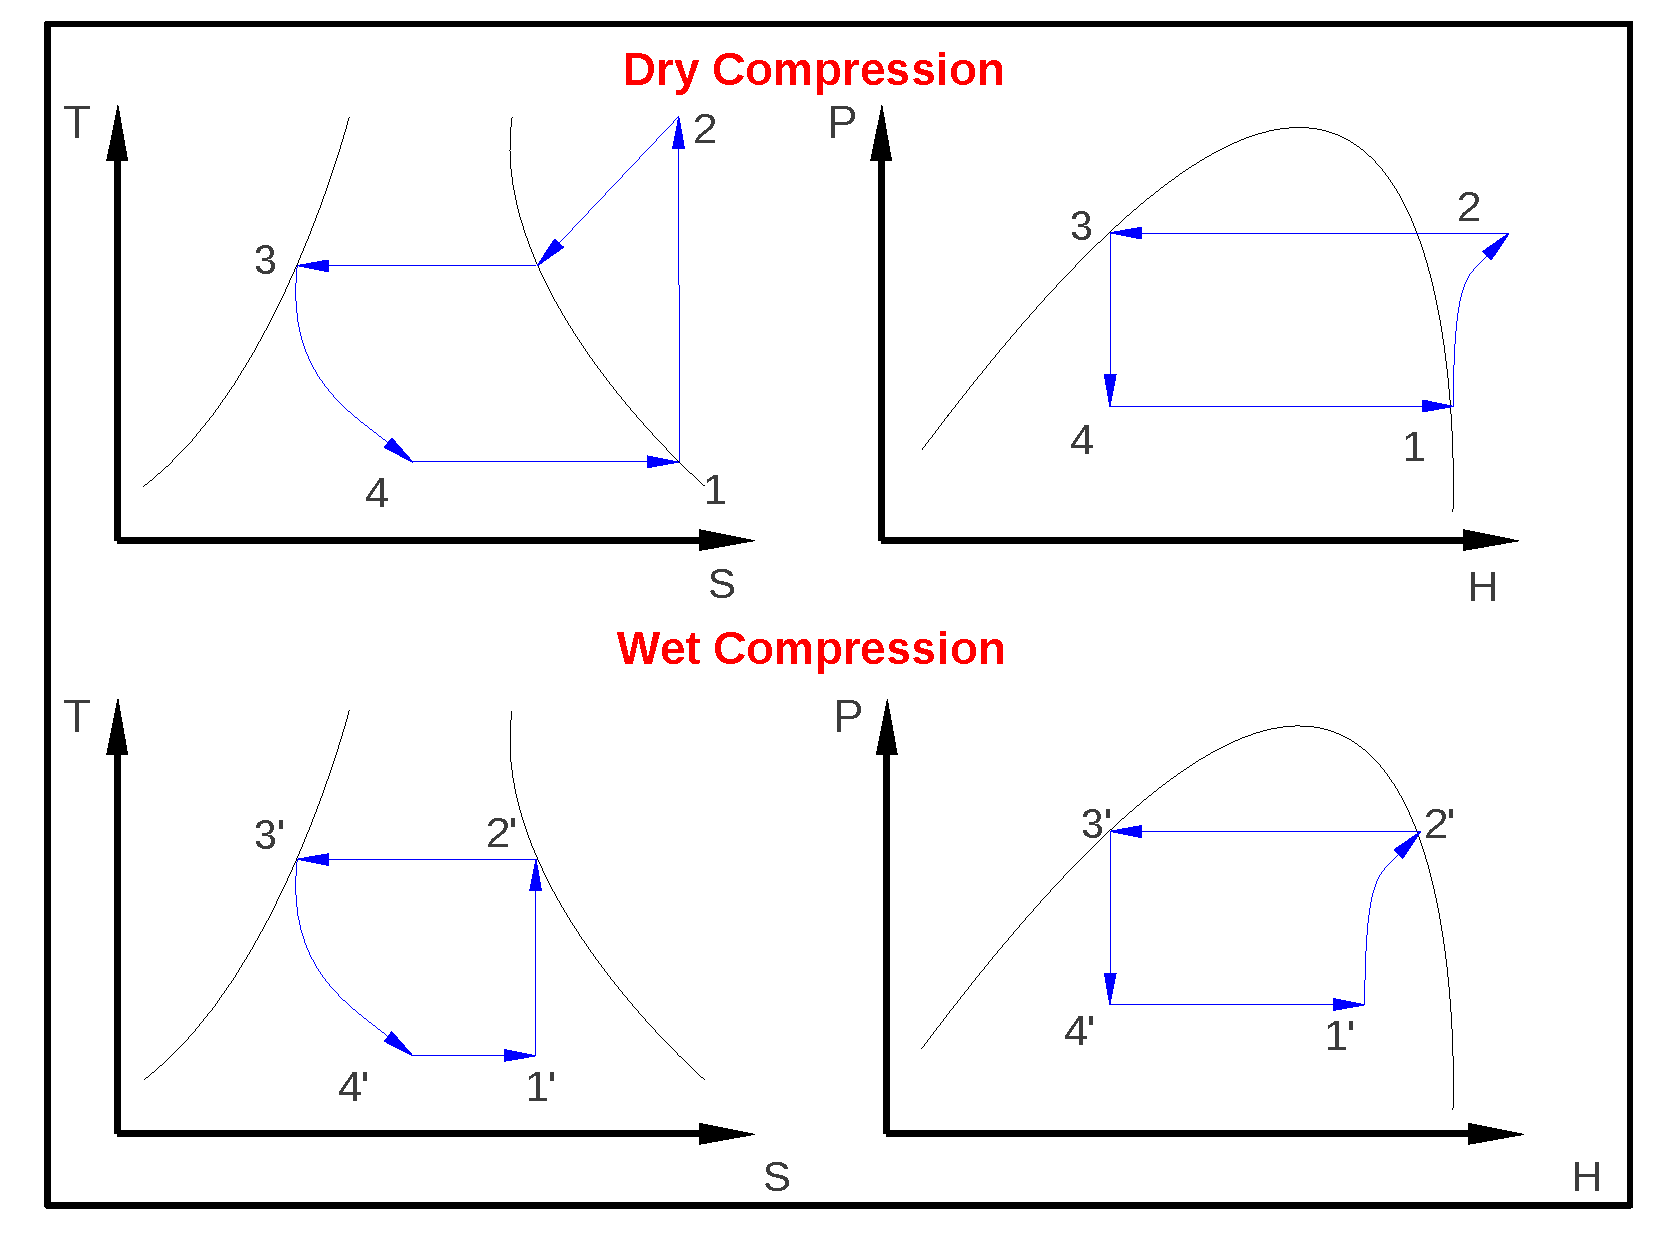
\includegraphics[width=4.5cm,clip]{./Pics/Overview_Refrig13}}
   \end{figure}  
  \end{column}  
  \begin{column}[c]{0.65\linewidth}
   \begin{itemize}
    \item <1-> And the \textcolor{blue}{Coefficient of Performance (COP)} is,
       \begin{eqnarray}
        \textcolor{blue}{COP^{\text{(dry)}}} &=& \textcolor{blue}{\frc{\text{Refrigeranting Capacity}}{\text{Work done}}} \nonumber \\
                       &=& \frc{\dot{m}\left(H_{1}-H_{4}\right)}{\dot{m}\left(H_{2}-H_{1}\right)} \nonumber \\
                       &=& \textcolor{blue}{\frc{H_{1}-H_{4}}{H_{2}-H_{1}}}       \nonumber
       \end{eqnarray}
     and
       \begin{eqnarray}
        \textcolor{blue}{COP^{\text{(wet)}}} &=& \frc{\dot{m}\left(H_{1^{\prime}}-H_{4^{\prime}}\right)}{\dot{m}\left(H_{2^{\prime}}-H_{1^{\prime}}\right)} \nonumber \\
                       &=& \textcolor{blue}{\frc{H_{1^{\prime}}-H_{4^{\prime}}}{H_{2^{\prime}}-H_{1^{\prime}}} }    \nonumber  
       \end{eqnarray}

   \end{itemize}
  \end{column}  
 \end{columns}
\end{frame}




%%%
%%% Slide
%%%
\begin{frame}
 \frametitle{Thermal Analysis}
 \begin{columns}
  \begin{column}[c]{0.65\linewidth}
   \begin{figure}%
     \vbox{
      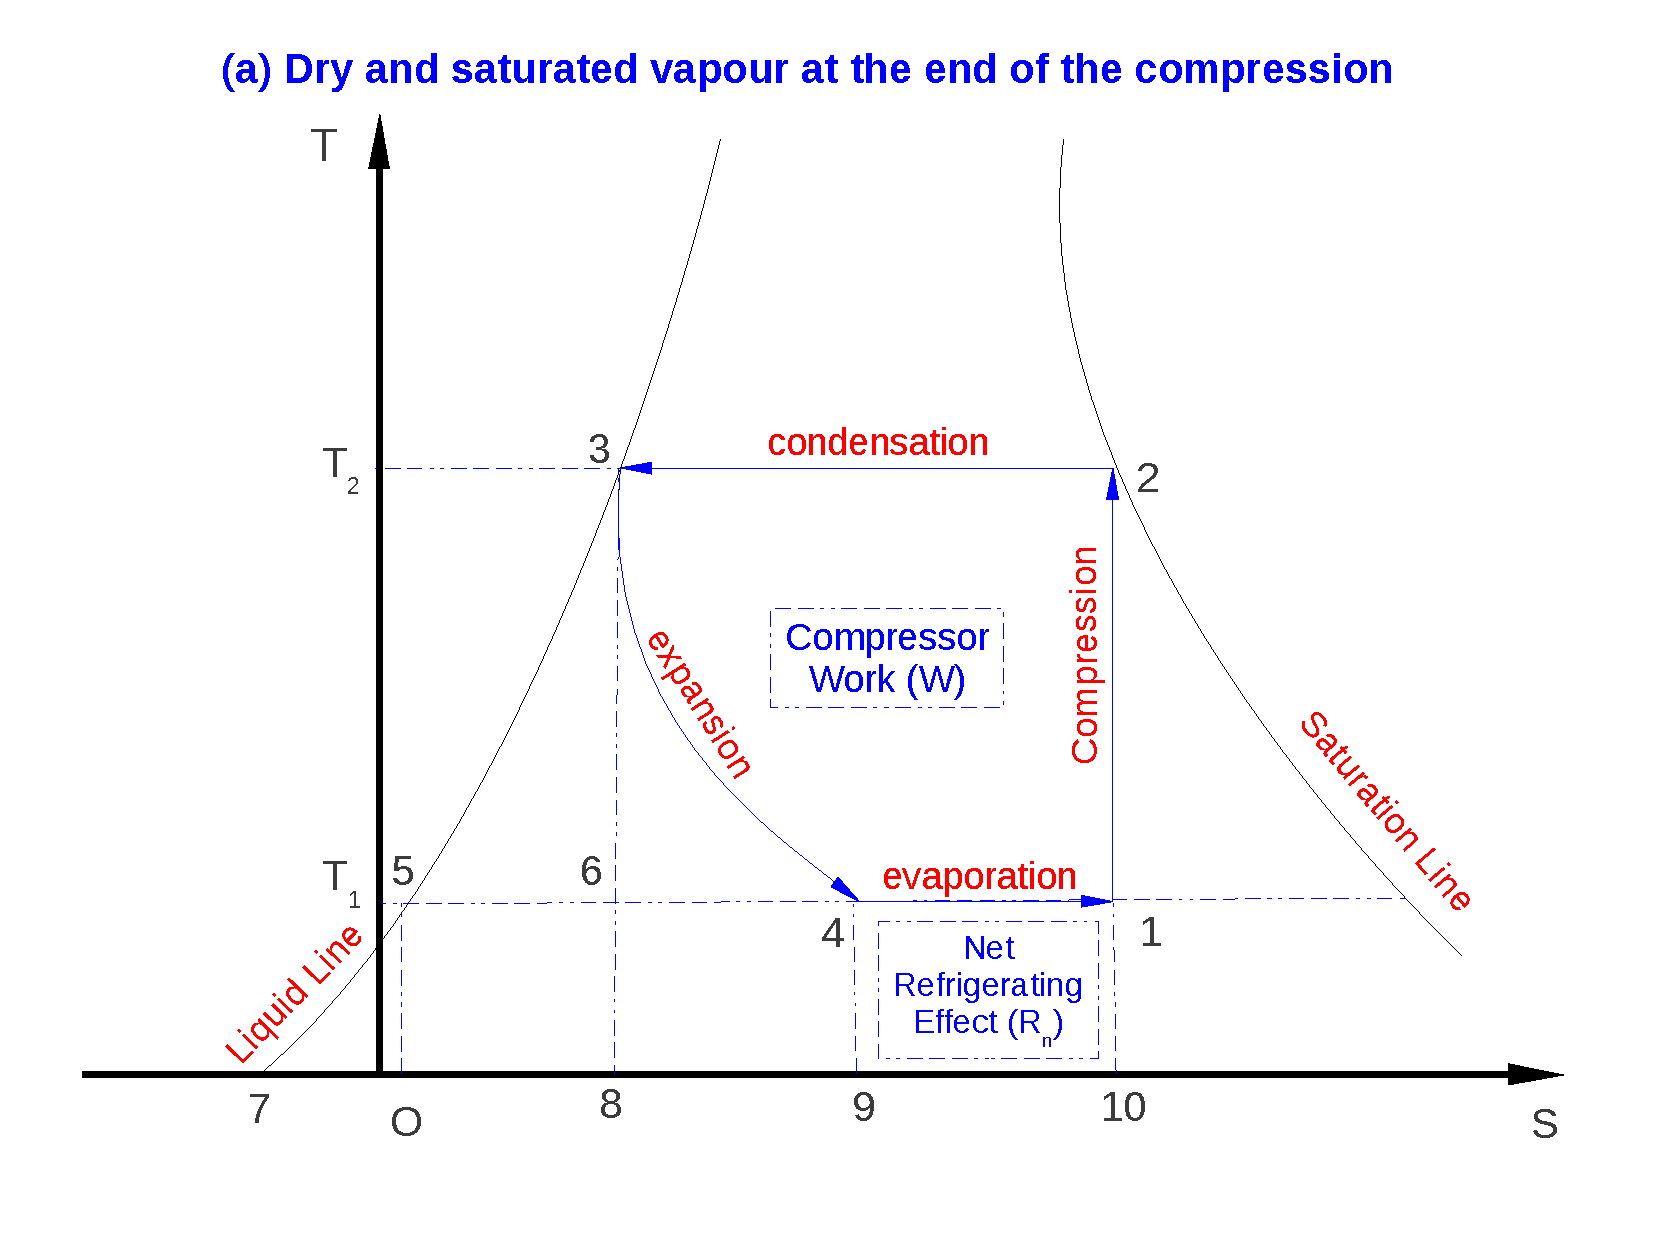
\includegraphics[width=5.4cm,height=2.6cm,clip]{./Pics/Overview_Refrig14}
      \vspace{-.1cm}
      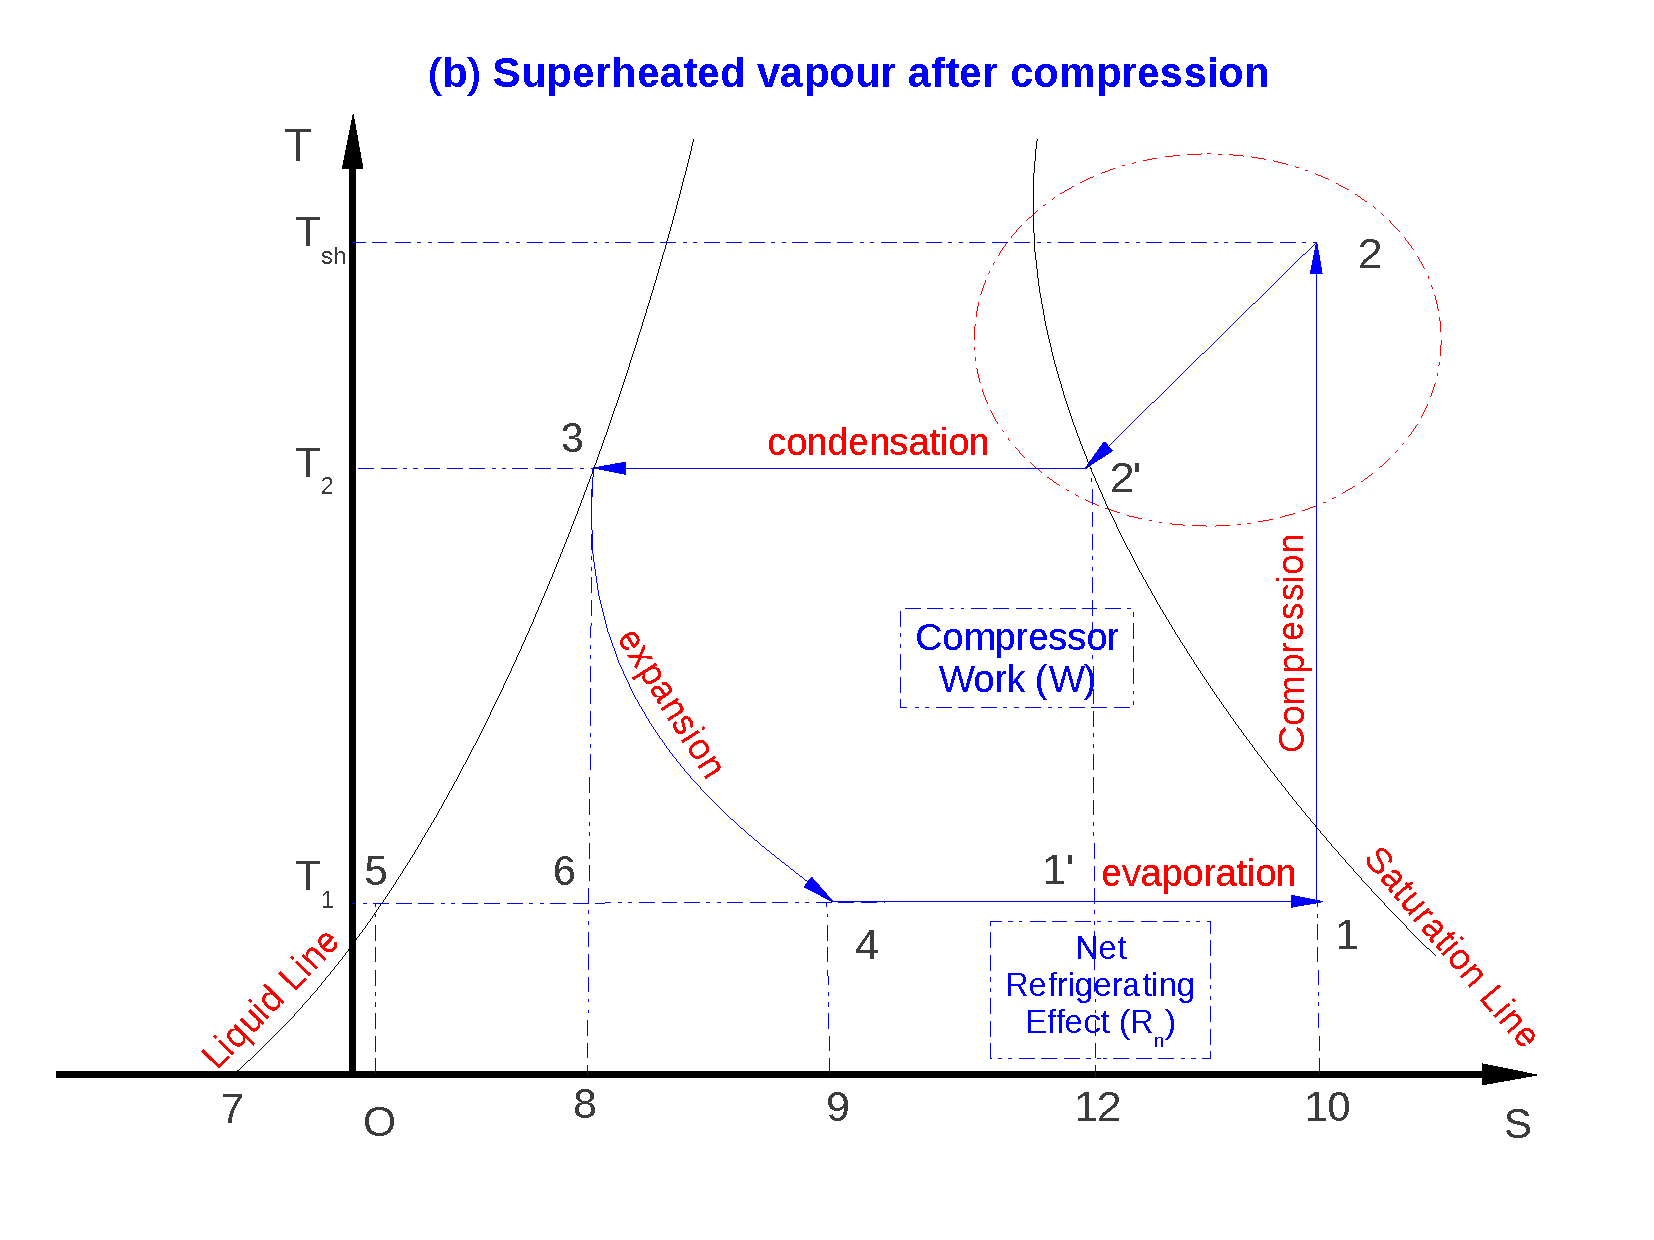
\includegraphics[width=5.4cm,height=2.6cm,clip]{./Pics/Overview_Refrig15}
      \vspace{-.1cm}
      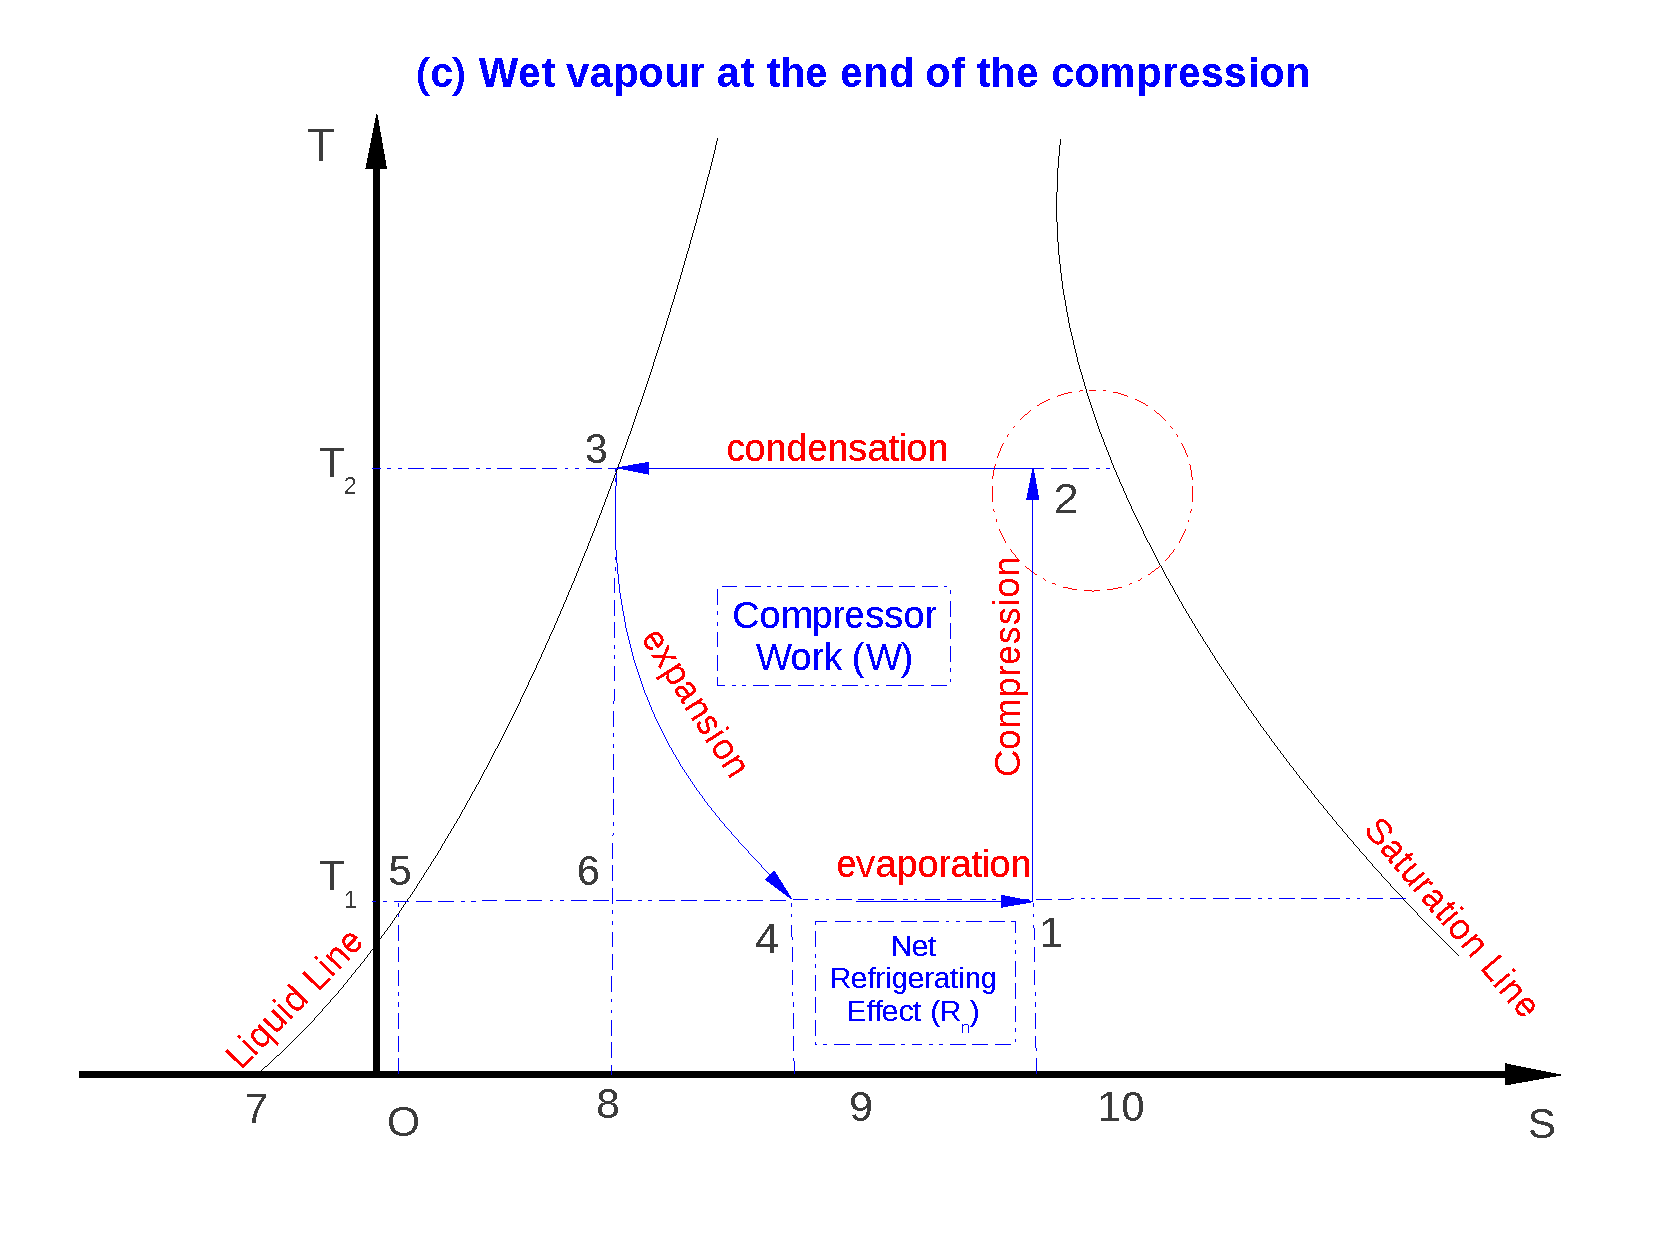
\includegraphics[width=5.4cm,height=2.6cm,clip]{./Pics/Overview_Refrig16}}
   \end{figure}  
  \end{column}  
  \begin{column}[c]{0.35\linewidth}
The \textcolor{blue}{Temperature-Entropy diagram} of the vapour-compression cycle leads to 3 important cases:
   \begin{enumerate}[(a)]
    \item <2-> Vapour is dry and saturated at the end of the compression;
    \item <3-> Vapour is superheated after compression and;
    \item <4-> Vapour is wet after compression.
   \end{enumerate}
  \end{column}  
 \end{columns}
\end{frame}




%%%
%%% Slide
%%%
\begin{frame}
 \frametitle{Thermal Analysis: (a) Dry and Saturated Vapour at the end of the compression}
 \begin{columns}
  \begin{column}[c]{0.55\linewidth}
   \begin{figure}%
     \vbox{
      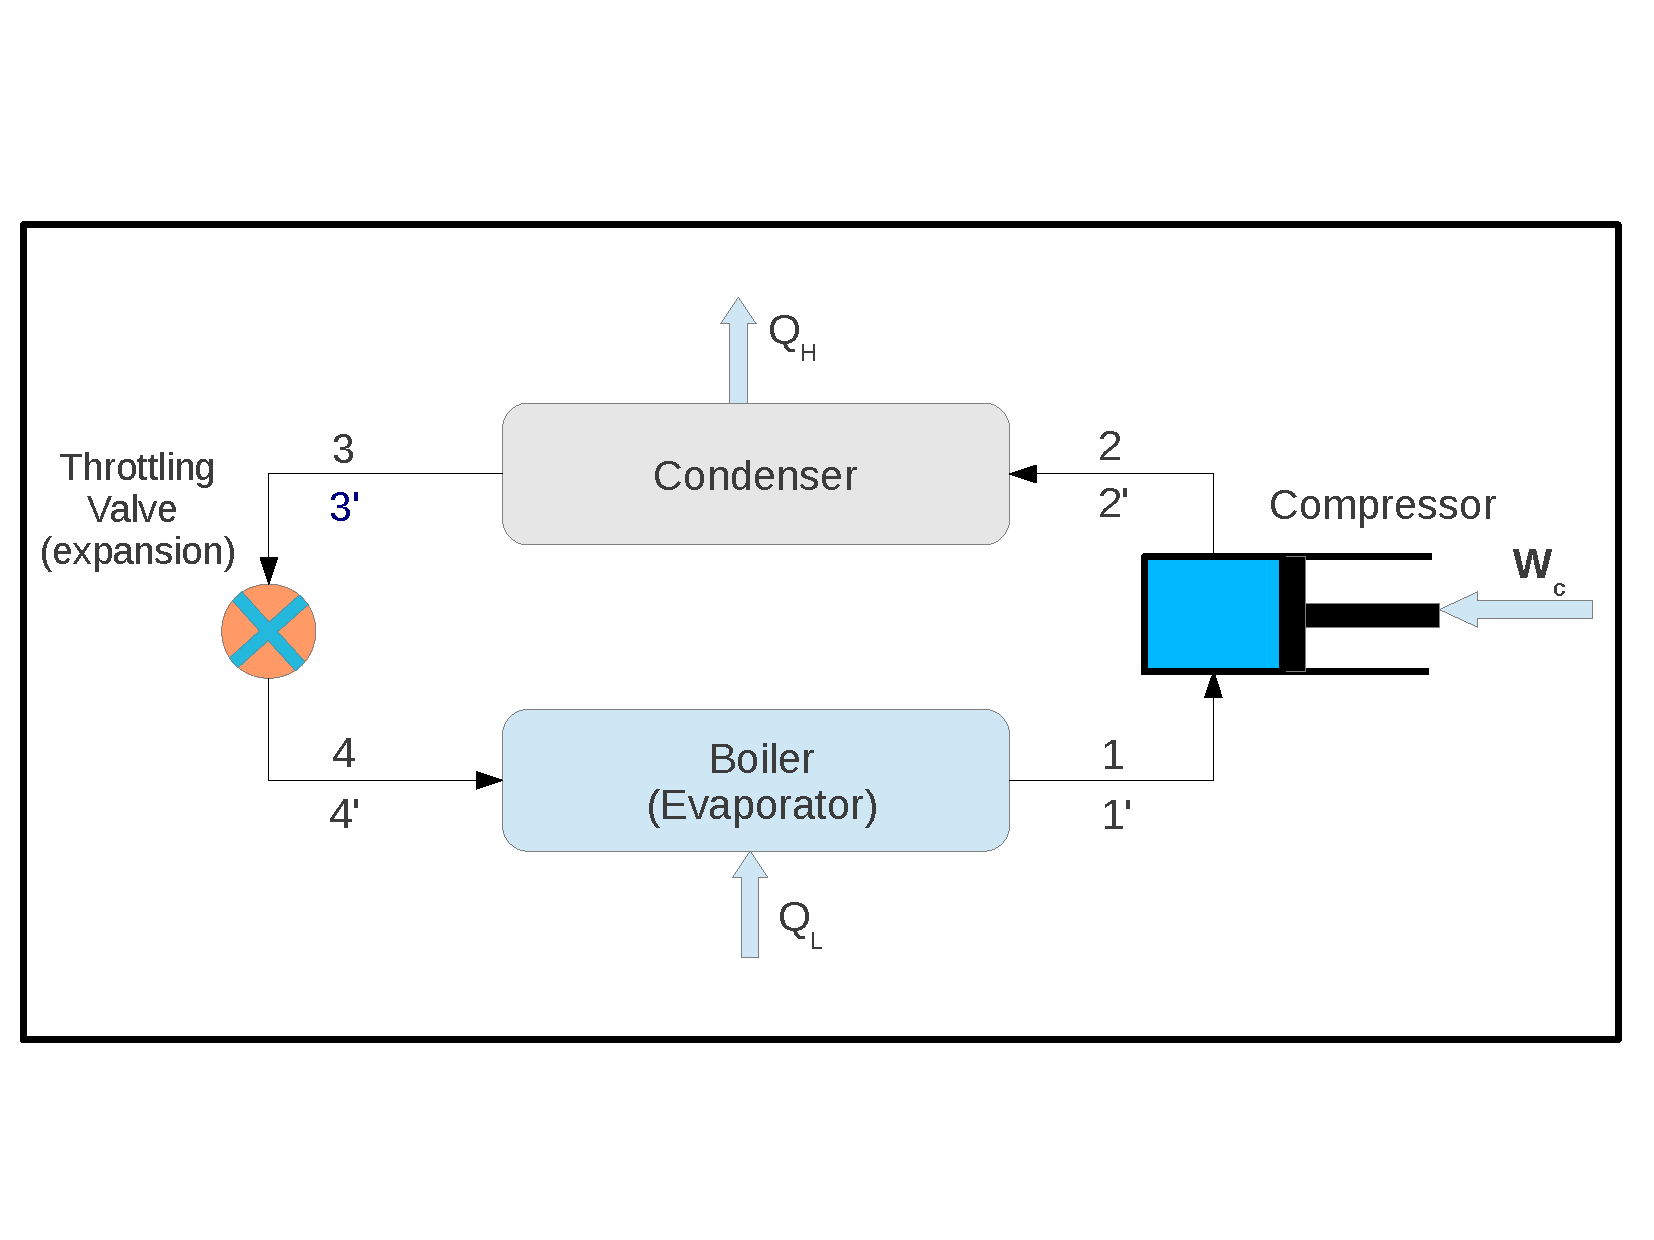
\includegraphics[width=5.cm,height=3.5cm,clip]{./Pics/Overview_Refrig12}
      \vspace{-.6cm}
      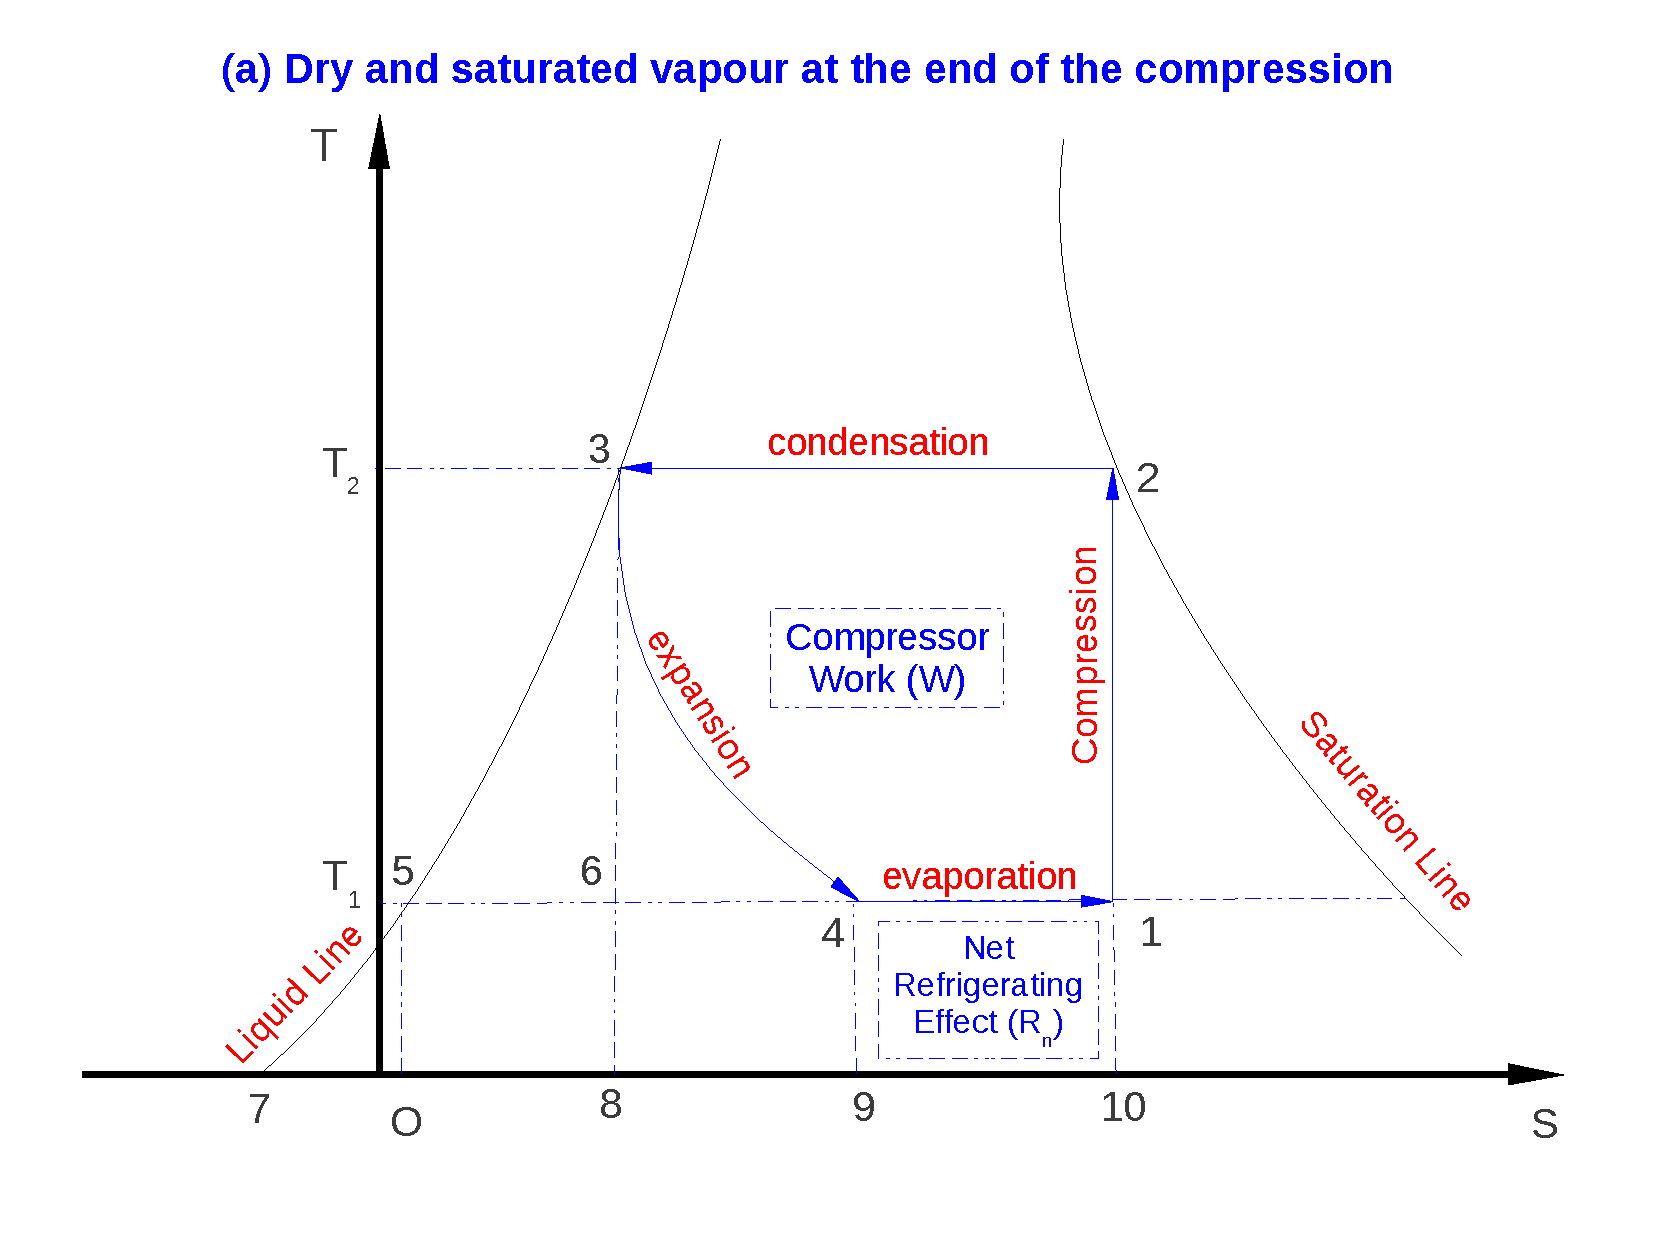
\includegraphics[width=5.5cm,height=4.cm,clip]{./Pics/Overview_Refrig14}}
   \end{figure}  
  \end{column}  
  \begin{column}[c]{0.45\linewidth}
   We can review the cycle as:
   \begin{enumerate}[(a)]
    \item <1-> \textcolor{blue}{1-2}: \textcolor{red}{Isentropic} compression;
    \item <2-> \textcolor{blue}{2-3}: Heat rejection (condenser);
    \item <3-> \textcolor{blue}{3-4}: \textcolor{red}{Isenthalpic} expansion (throttling valve) and;
    \item <4-> \textcolor{blue}{4-1}: Heat absorption (evaporator or refrigerated space). 
   \end{enumerate}
  \end{column}  
 \end{columns}
\end{frame}



%%%
%%% Slide
%%%
\begin{frame}
 \frametitle{Thermal Analysis: (a) Dry and Saturated Vapour at the end of the compression}
 \begin{columns}
  \begin{column}[c]{0.35\linewidth}
   \begin{figure}%
     \vbox{
      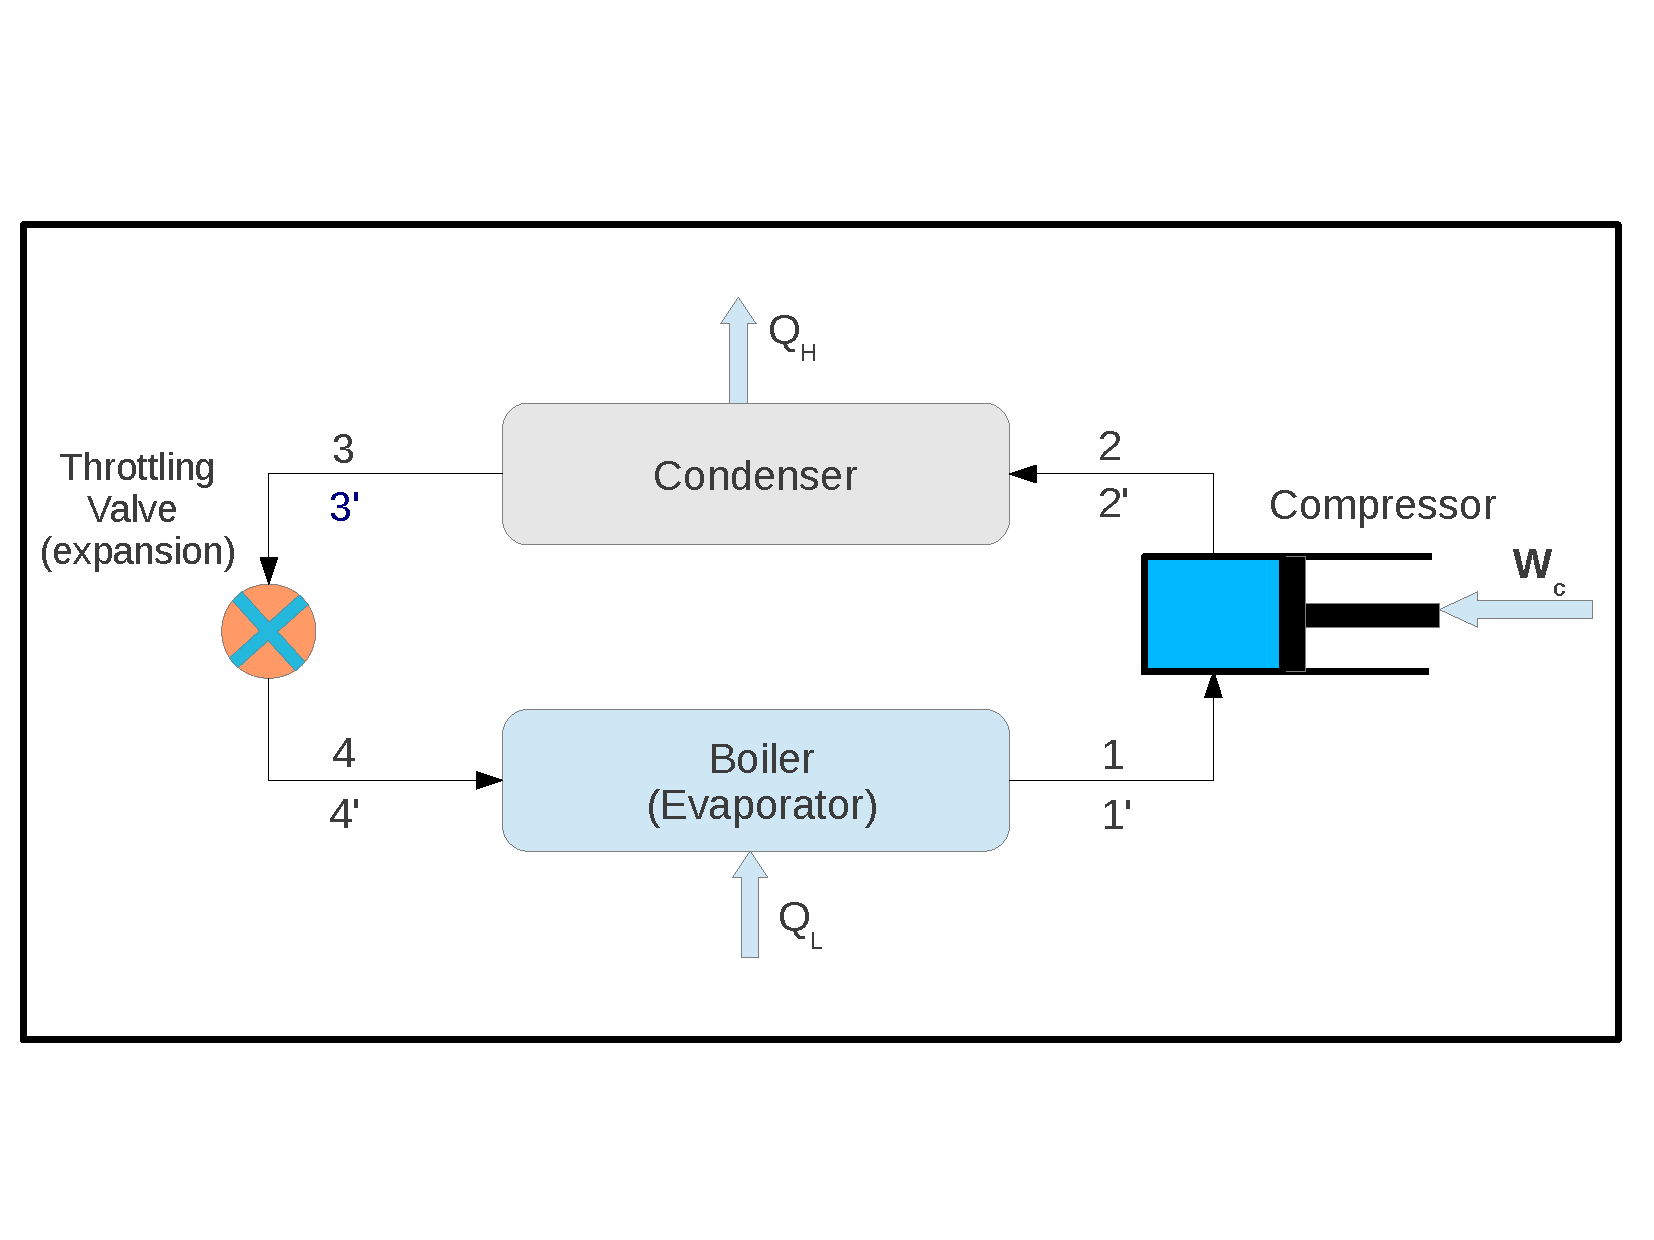
\includegraphics[width=3.5cm,height=3.5cm,clip]{./Pics/Overview_Refrig12}
      \vspace{-.6cm}
      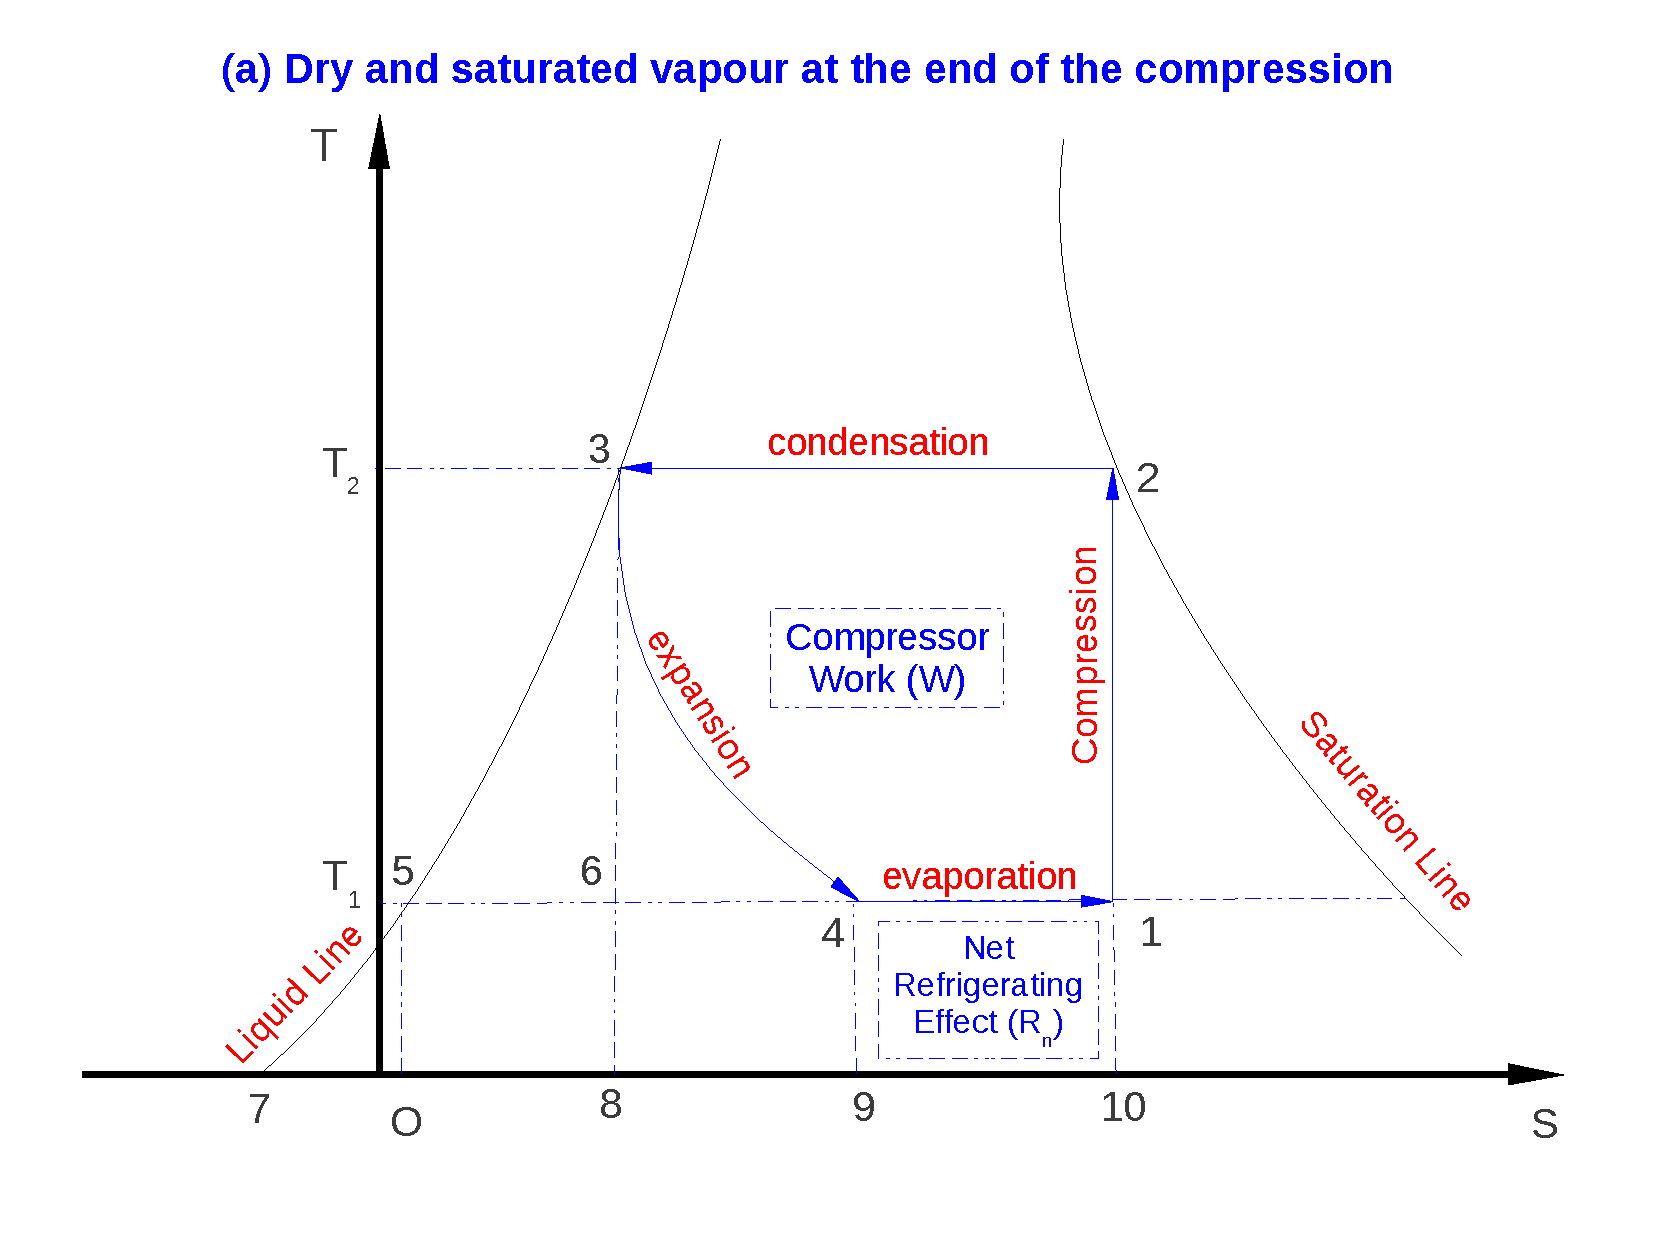
\includegraphics[width=4.cm,height=4.cm,clip]{./Pics/Overview_Refrig14}}
   \end{figure}  
  \end{column}  
  \begin{column}[c]{0.65\linewidth}
   \begin{enumerate}[(a)]
    \item <1-> \textcolor{blue}{Work done} in the cycle is represented by the area within \textcolor{blue}{1-2-3-5-1} on $TS$ diagram:
      \begin{eqnarray}
       \textcolor{blue}{W_{\text{compressor}}} &=& \mathcal{A}_{1-2-3-5-1} \nonumber \\
         &=& \textcolor{blue}{H_{2}-H_{1}}\;\;\text{ with } H_{2} = H_{g}\left(T_{2}\right) \nonumber
      \end{eqnarray}
    \item <2-> \textcolor{blue}{Refrigeration effect} (or heat extracted) in the evaporator is represented by the area within \textcolor{blue}{1-4-9-10-1}:
      \begin{displaymath}
       \textcolor{blue}{R_{n}} = Q_{\text{extract}} = \mathcal{A}_{1-4-9-10-1} = \textcolor{blue}{H_{1}-H_{4}}
      \end{displaymath}
   \end{enumerate}
  \end{column}  
 \end{columns}
\end{frame}


%%%
%%% Slide
%%%
\begin{frame}
 \frametitle{Thermal Analysis: (a) Dry and Saturated Vapour at the end of the compression}
 \begin{columns}
  \begin{column}[c]{0.35\linewidth}
   \begin{figure}%
     \vbox{
      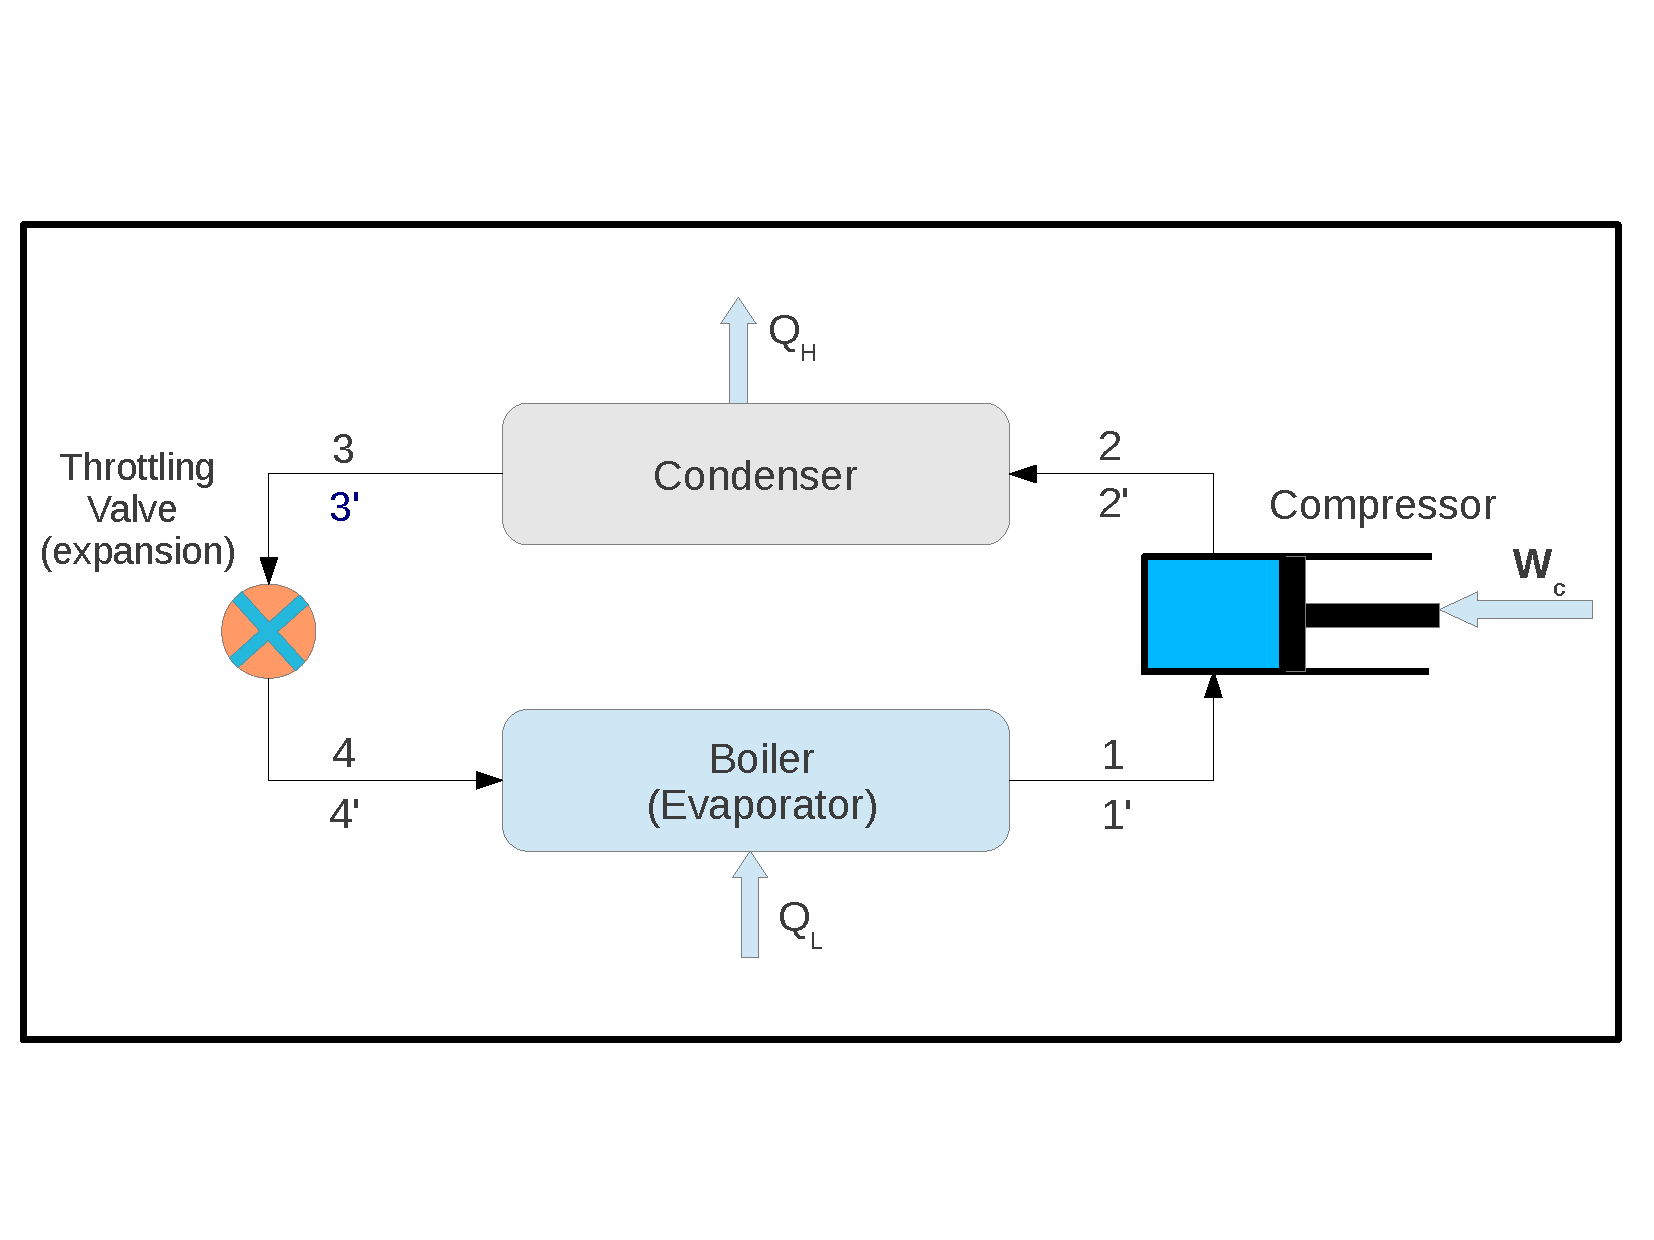
\includegraphics[width=3.5cm,height=3.5cm,clip]{./Pics/Overview_Refrig12}
      \vspace{-.6cm}
      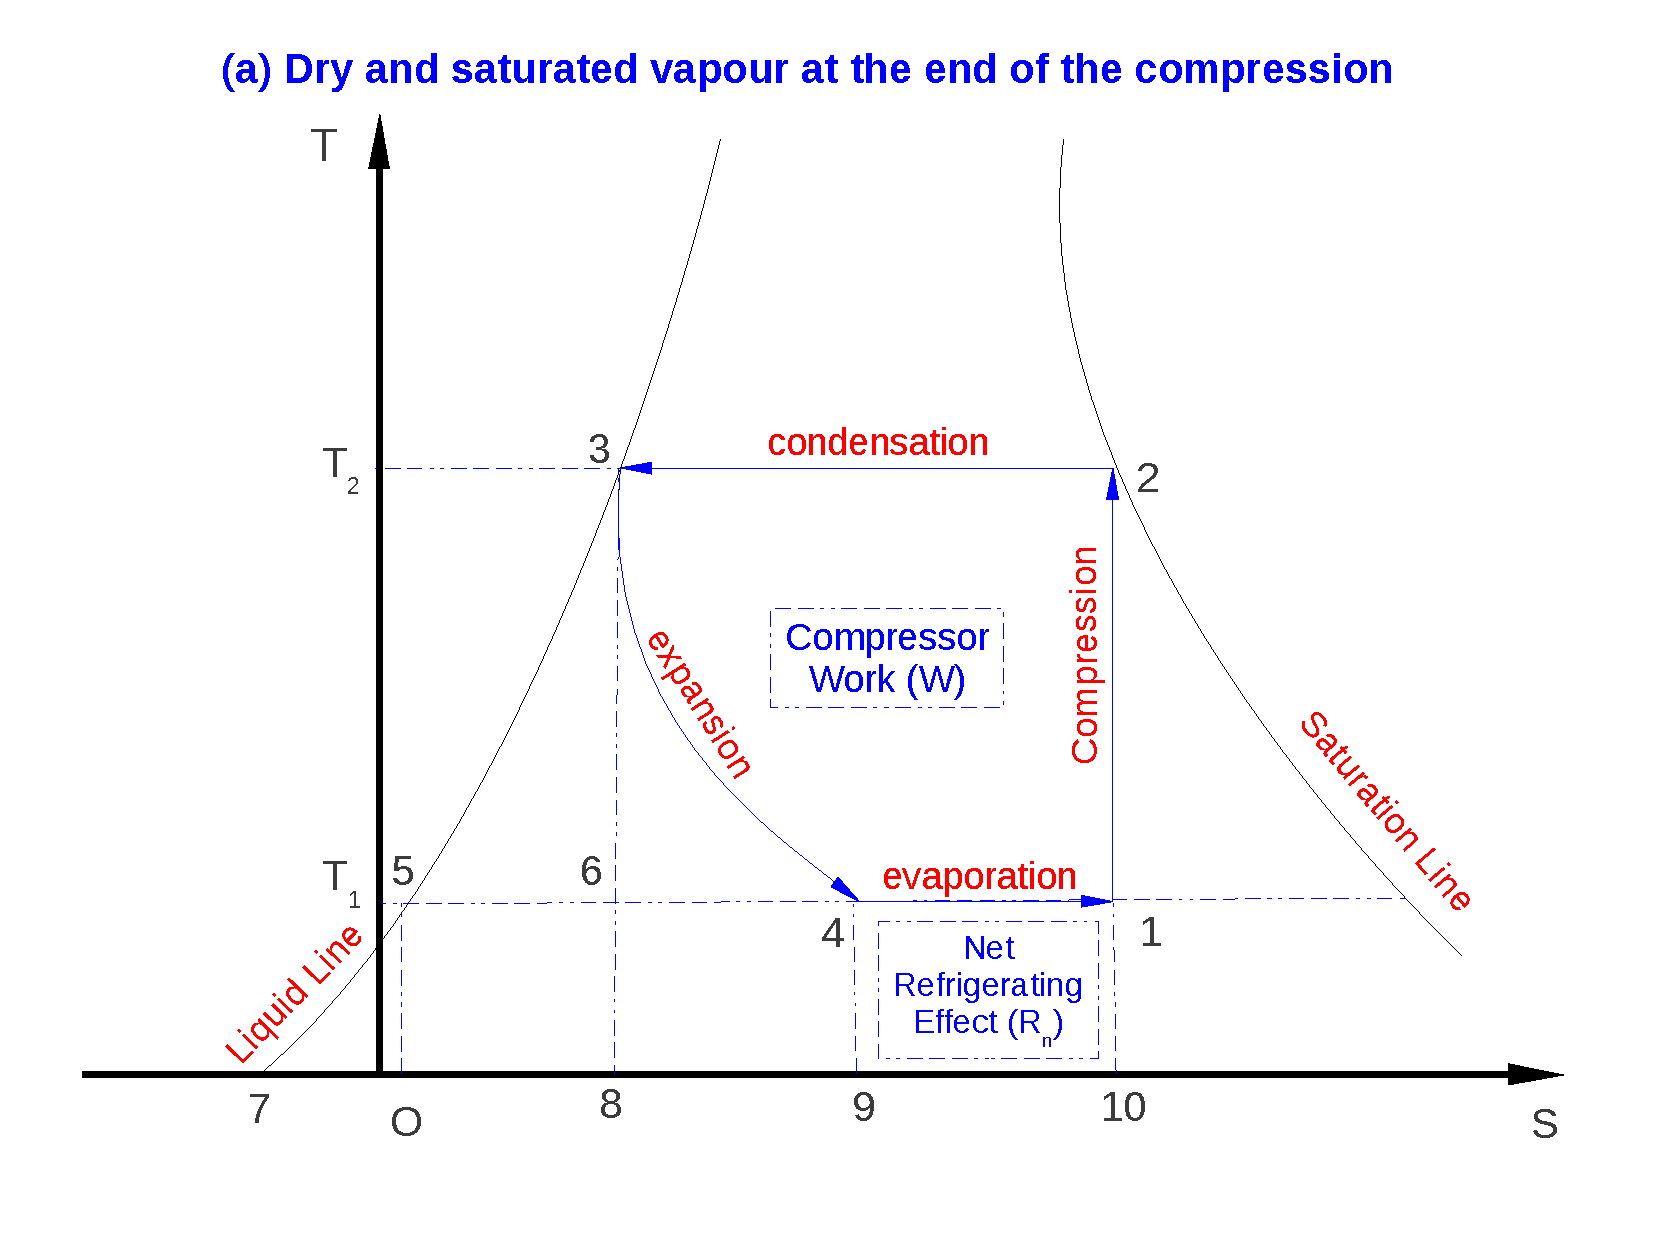
\includegraphics[width=4.cm,height=4.cm,clip]{./Pics/Overview_Refrig14}}
   \end{figure}  
  \end{column}  
  \begin{column}[c]{0.65\linewidth}
   \begin{enumerate}[(a)]
    \item <1-> The \textcolor{blue}{Coefficient of Performance (COP)} is given by
      \begin{displaymath}
       COP= \frc{R_{n}}{W_{\text{compressor}}}=\frc{H_{1}-H_{4}}{H_{2}-H_{1}}
      \end{displaymath}
    \item <2-> During the \textcolor{blue}{throttling expansion (3-4)} the total heat content remains constant, i.e., $H_{4}=H_{3}$, thus
      \begin{displaymath}
       \textcolor{blue}{COP}= \frc{H_{1}-H_{4}}{H_{2}-H_{1}} = \textcolor{blue}{\frc{H_{1}-H_{3}}{H_{2}-H_{1}}}
      \end{displaymath}
   \end{enumerate}
  \end{column}  
 \end{columns}
\end{frame}


%%%
%%% Slide
%%%
\begin{frame}
 \frametitle{Thermal Analysis: (b) Vapour is superheated after compression}
 \begin{columns}
  \begin{column}[c]{0.35\linewidth}
   \begin{figure}%
     \vbox{
      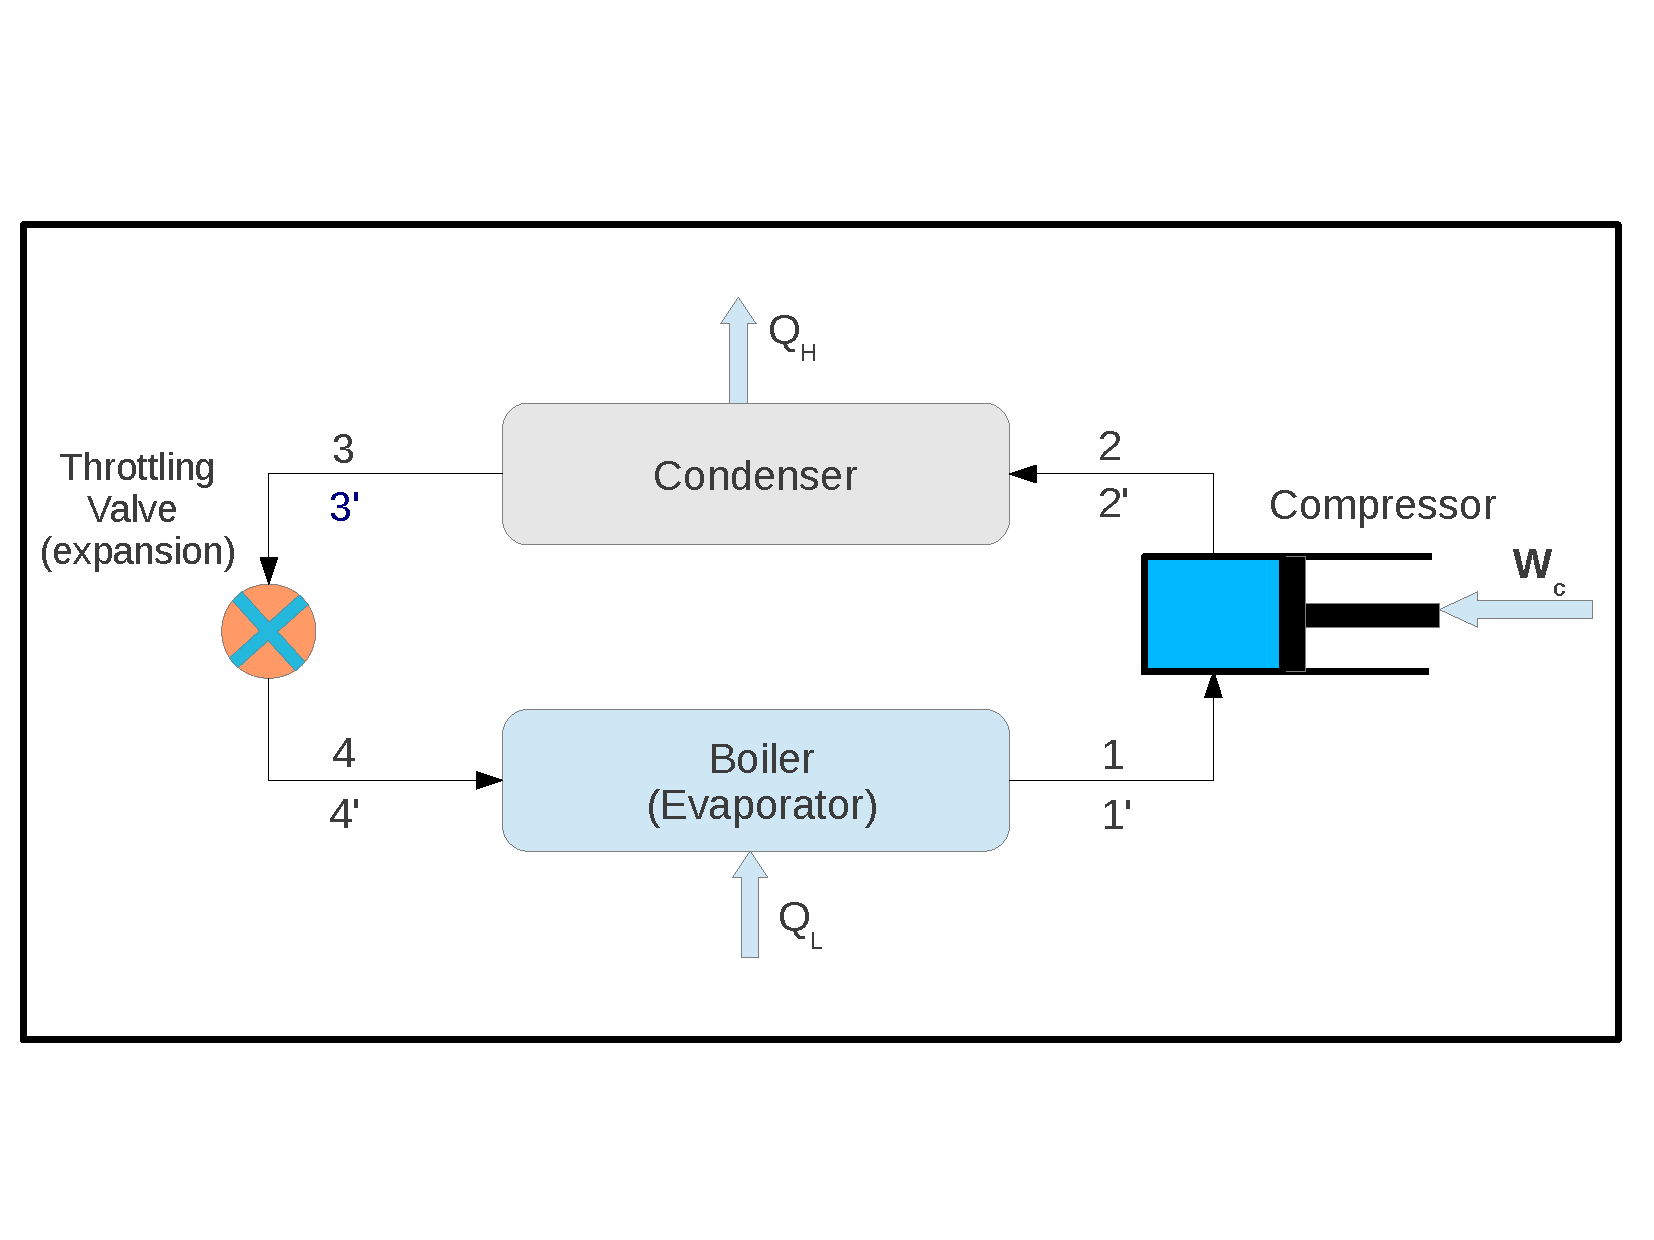
\includegraphics[width=3.5cm,height=3.5cm,clip]{./Pics/Overview_Refrig12}
      \vspace{-.6cm}
      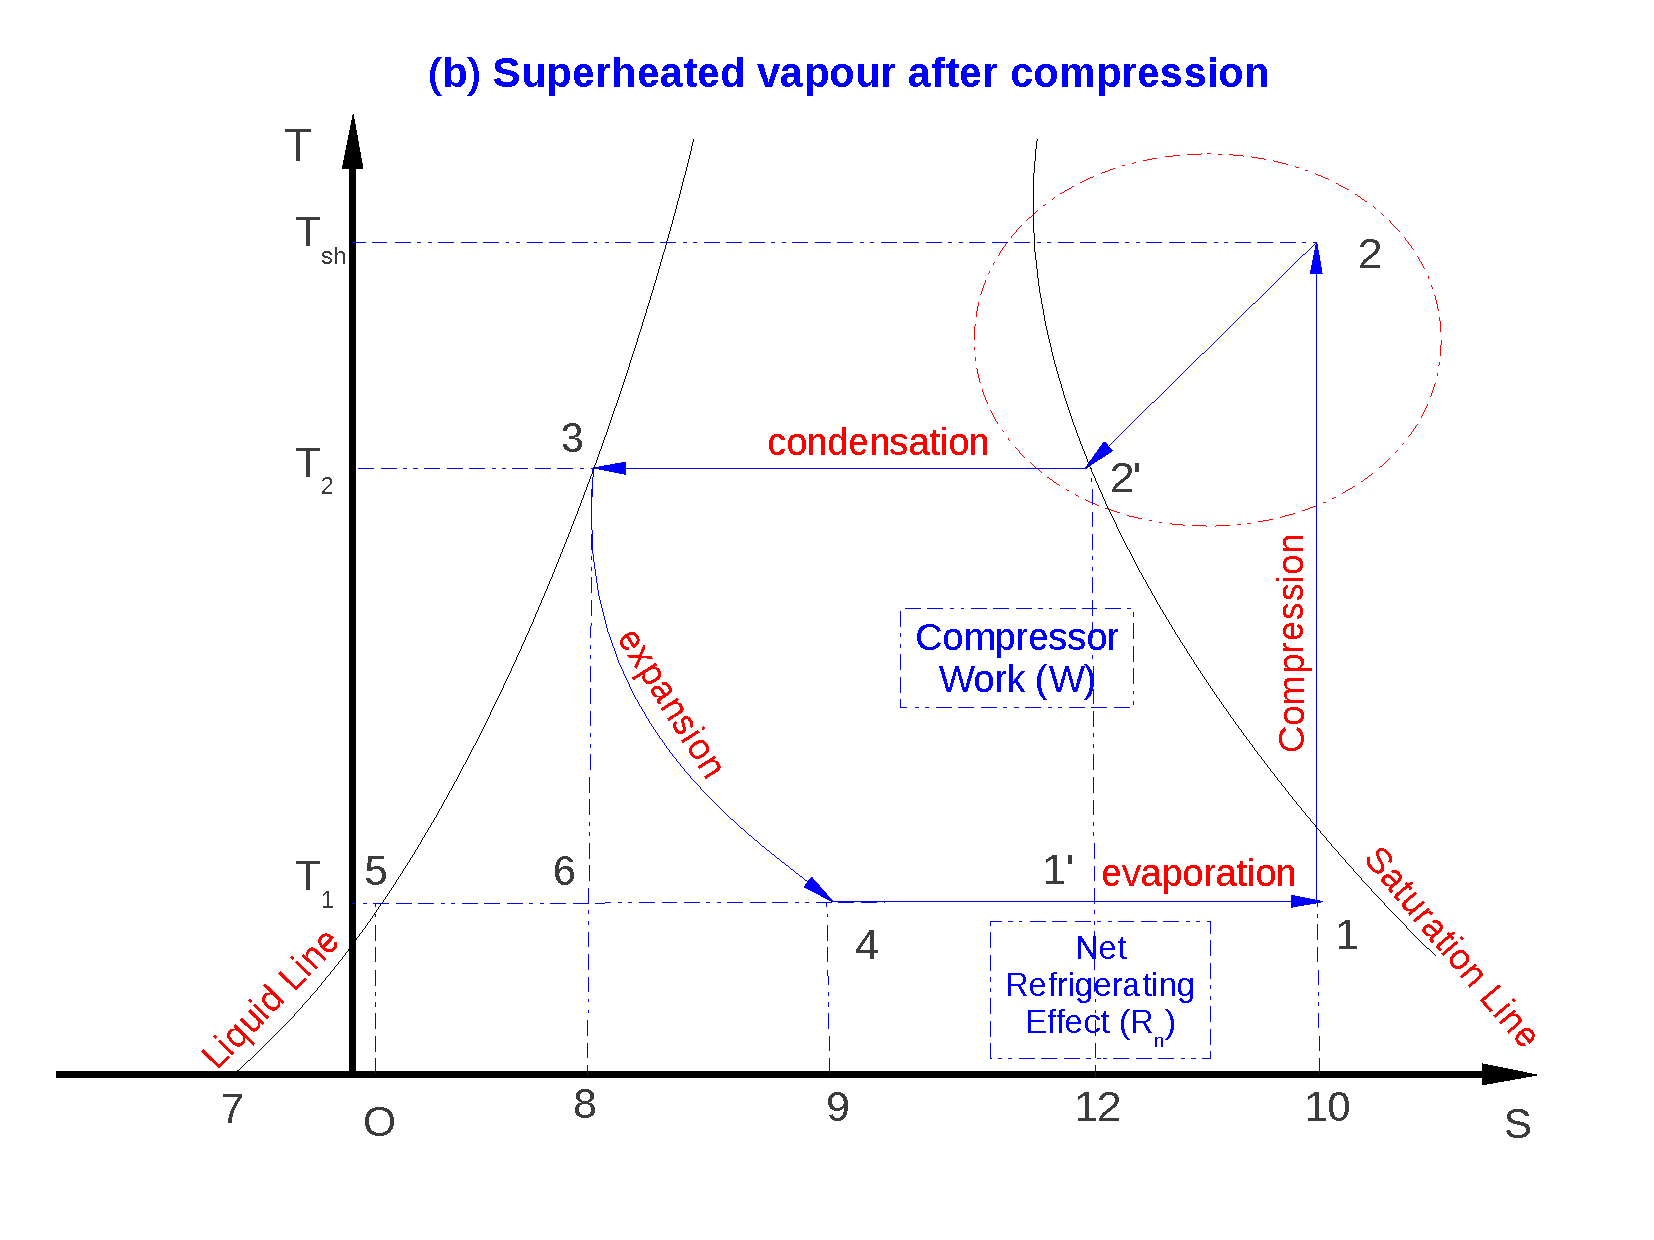
\includegraphics[width=4.cm,height=4.cm,clip]{./Pics/Overview_Refrig15}}
   \end{figure}  
  \end{column}  
  \begin{column}[c]{0.65\linewidth}
   \begin{enumerate}[(a)]
    \item <1-> \textcolor{blue}{Work done} in the cycle is represented by the area within \textcolor{blue}{1-2-2$^{\prime}$-3-5-1$^{\prime}$-1} on $TS$ diagram:
      \begin{eqnarray} 
       \textcolor{blue}{W_{\text{compressor}}} &=& \mathcal{A}_{1-2-2'-3-5-1'-1} \nonumber \\
         &=& \textcolor{blue}{H_{2}-H_{1}} \nonumber
      \end{eqnarray}
    \item <2-> \textcolor{blue}{Refrigeration effect} (or heat extracted) is represented by the area within \textcolor{blue}{1-1'-4-9-10-1}:
      \begin{displaymath}
       \textcolor{blue}{R_{n}} = Q_{\text{extract}} = \mathcal{A}_{1-1'-4-9-10-1} = \textcolor{blue}{H_{1}-H_{4}}
      \end{displaymath}
   \end{enumerate}
  \end{column}  
 \end{columns}
\end{frame}



%%%
%%% Slide
%%%
\begin{frame}
 \frametitle{Thermal Analysis: (b) Vapour is superheated after compression}
 \begin{columns}
  \begin{column}[c]{0.35\linewidth}
   \begin{figure}%
     \vbox{
      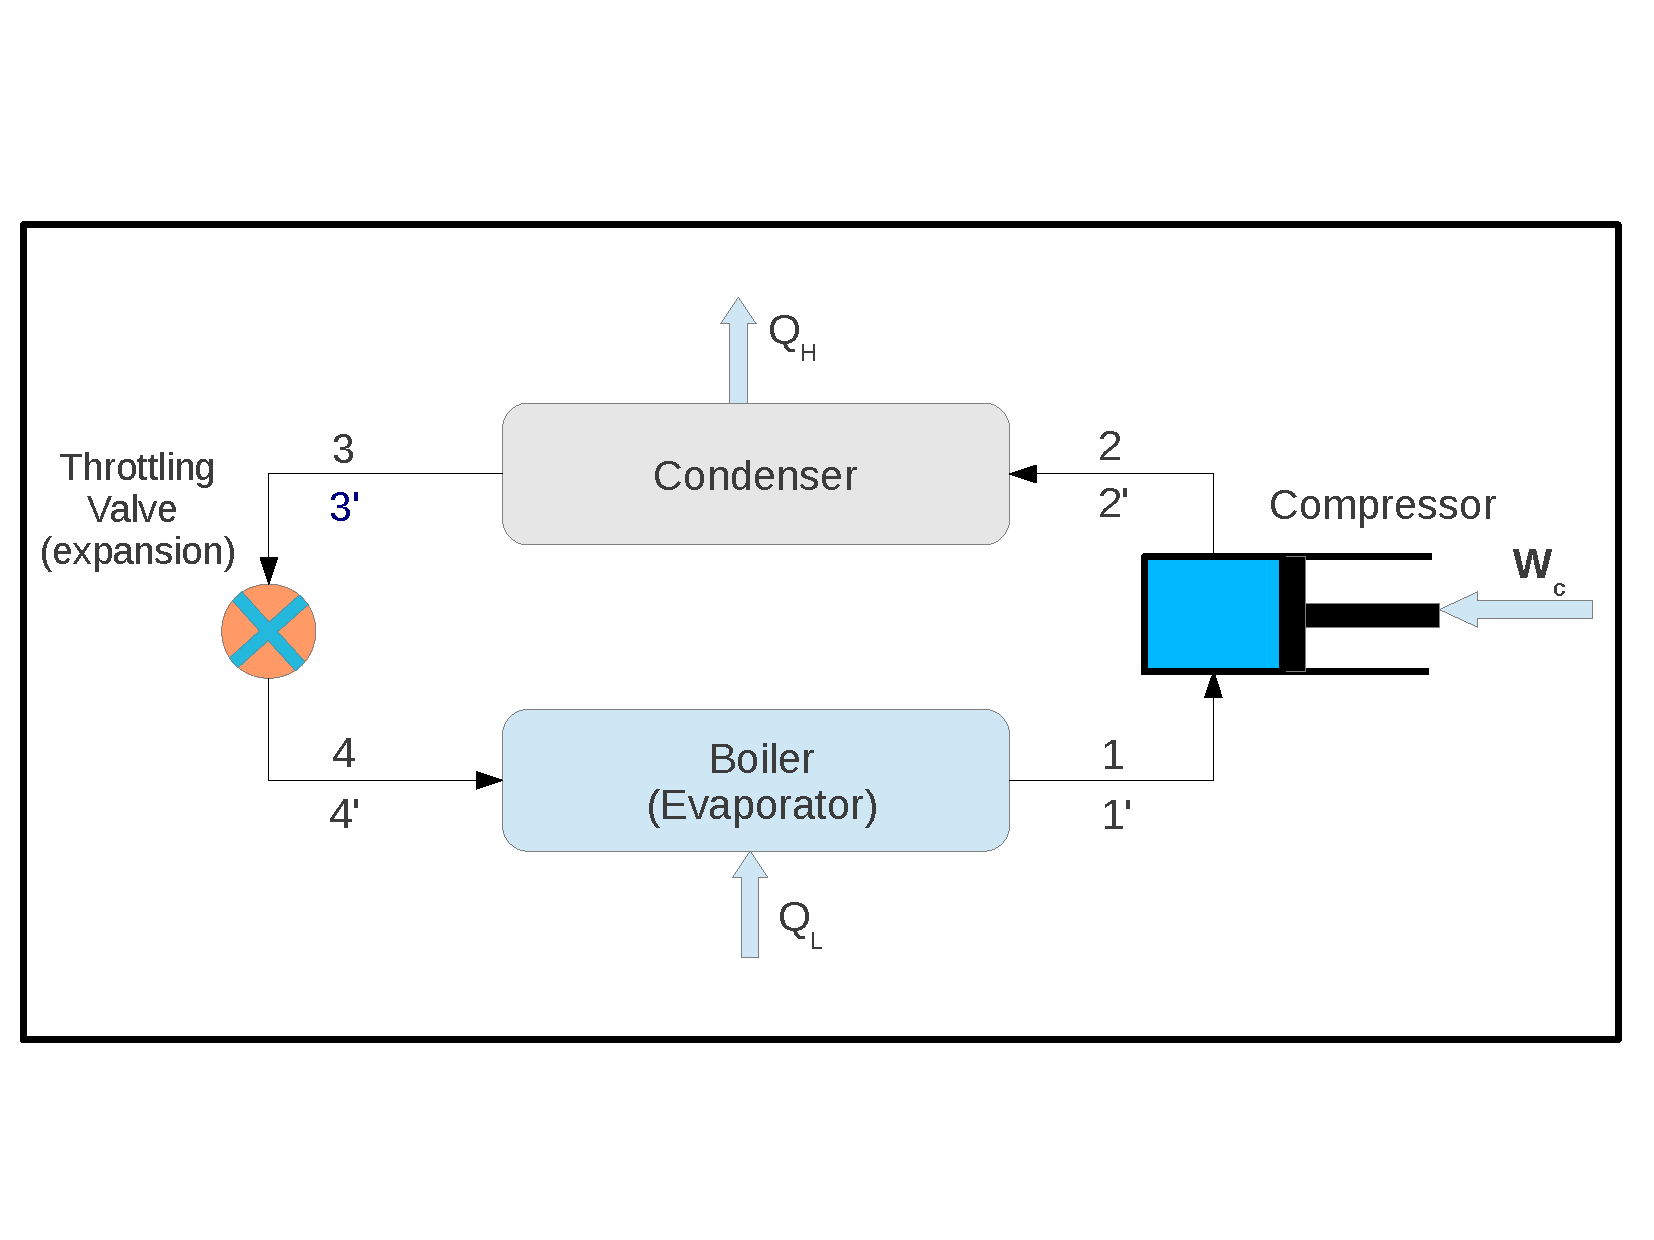
\includegraphics[width=3.5cm,height=3.5cm,clip]{./Pics/Overview_Refrig12}
      \vspace{-.6cm}
      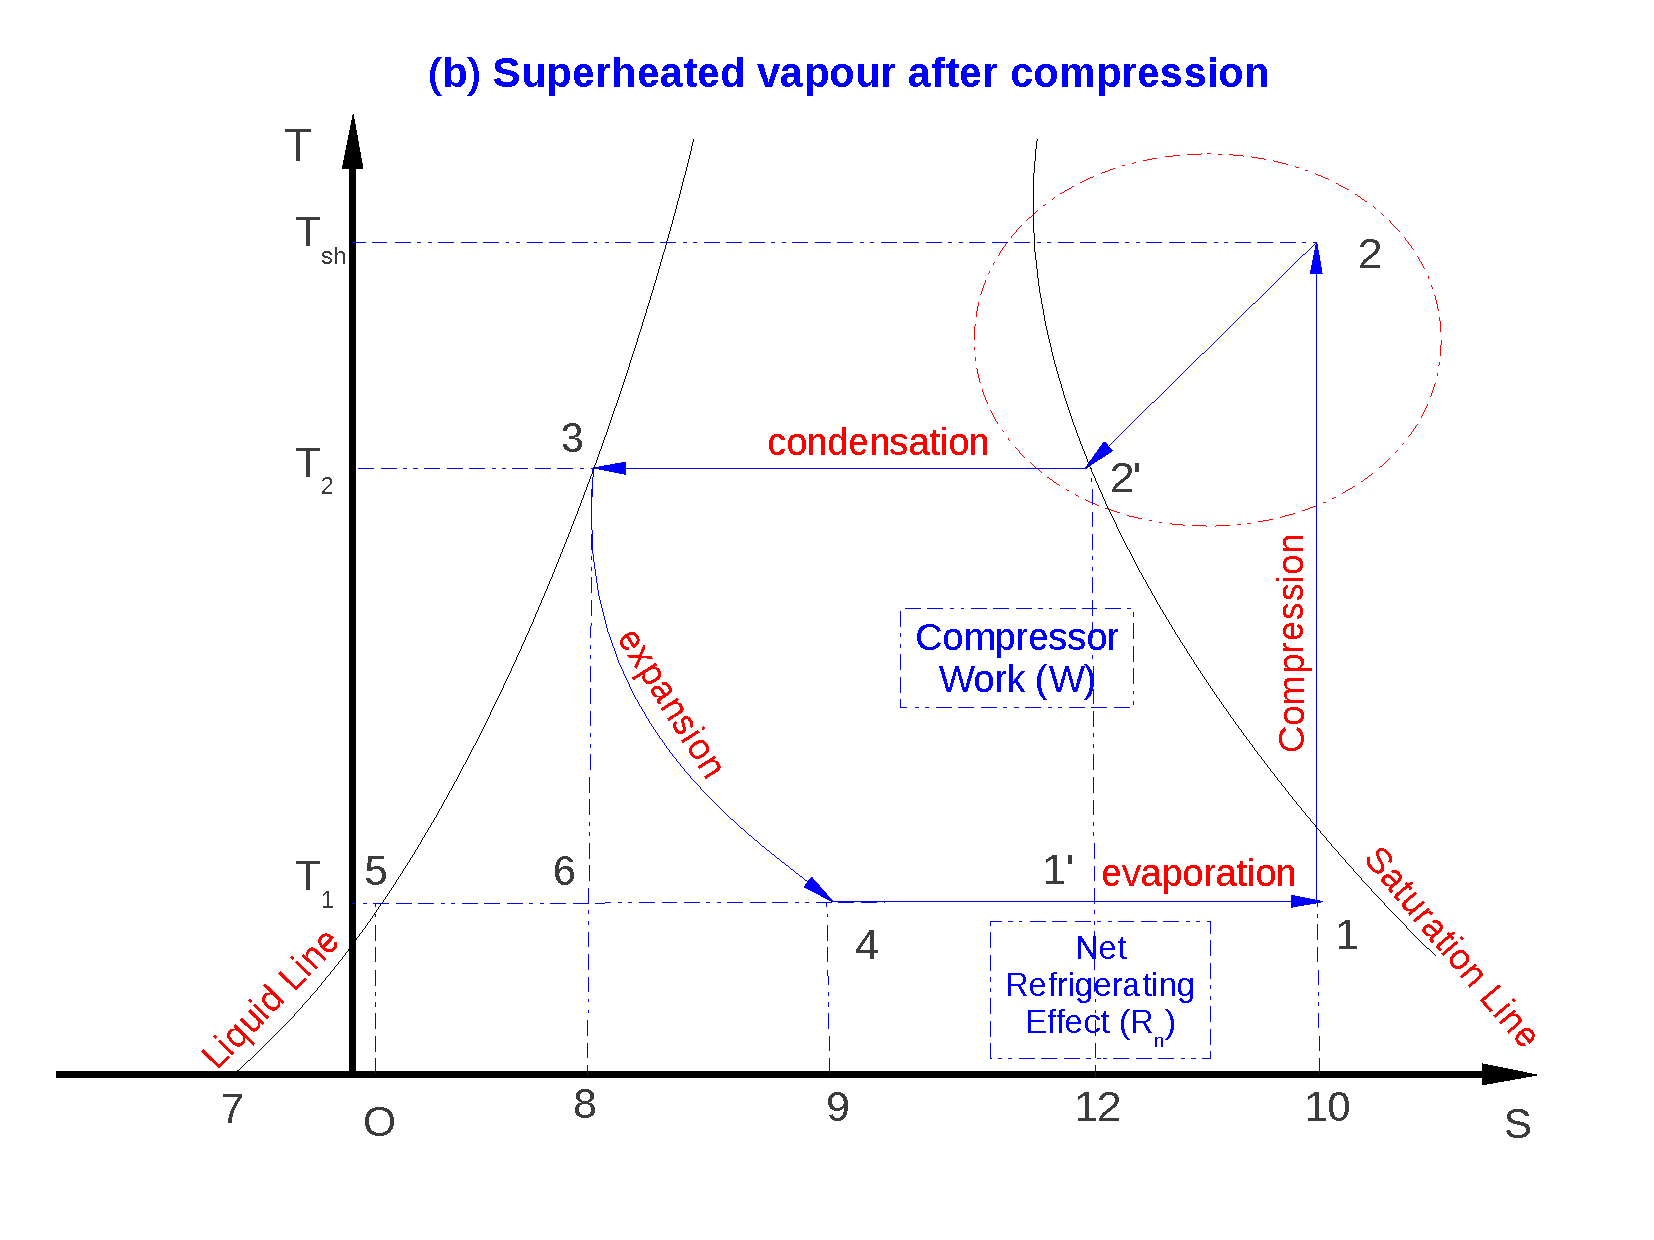
\includegraphics[width=4.cm,height=4.cm,clip]{./Pics/Overview_Refrig15}}
   \end{figure}  
  \end{column}  
  \begin{column}[c]{0.65\linewidth}
   \begin{enumerate}[(a)]
    \item <1-> The \textcolor{blue}{Coefficient of Performance (COP)} is given by
      \begin{displaymath}
       \textcolor{blue}{COP}= \frc{R_{n}}{W_{\text{compressor}}}=\textcolor{blue}{\frc{H_{1}-H_{4}}{H_{2}-H_{1}}}
      \end{displaymath}
    \item <2-> The enthalpy of the superheated fluid at \textcolor{blue}{state 2} is
      \begin{displaymath}
        H_{2} = H_{2'} + C_{p}\left(T_{\text{superheated}}-T_{\text{sat}}\right)
      \end{displaymath}
      Where $H_{2'}$ is the total heat of dry and saturated vapour at \textcolor{blue}{state 2}. $T_{\text{superheated}}=T_{sh}$ and $T_{\text{sat}}=T_{2}$
   \end{enumerate}
  \end{column}  
 \end{columns} 
\end{frame}




%%%
%%% Slide
%%%
\begin{frame}
 \frametitle{Thermal Analysis: (c) Vapour is wet after compression.}
 \begin{columns}
  \begin{column}[c]{0.35\linewidth}
   \begin{figure}%
     \vbox{
      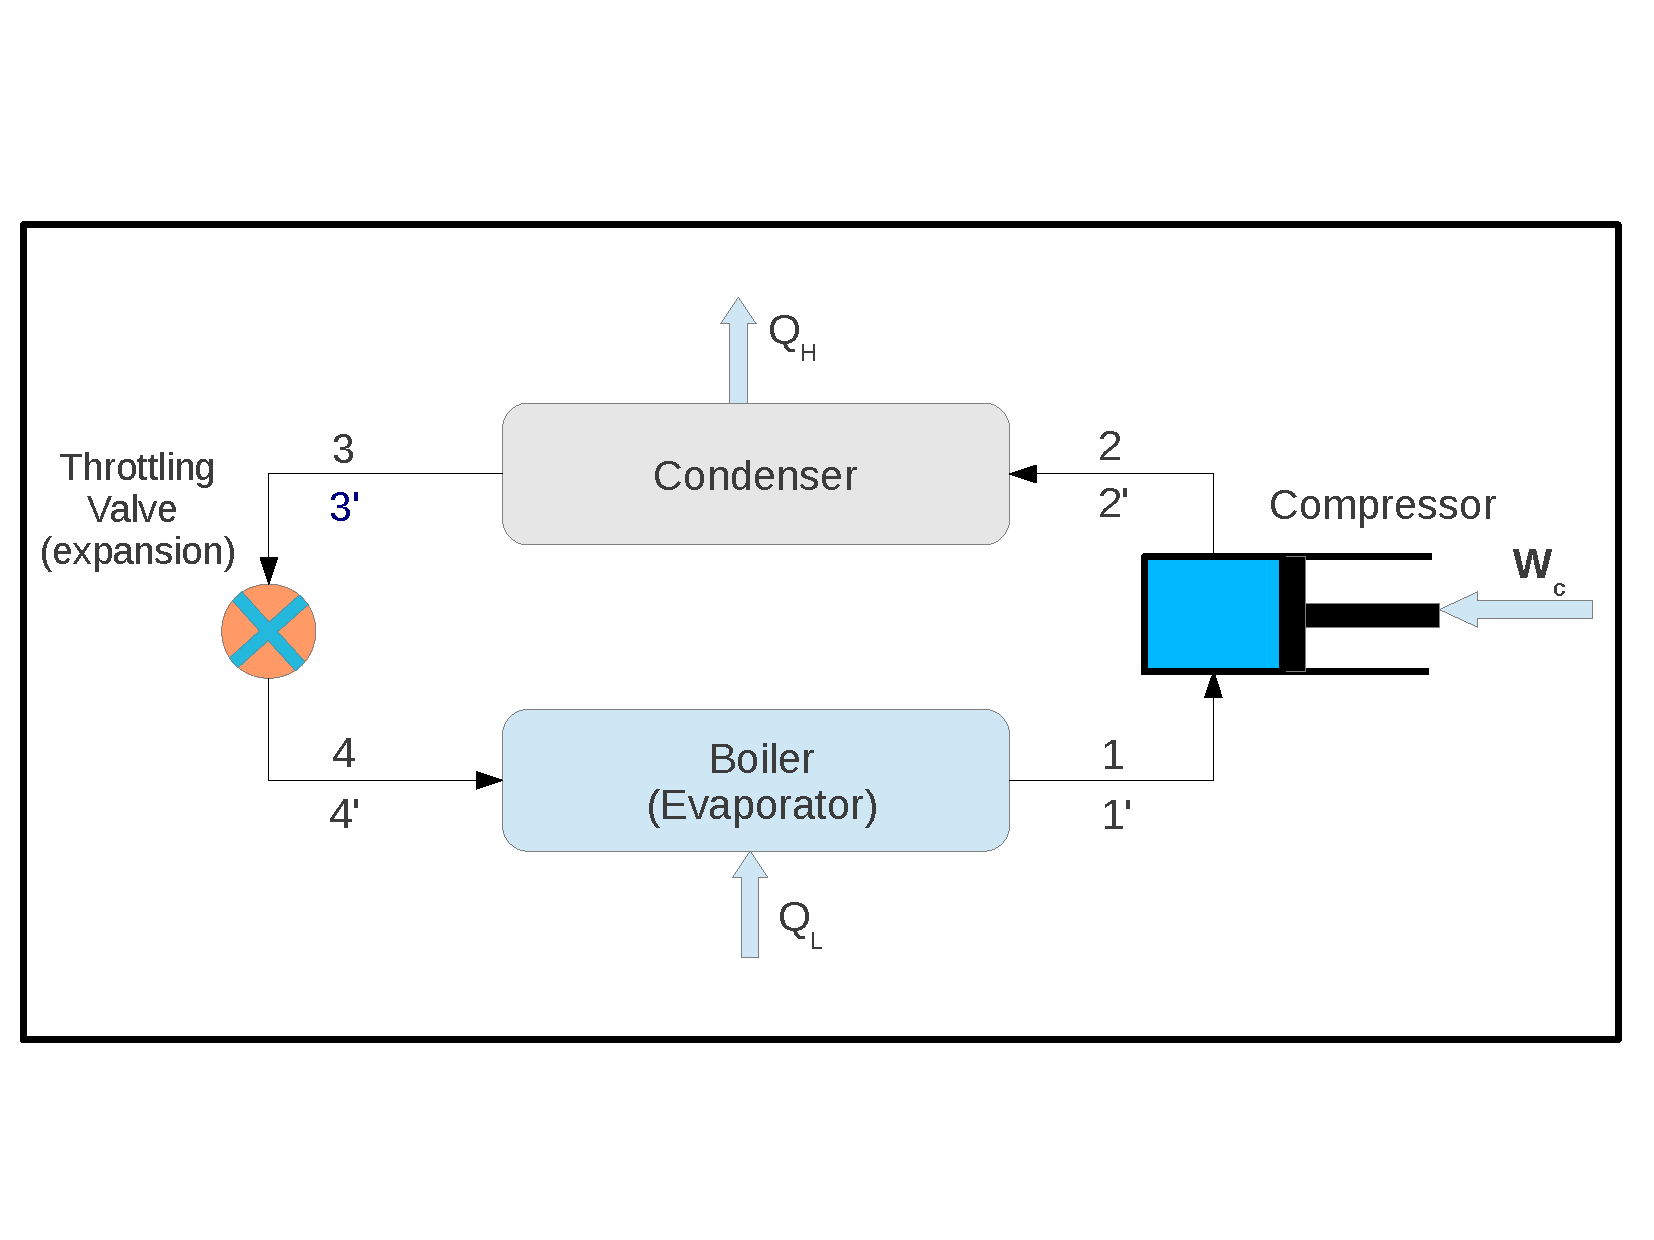
\includegraphics[width=3.5cm,height=3.5cm,clip]{./Pics/Overview_Refrig12}
      \vspace{-.6cm}
      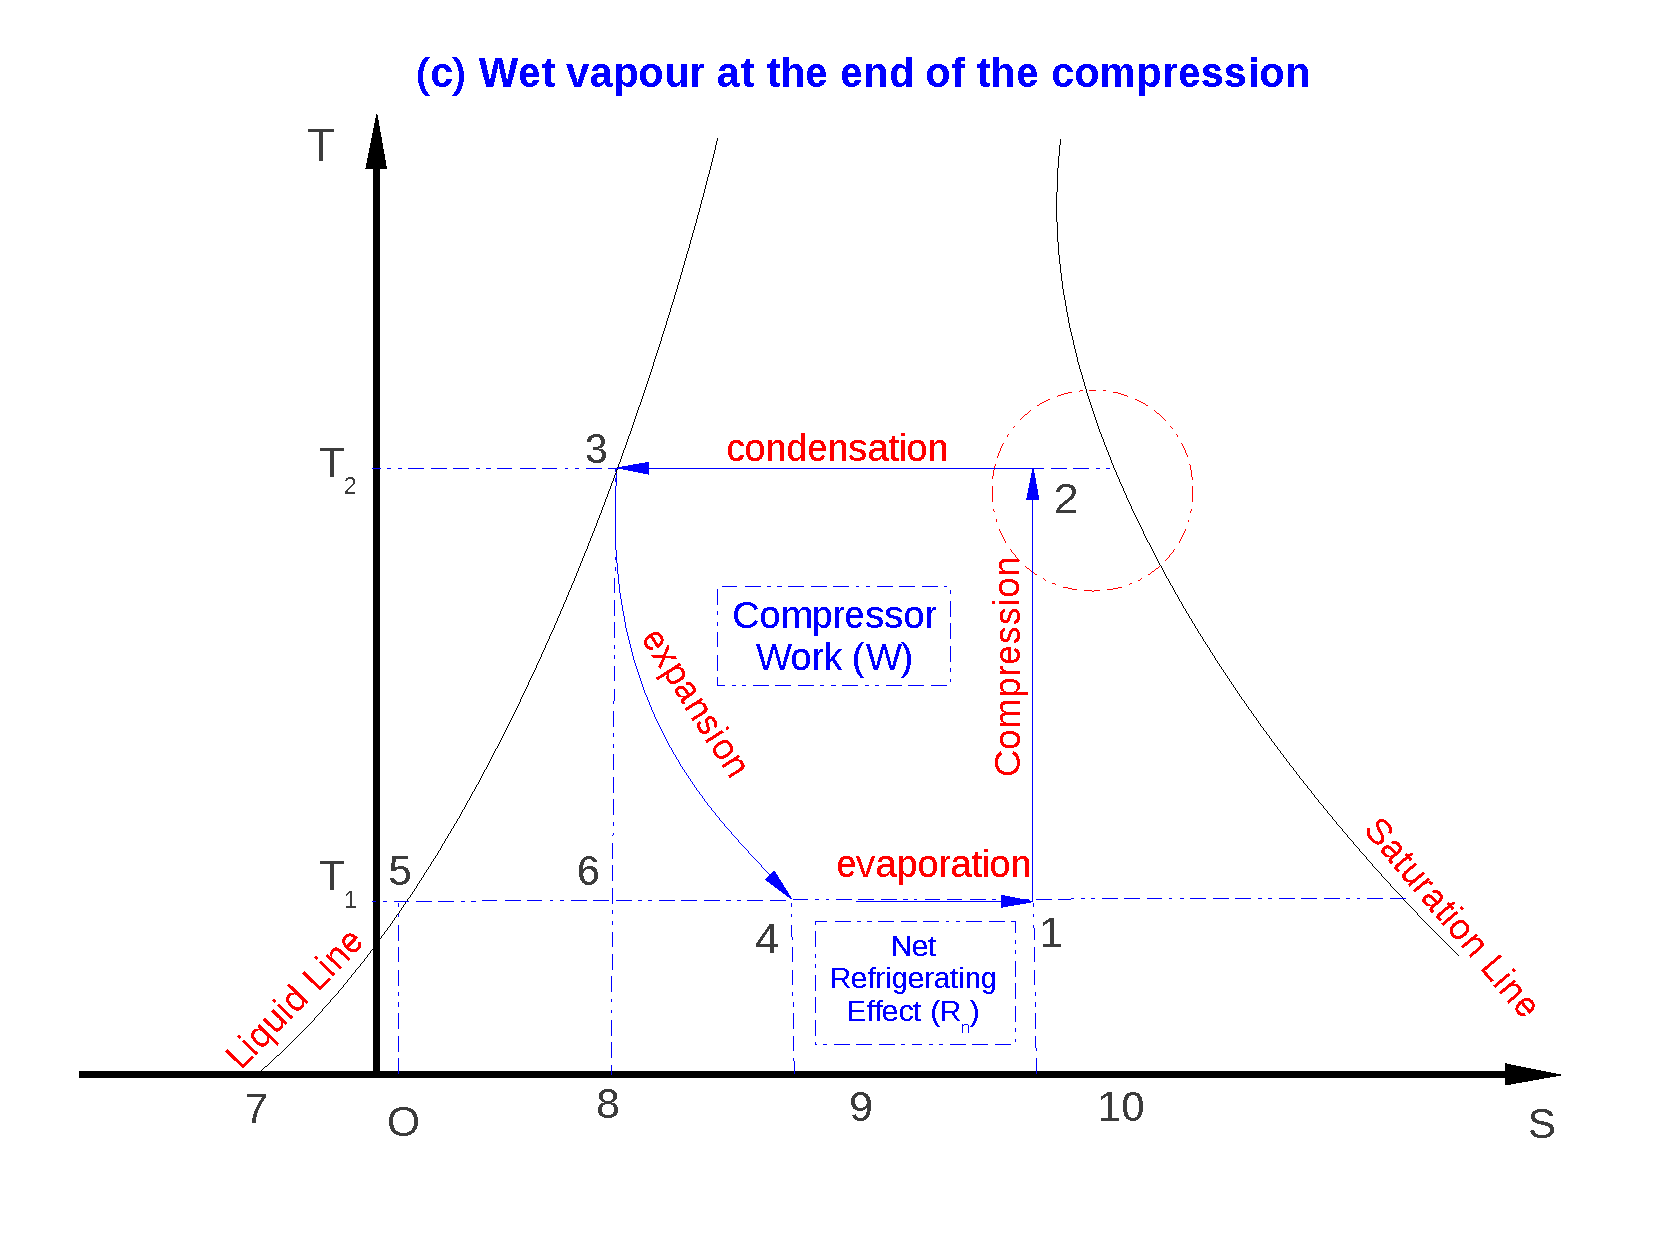
\includegraphics[width=4.cm,height=4.cm,clip]{./Pics/Overview_Refrig16}}
   \end{figure}  
  \end{column}  
  \begin{column}[c]{0.65\linewidth}
   \begin{enumerate}[(a)]
    \item <1-> In this case, the compression process results in wet vapour formation at state 2;
    \item <2-> \textcolor{blue}{Work done} in the cycle is represented by the area within \textcolor{blue}{1-2--3-5-1} on $TS$ diagram:
      \begin{eqnarray} 
       \textcolor{blue}{W_{\text{compressor}}} &=& \mathcal{A}_{1-2--3-5-1} \nonumber \\
         &=& \textcolor{blue}{H_{2}-H_{1}} \nonumber
      \end{eqnarray}
     \item <3-> \textcolor{blue}{Refrigeration effect} (or heat extracted) is represented by the area within \textcolor{blue}{1-4-9-10-1}:
      \begin{displaymath}
       \textcolor{blue}{R_{n}} = Q_{\text{extract}} = \mathcal{A}_{1-4-9-10-1} = \textcolor{blue}{H_{1}-H_{4}}
      \end{displaymath}
    \item <4-> The \textcolor{blue}{Coefficient of Performance (COP)} is given by
      \begin{displaymath}
       \textcolor{blue}{COP}= \frc{R_{n}}{W_{\text{compressor}}}=\textcolor{blue}{\frc{H_{1}-H_{4}}{H_{2}-H_{1}}}
      \end{displaymath}
   \end{enumerate}
  \end{column}  
 \end{columns} 
\end{frame}




%%%
%%% Slide
%%%
\begin{frame}
 \frametitle{Thermal Analysis}
 \begin{columns}
  \begin{column}[c]{0.55\linewidth}
   \begin{figure}%
     \vbox{
      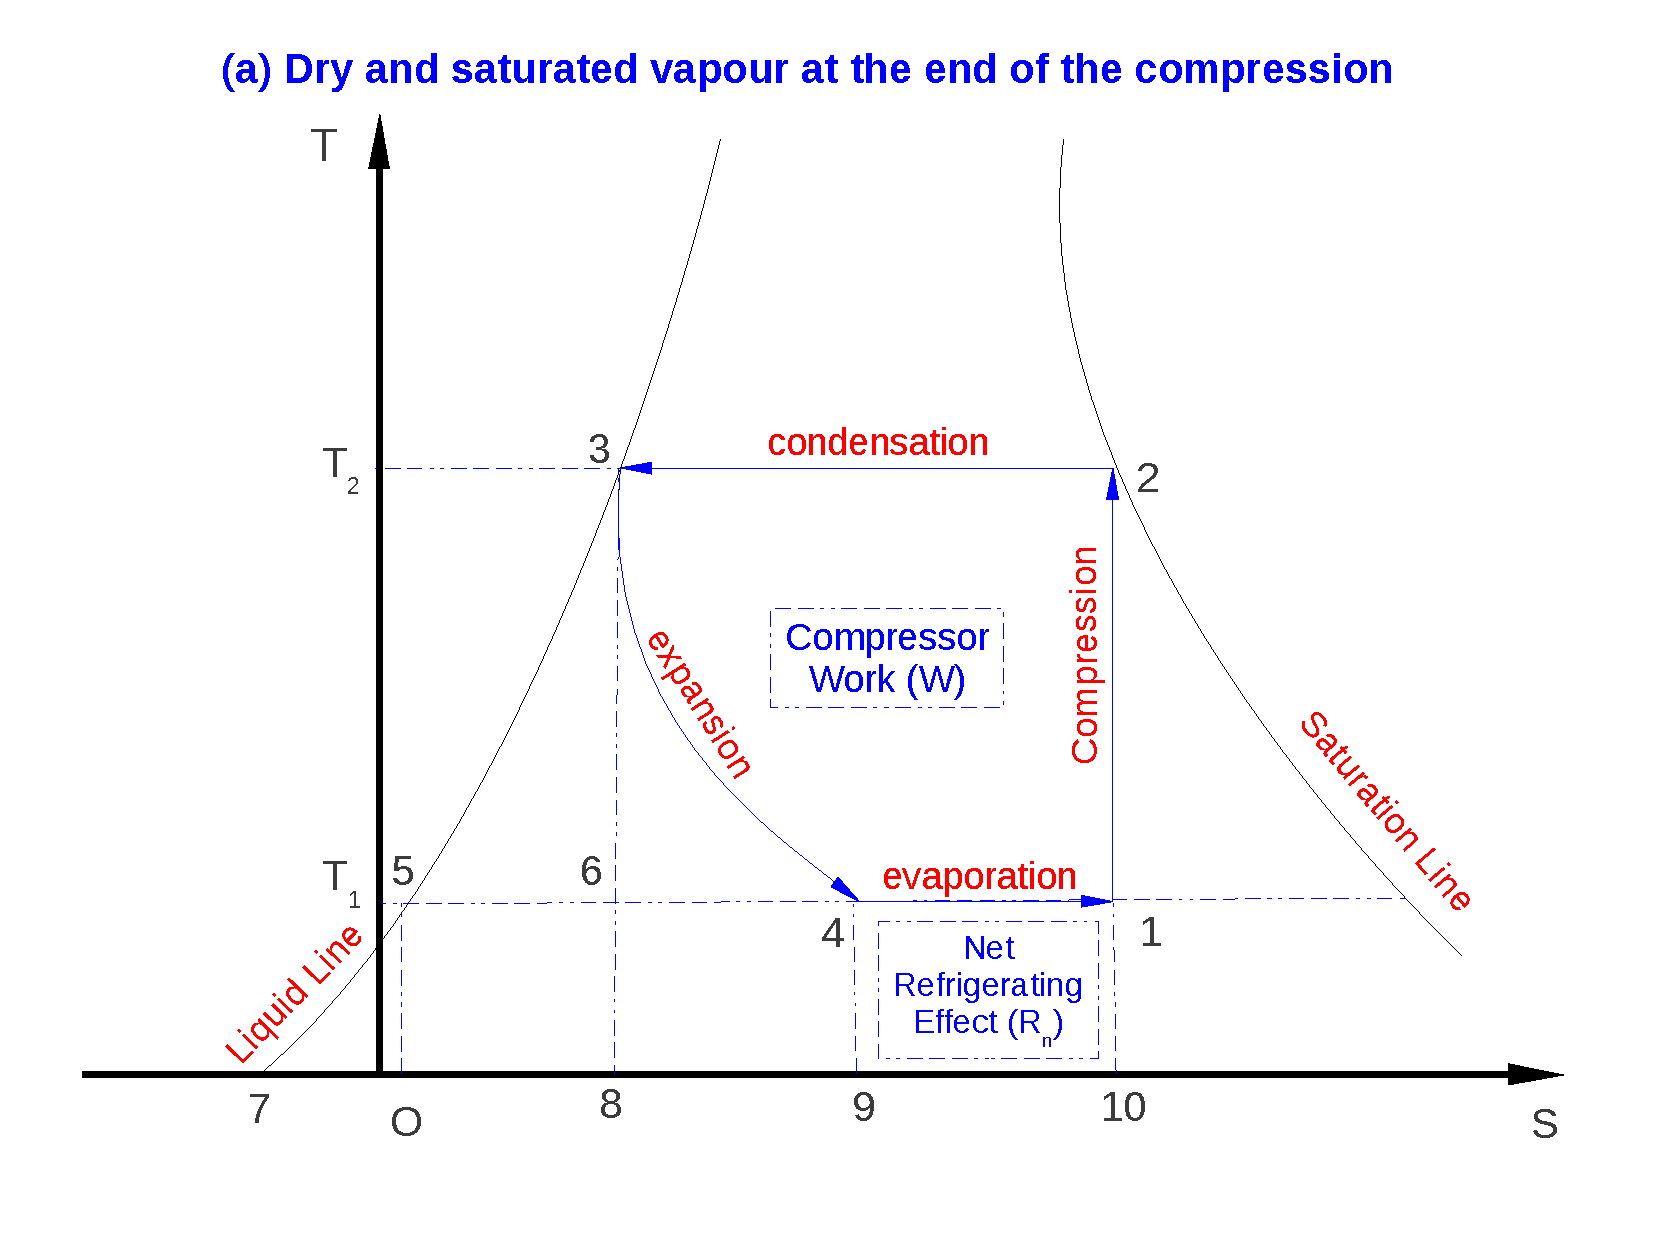
\includegraphics[width=4.cm,height=2.4cm,clip]{./Pics/Overview_Refrig14}
      \vspace{-.1cm}
      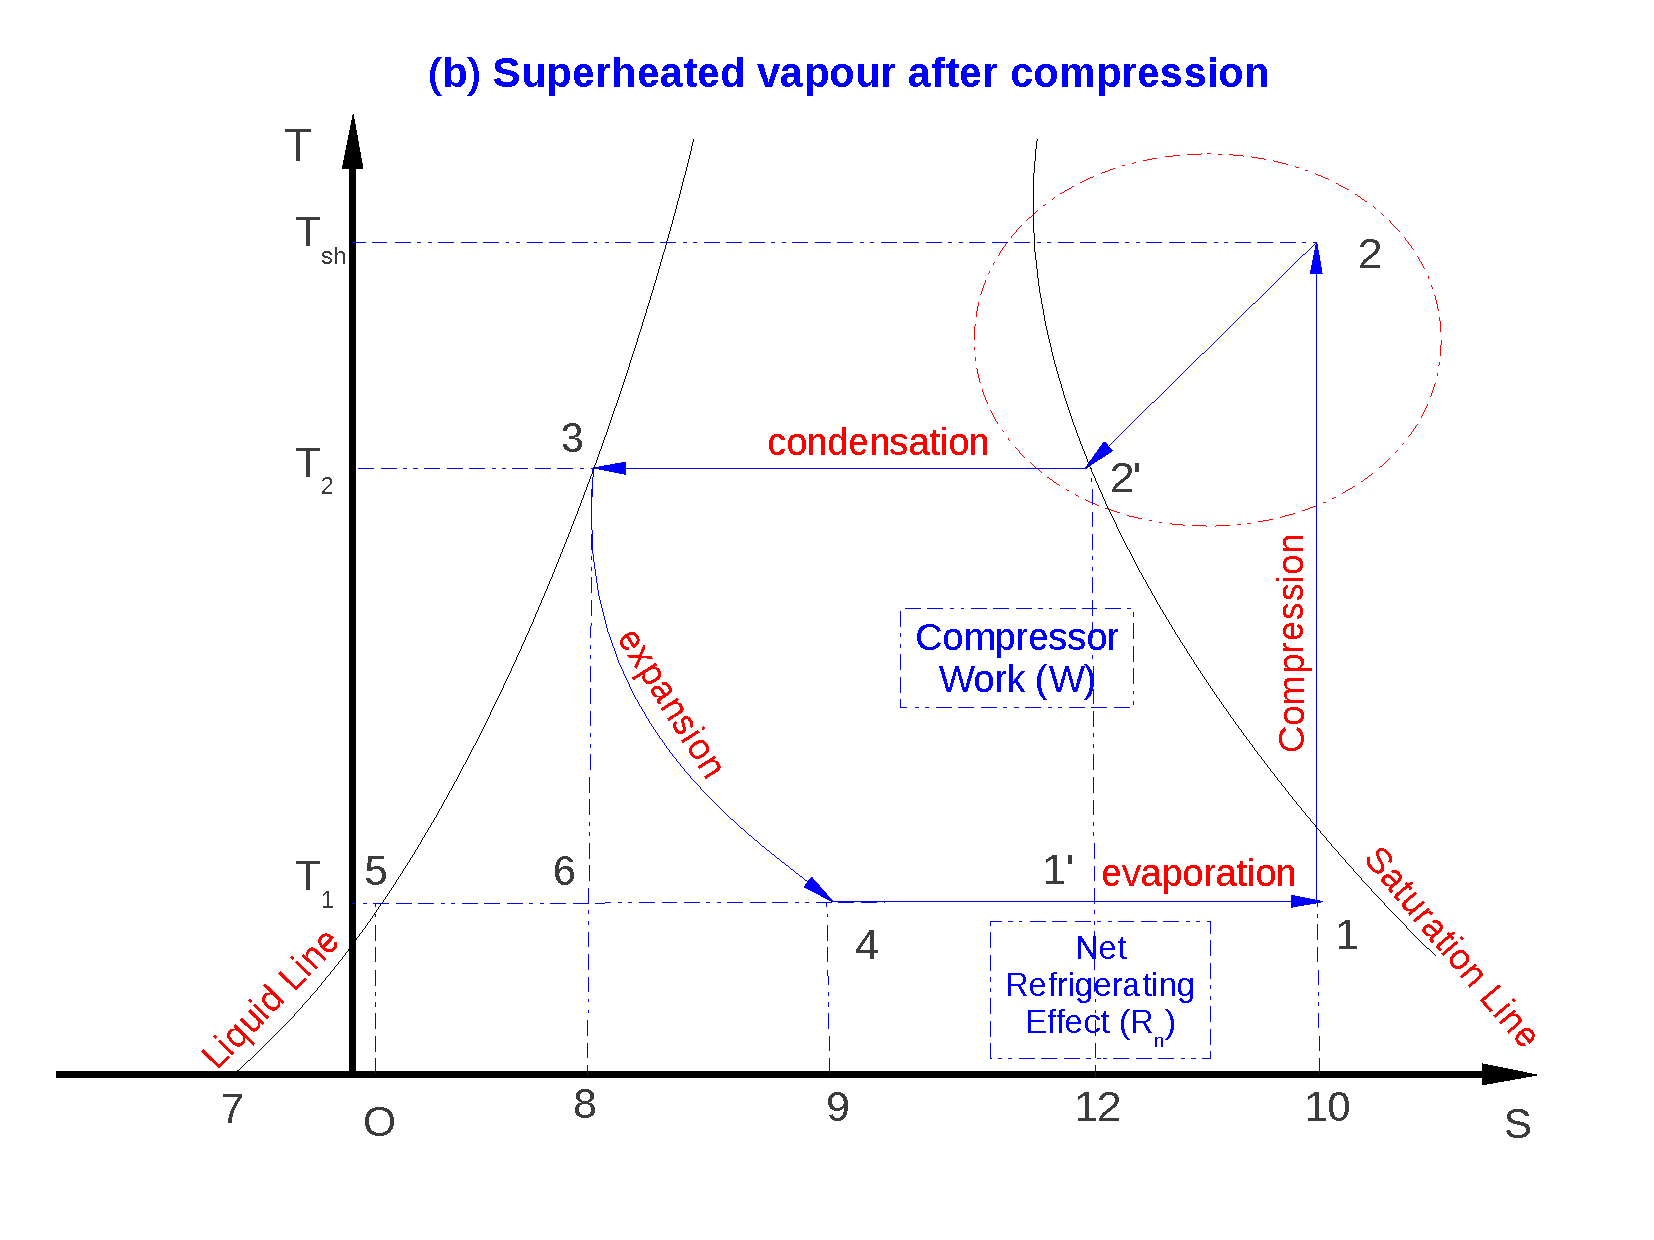
\includegraphics[width=4.cm,height=2.4cm,clip]{./Pics/Overview_Refrig15}
      \vspace{-.1cm}
      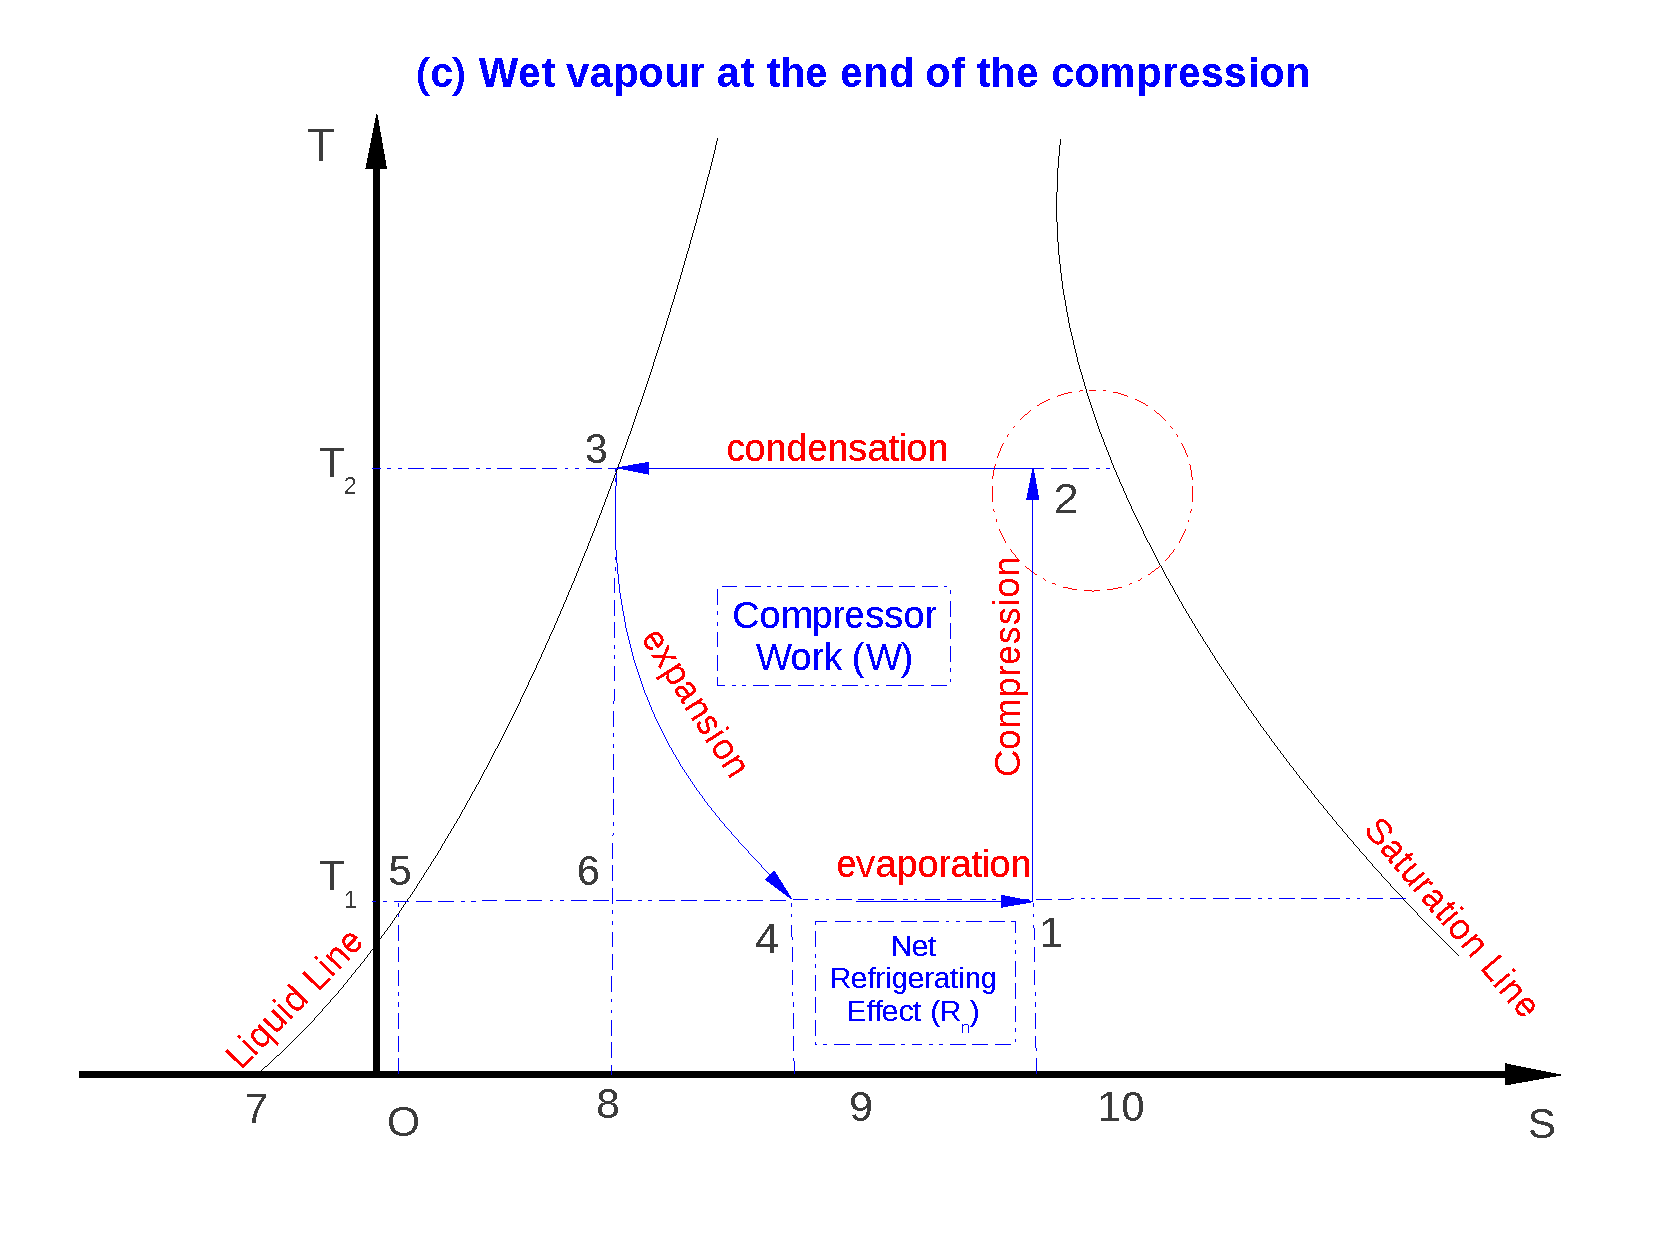
\includegraphics[width=4.cm,height=2.4cm,clip]{./Pics/Overview_Refrig16}}
   \end{figure}  
  \end{column}  
  \begin{column}[c]{0.45\linewidth}
   \begin{enumerate}[(a)]
    \item <1-> All processes of the refrigeration cycle are internally \textcolor{blue}{reversible}, \textcolor{blue}{except}; 
    \item <2-> The processes in the expansion valve which operate \textcolor{blue}{adiabatically};
    \item <3-> Refrigerant fluid that leaves the \textcolor{blue}{condenser} is \textcolor{blue}{saturated liquid}, whereas the fluid heading to the low pressure \textcolor{red}{compressor} is \textcolor{red}{saturated vapour}.
   \end{enumerate}
  \end{column}  
 \end{columns}
\end{frame}



%%%
%%% Slide
%%%
\begin{frame}
 \frametitle{Thermal Analysis -- $PH$ Diagram}
   \begin{figure}%
     \vbox{
      \hbox{\hspace{.8cm}
      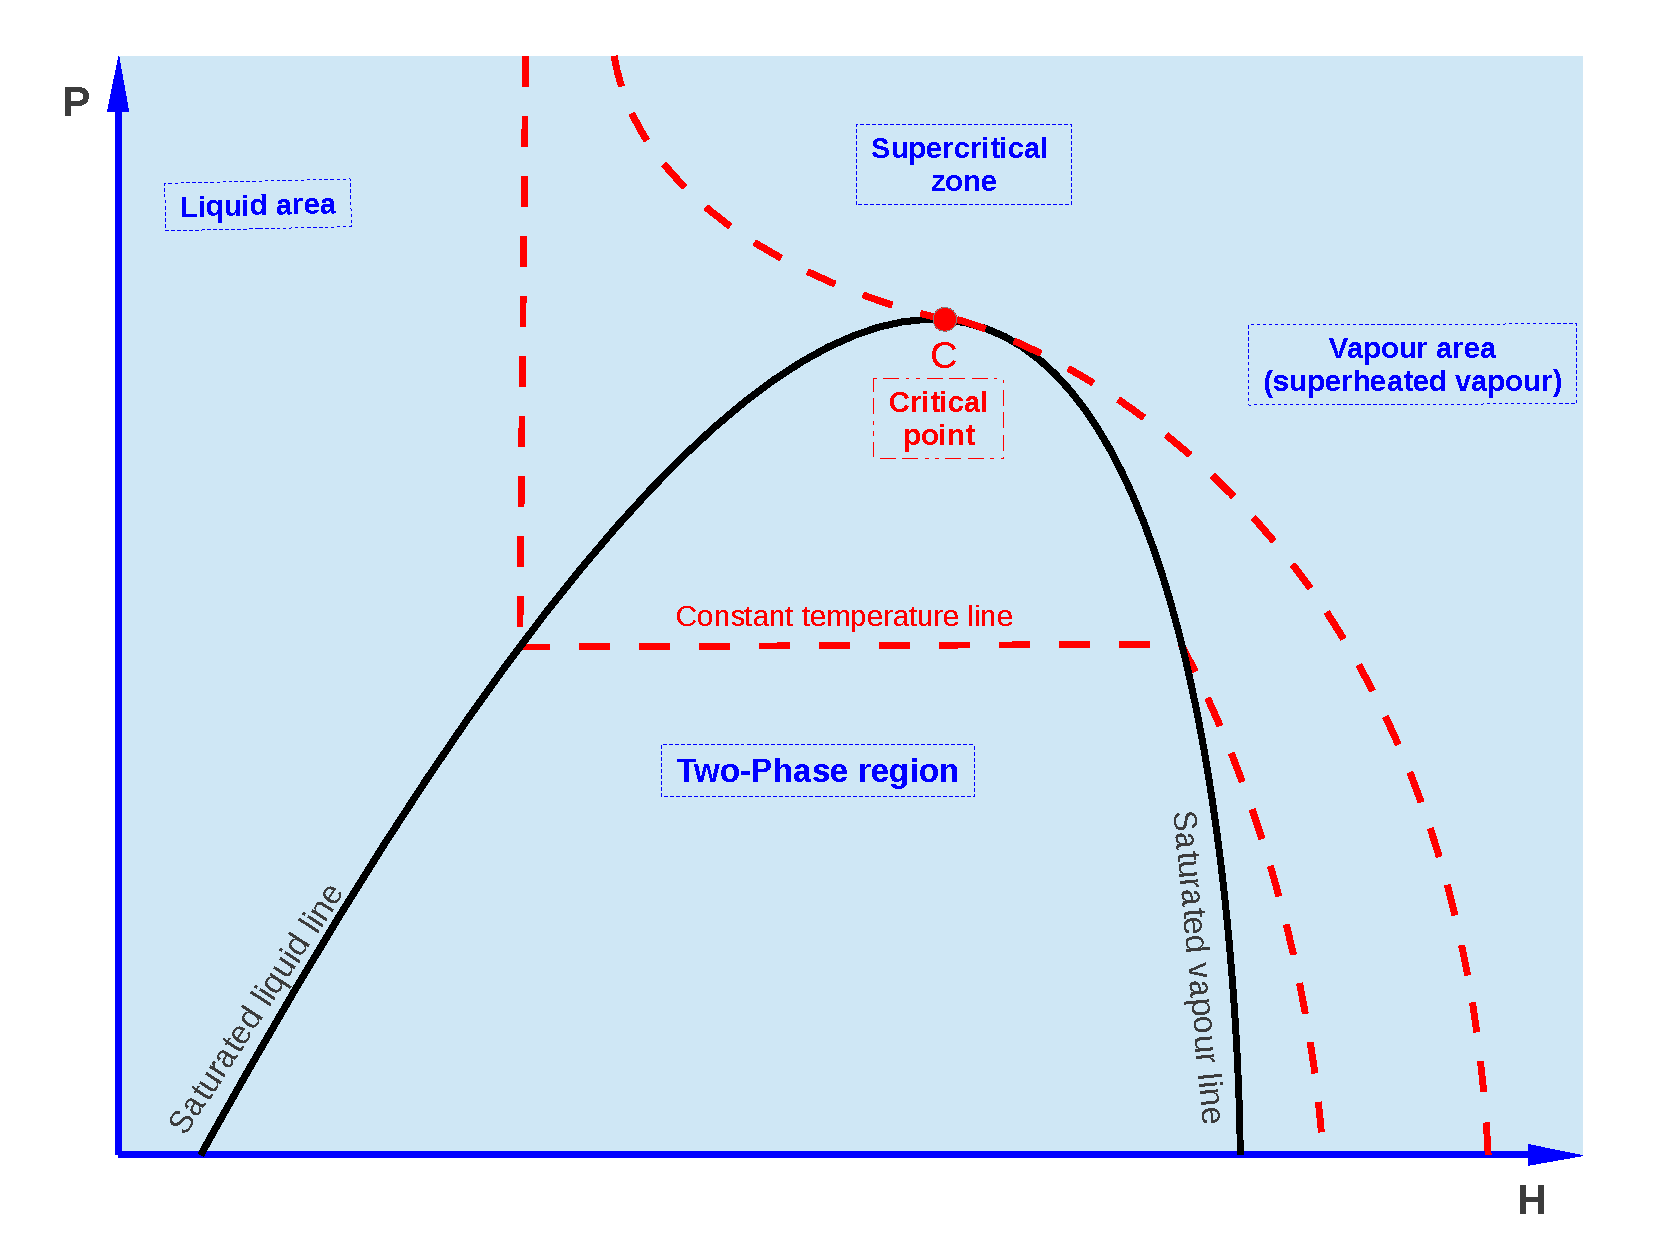
\includegraphics[width=4.6cm,height=3.8cm,clip]{./Pics/Overview_Refrig18}
      \hspace{.1cm}
      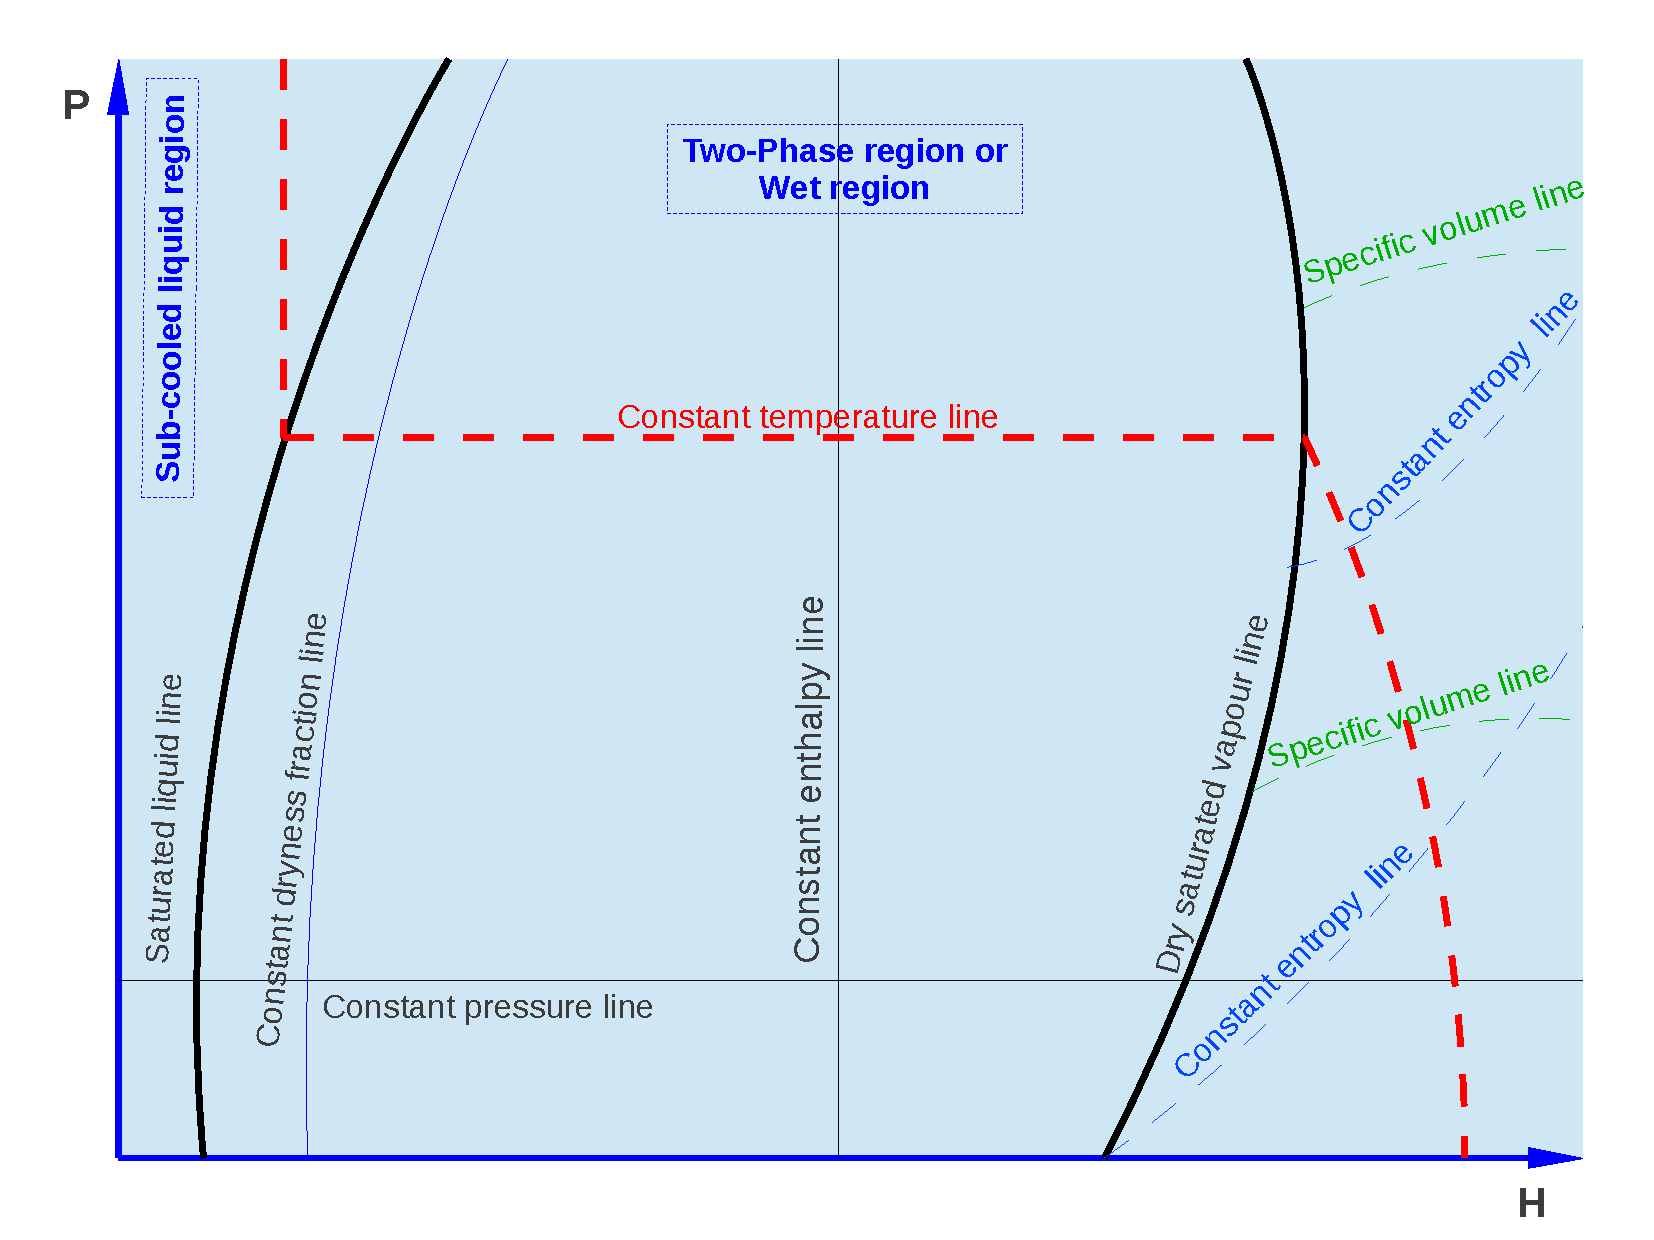
\includegraphics[width=4.6cm,height=3.8cm,clip]{./Pics/Overview_Refrig17}}
      \vspace{-.1cm}
      \hbox{\hspace{.8cm}
      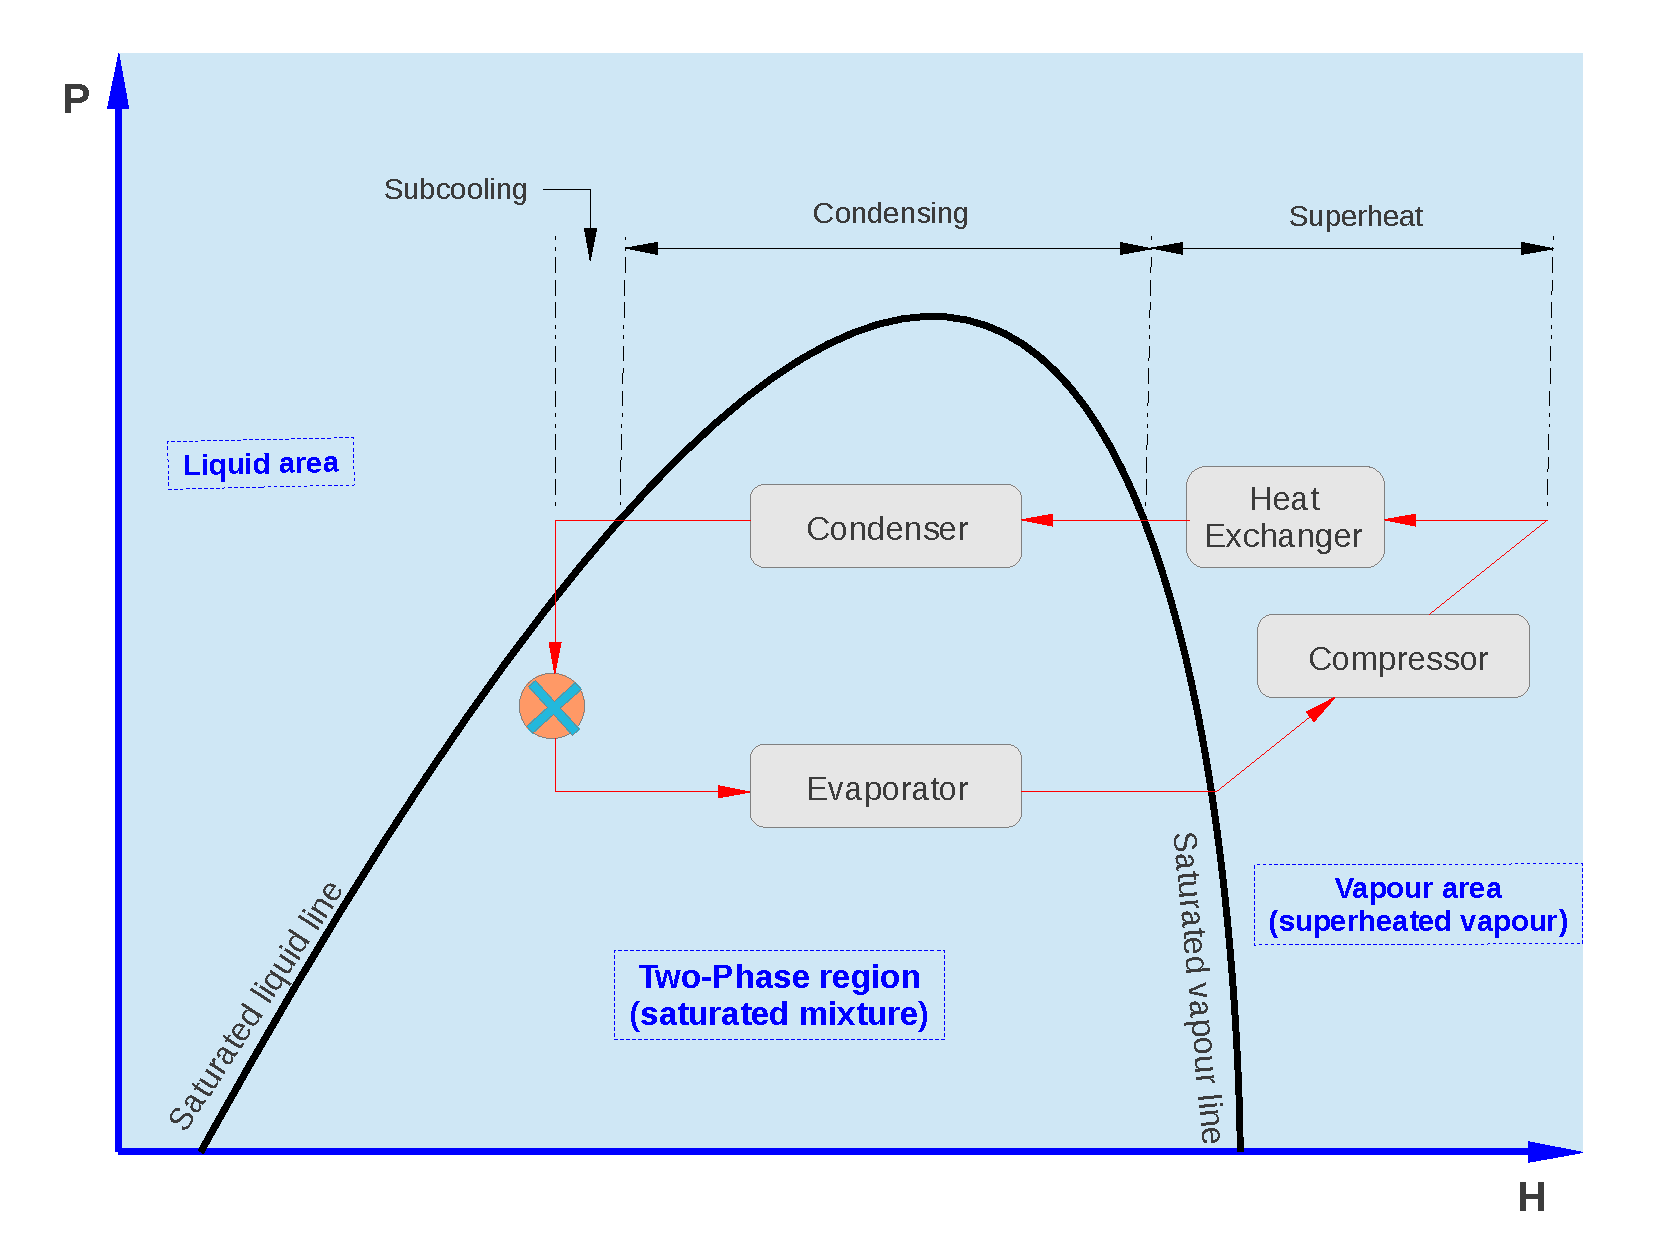
\includegraphics[width=4.6cm,height=3.87cm,clip]{./Pics/Overview_Refrig19}
      \hspace{.1cm}
      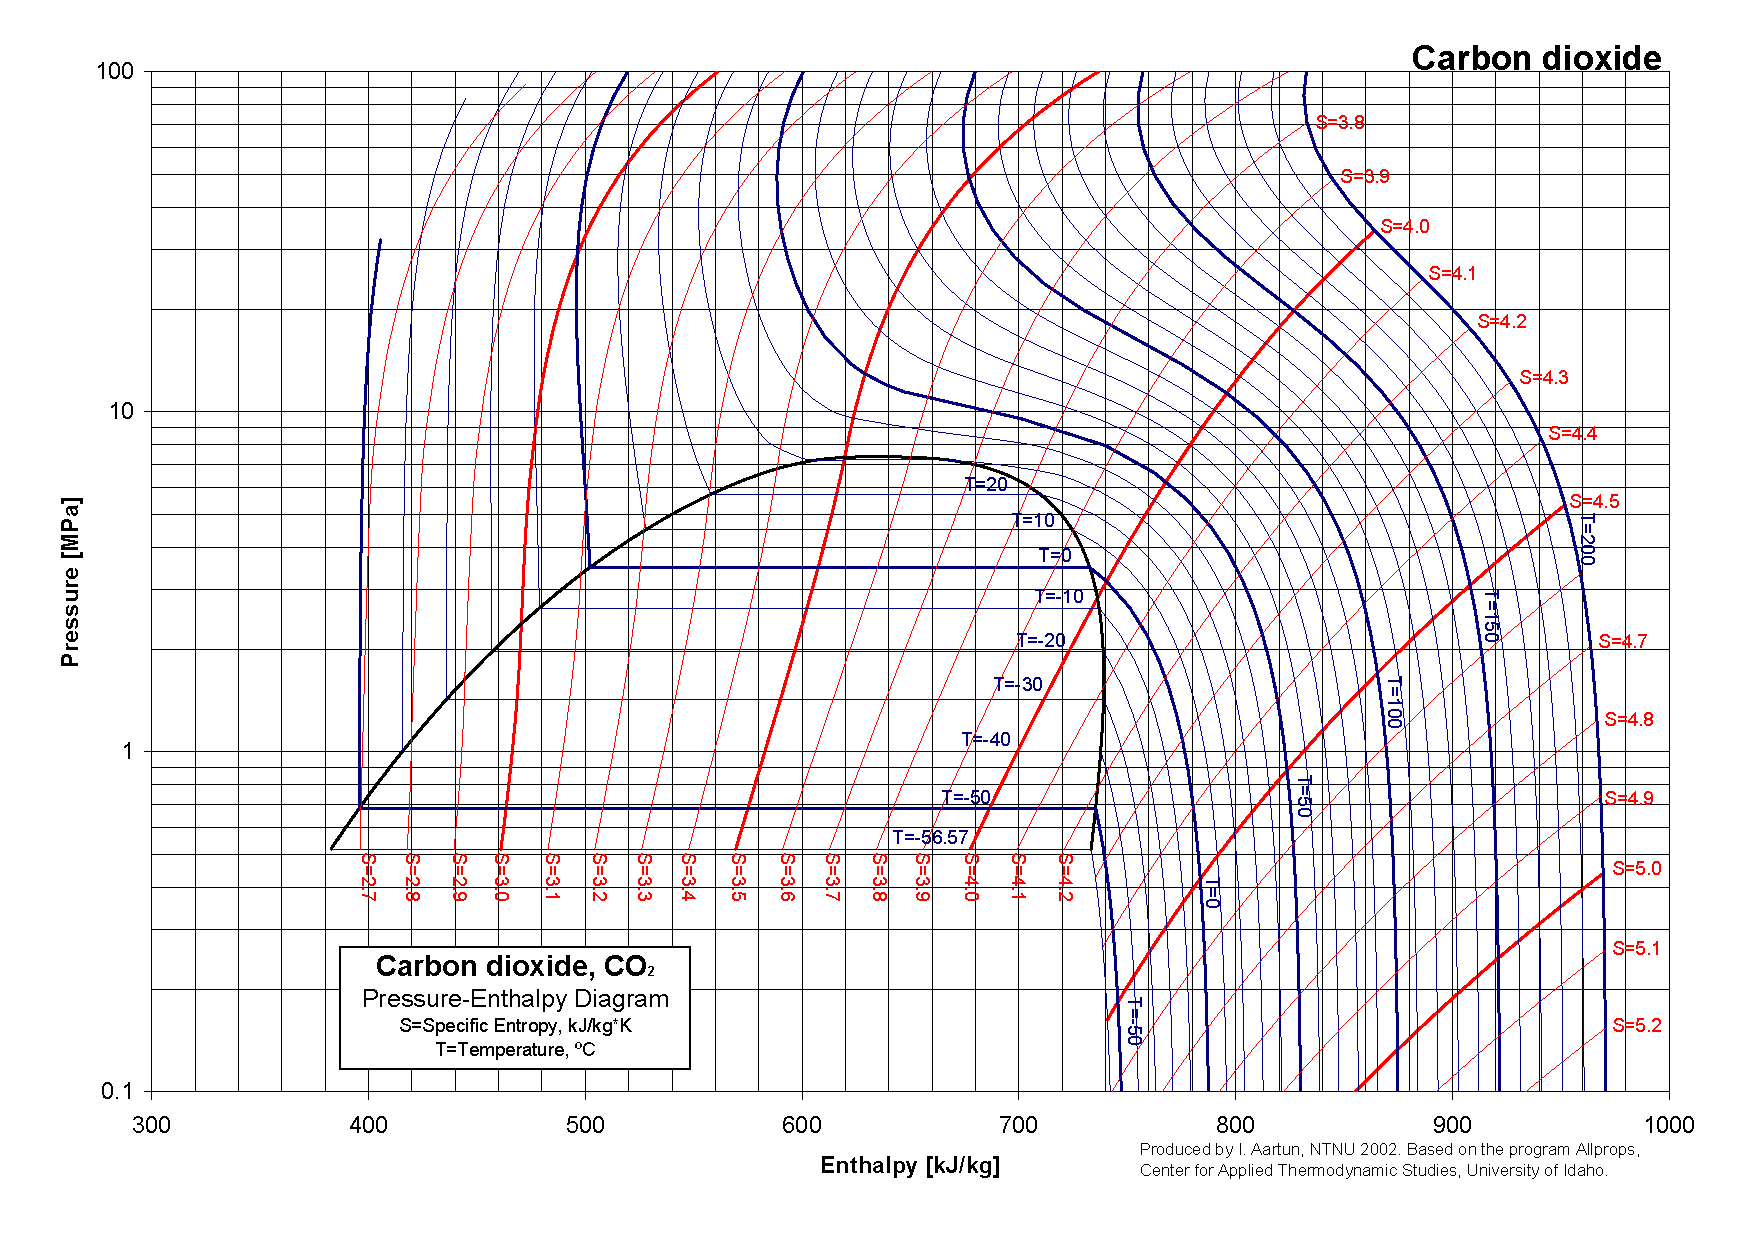
\includegraphics[width=4.9cm,height=4.cm,clip]{./Pics/CO2col}}}
   \end{figure}
\end{frame}


%%%
%%% Slide
%%%
\begin{frame}
 \frametitle{Thermal Analysis: Parameters that Affect the Performance}
 \begin{columns}
  \begin{column}[c]{0.3\linewidth}
   \begin{figure}%
      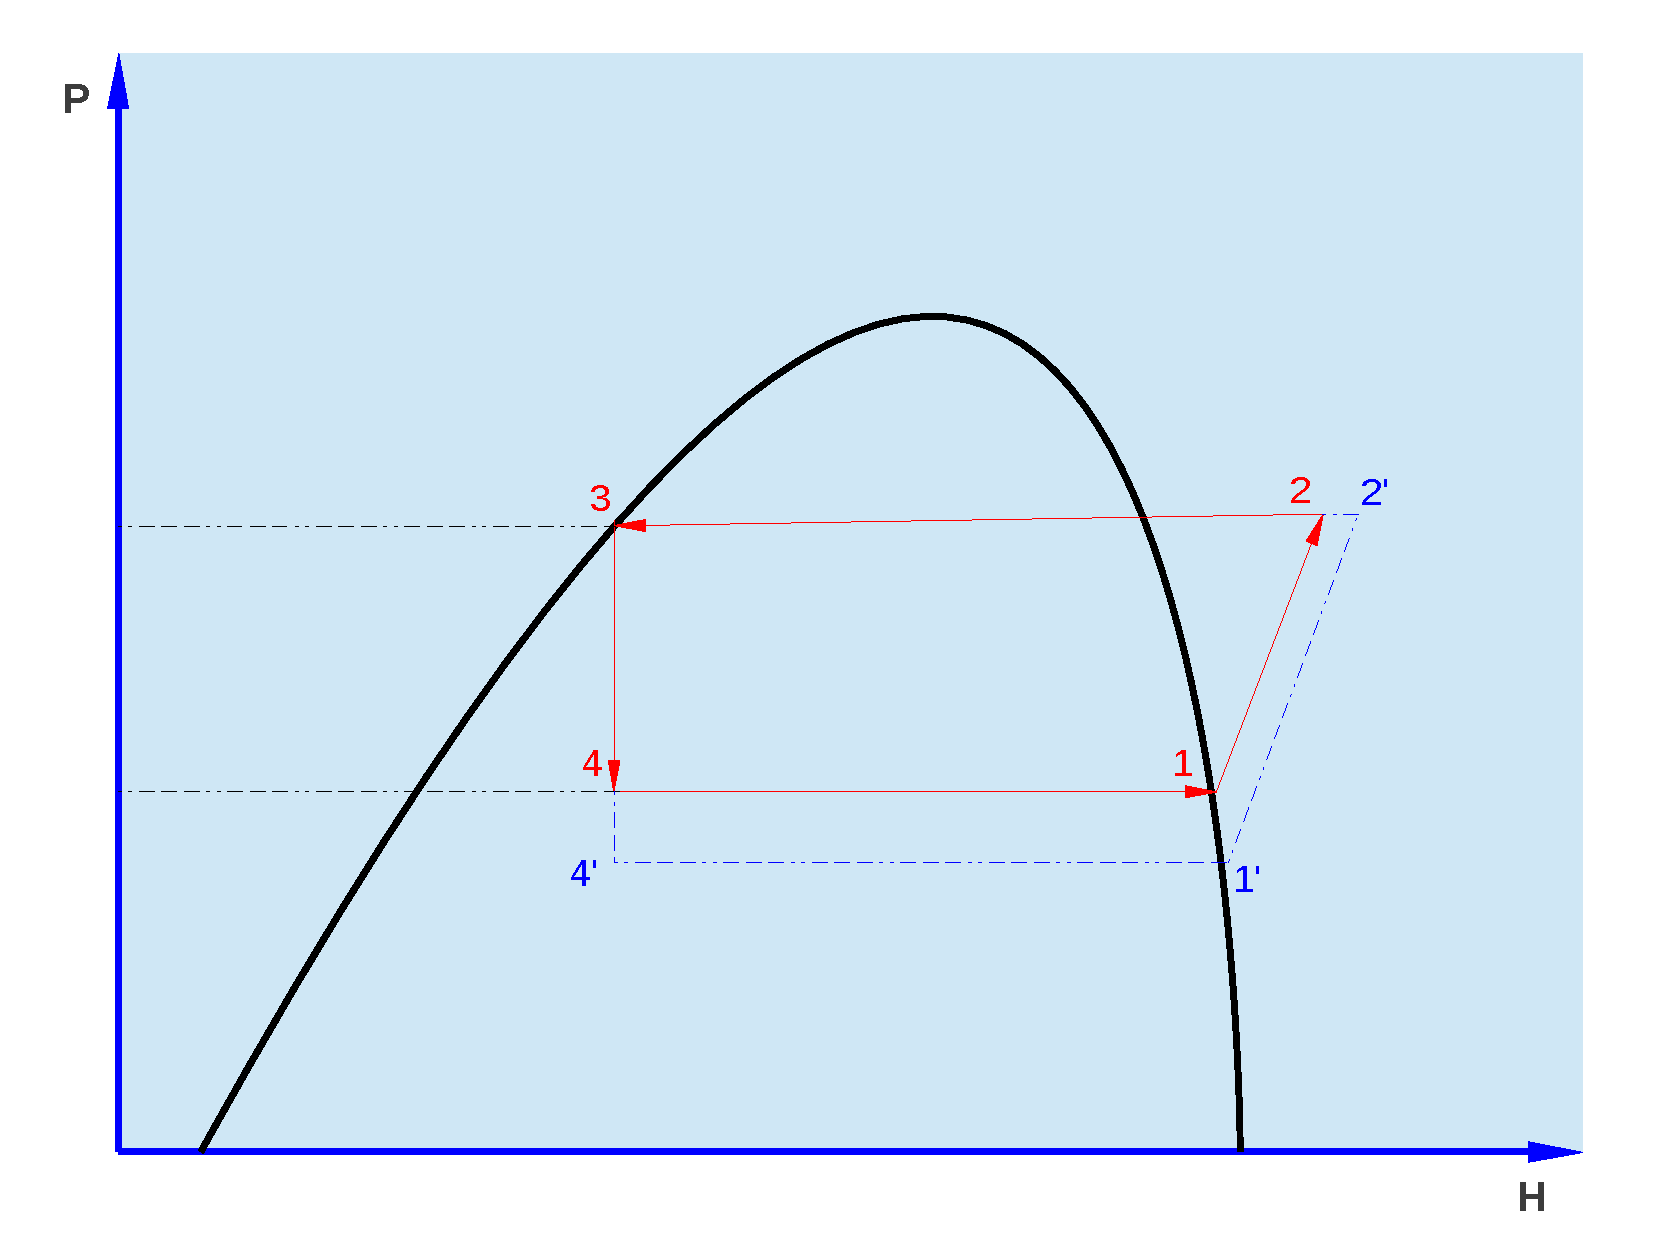
\includegraphics[width=4.cm,height=4.cm,clip]{./Pics/Overview_Refrig20}
   \end{figure}  
  \end{column}  
  \begin{column}[c]{0.7\linewidth}
   \begin{itemize}
    \item <1-> Decrease in the \textcolor{blue}{Suction Pressure} results in the following change in the COPS:
     \begin{displaymath}
       \text{COP} = \frc{R_{n}}{W}=\frc{H_{1}-H_{4}}{H_{2}-H_{1}}\;\;\;\text{original cycle;}
     \end{displaymath}
     \begin{eqnarray}
      \text{COP}&=&\frc{H_{1'}-H_{4'}}{H_{2'}-H_{1'}}\;\;\text{with } H_{4}=H_{4'} \nonumber \\
                                  &=& \frc{\left(H_{1}-H_{4}\right)-\left(H_{1}-H_{1'}\right)}{\left(H_{2}-H_{1}\right)+\left(H_{1}-H_{1'}\right)+\left(H_{2'}-H_{2}\right)} \nonumber 
     \end{eqnarray} 
    \item <2-> The above expression show that the refrigerating effect decreases whereas the work increases with the decrease of the suction pressure in the expansion valve output.
   \end{itemize}
  \end{column}  
 \end{columns}
\end{frame}



%%%
%%% Slide
%%%
\begin{frame}
 \frametitle{Thermal Analysis: Parameters that Affect the Performance}
 \begin{columns}
  \begin{column}[c]{0.3\linewidth}
   \begin{figure}%
      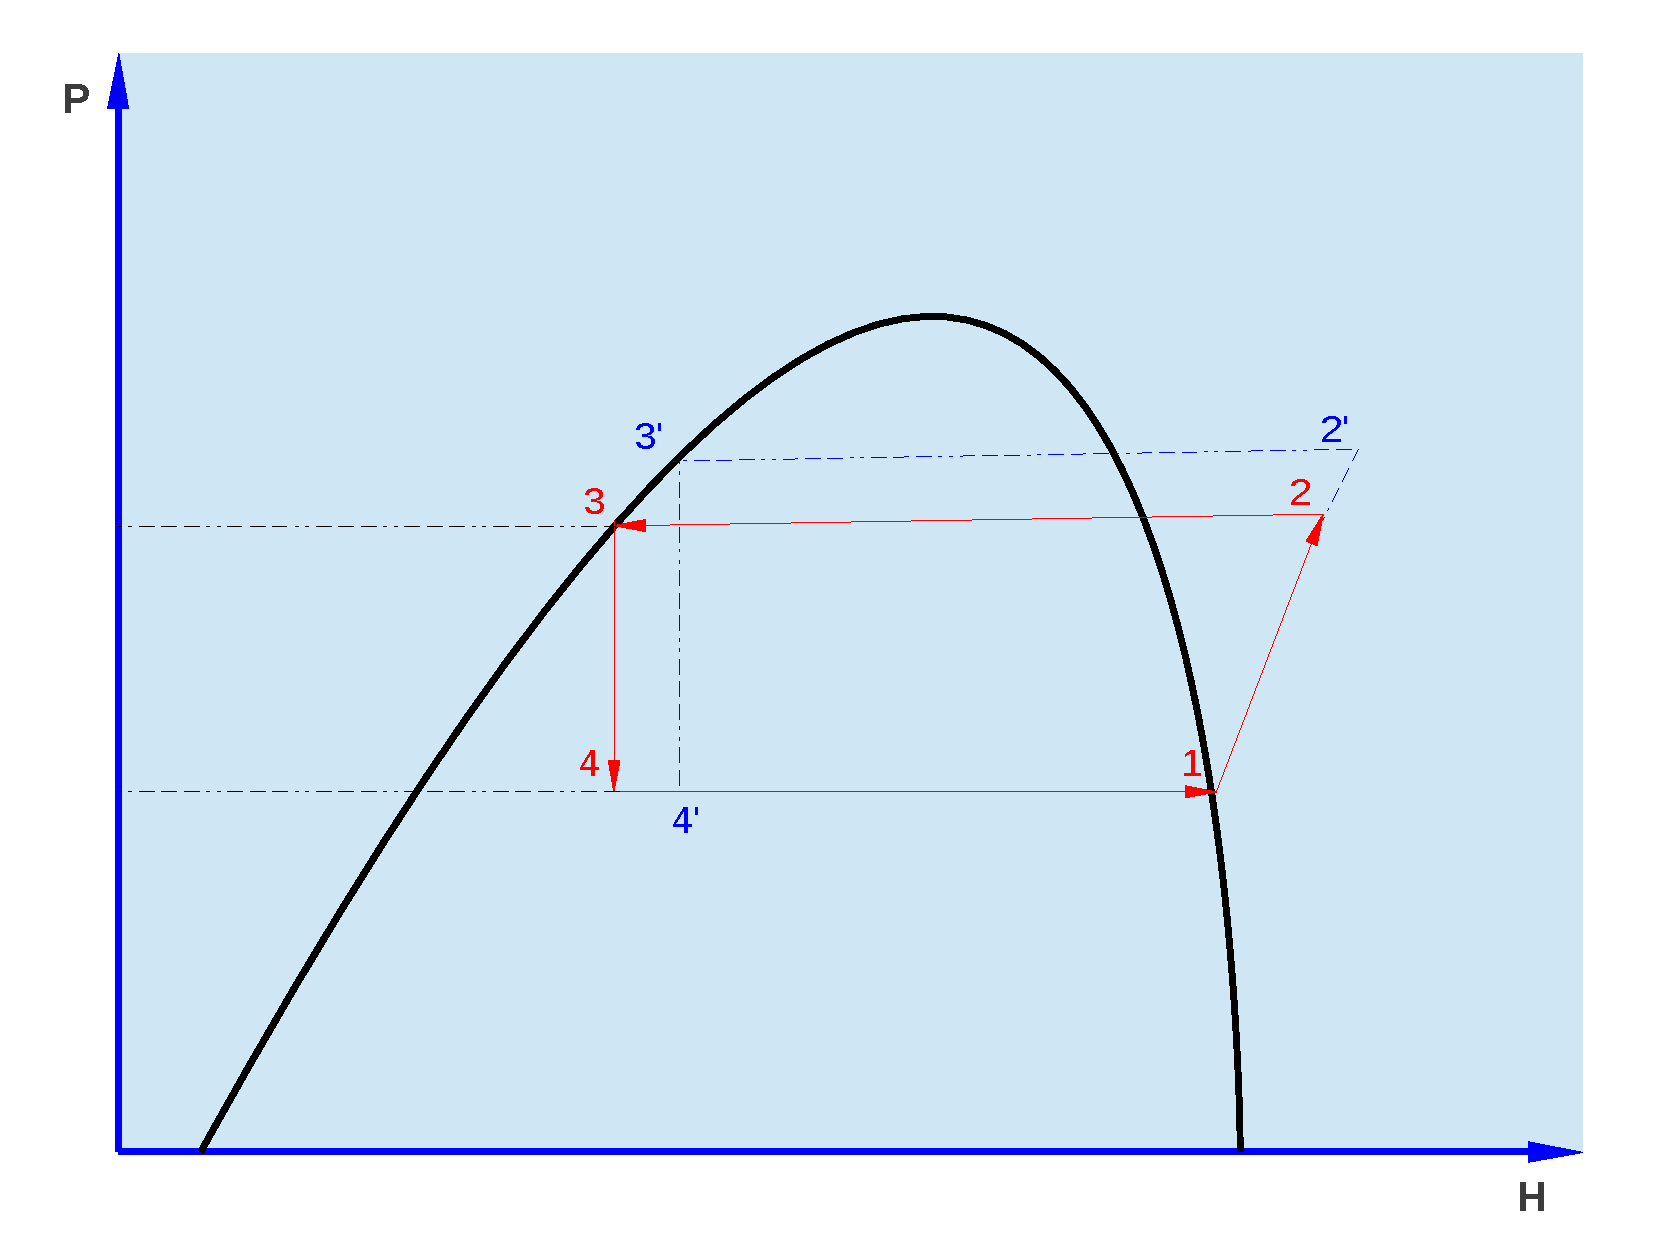
\includegraphics[width=4.cm,height=4.cm,clip]{./Pics/Overview_Refrig21}
   \end{figure}  
  \end{column}  
  \begin{column}[c]{0.7\linewidth}
   \begin{itemize}
    \item <1-> Increase in the \textcolor{blue}{Discharge Pressure} (in the entrance of the expansion valve) results in the following change in the COPS:
     \begin{eqnarray}
      \text{COP}&=&\frc{H_{1}-H_{4'}}{H_{2'}-H_{1}} \nonumber \\
                                  &=& \frc{\left(H_{1}-H_{4}\right)-\left(H_{4'}-H_{4}\right)}{\left(H_{2}-H_{1}\right)+\left(H_{2'}-H_{2}\right)} \nonumber 
     \end{eqnarray} 
    \item <2-> The  effect of increasing the discharge pressure is similar to the effect of suction pressure.
   \end{itemize}
  \end{column}  
 \end{columns}
\end{frame}


%%%
%%% Slide
%%%
\begin{frame}
 \frametitle{Thermal Analysis: Parameters that Affect the Performance}
 \begin{columns}
  \begin{column}[c]{0.3\linewidth}
   \begin{figure}%
      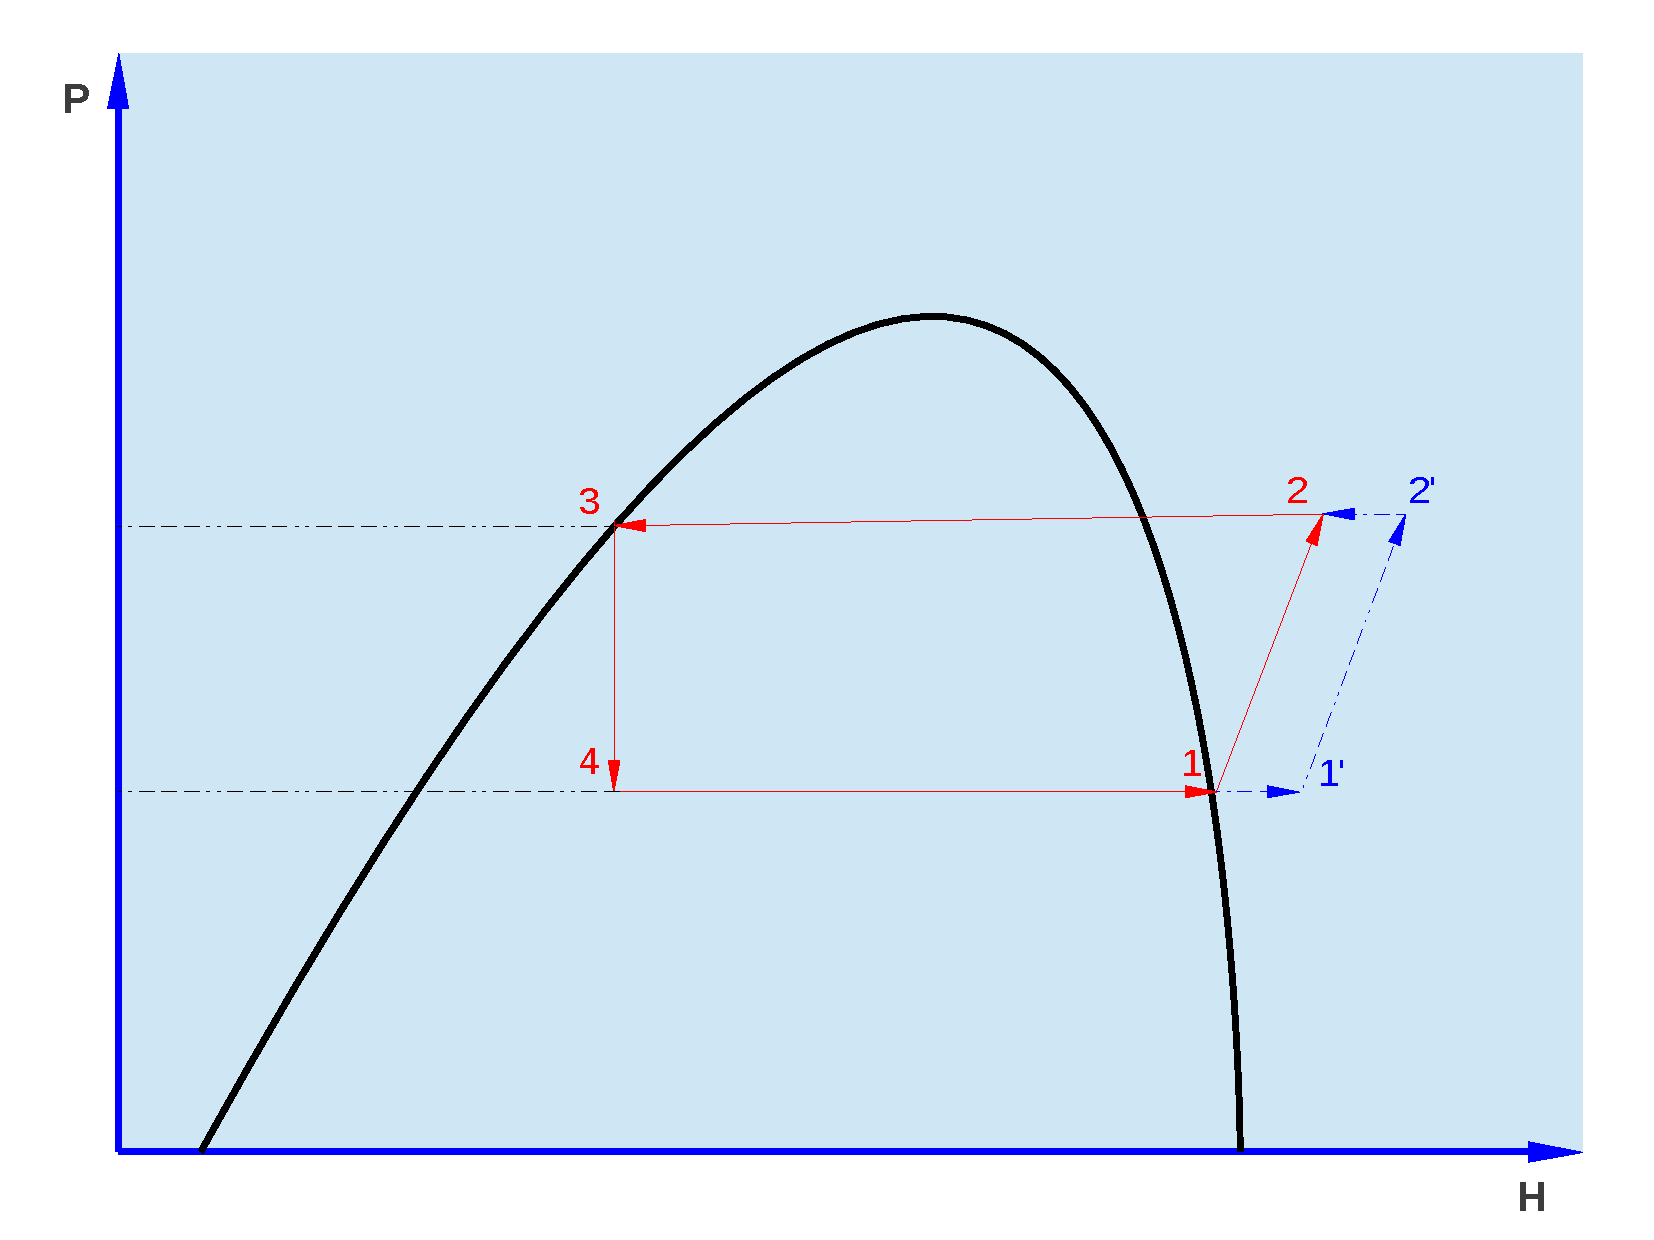
\includegraphics[width=4.cm,height=4.cm,clip]{./Pics/Overview_Refrig22}
   \end{figure}  
  \end{column}  
  \begin{column}[c]{0.7\linewidth}
   \begin{itemize}
    \item <1-> Increasing the \textcolor{blue}{superheated effect} leads to the increase of the refrigerating effect with a substantial increase of the amount of work spent to keep the upper pressure limit,
     \begin{eqnarray}
      \text{COP}&=&\frc{H_{1'}-H_{4}}{H_{2'}-H_{1'}} \nonumber \\
                                  &=& \frc{\left(H_{1}-H_{4}\right)-\left(H_{1}-H_{1'}\right)}{\left(H_{2}-H_{1}\right)+\left(H_{2'}-H_{2}\right)+\left(H_{1}-H_{1'}\right)} \nonumber 
     \end{eqnarray} 
    \item <2-> Usually the increase in work is larger than the increase in the refrigerating effect, leading to a lower COP.
   \end{itemize}
  \end{column}  
 \end{columns}
\end{frame}


%%%
%%% Slide
%%%
\begin{frame}
 \frametitle{Thermal Analysis: Parameters that Affect the Performance}
 \begin{columns}
  \begin{column}[c]{0.3\linewidth}
   \begin{figure}%
      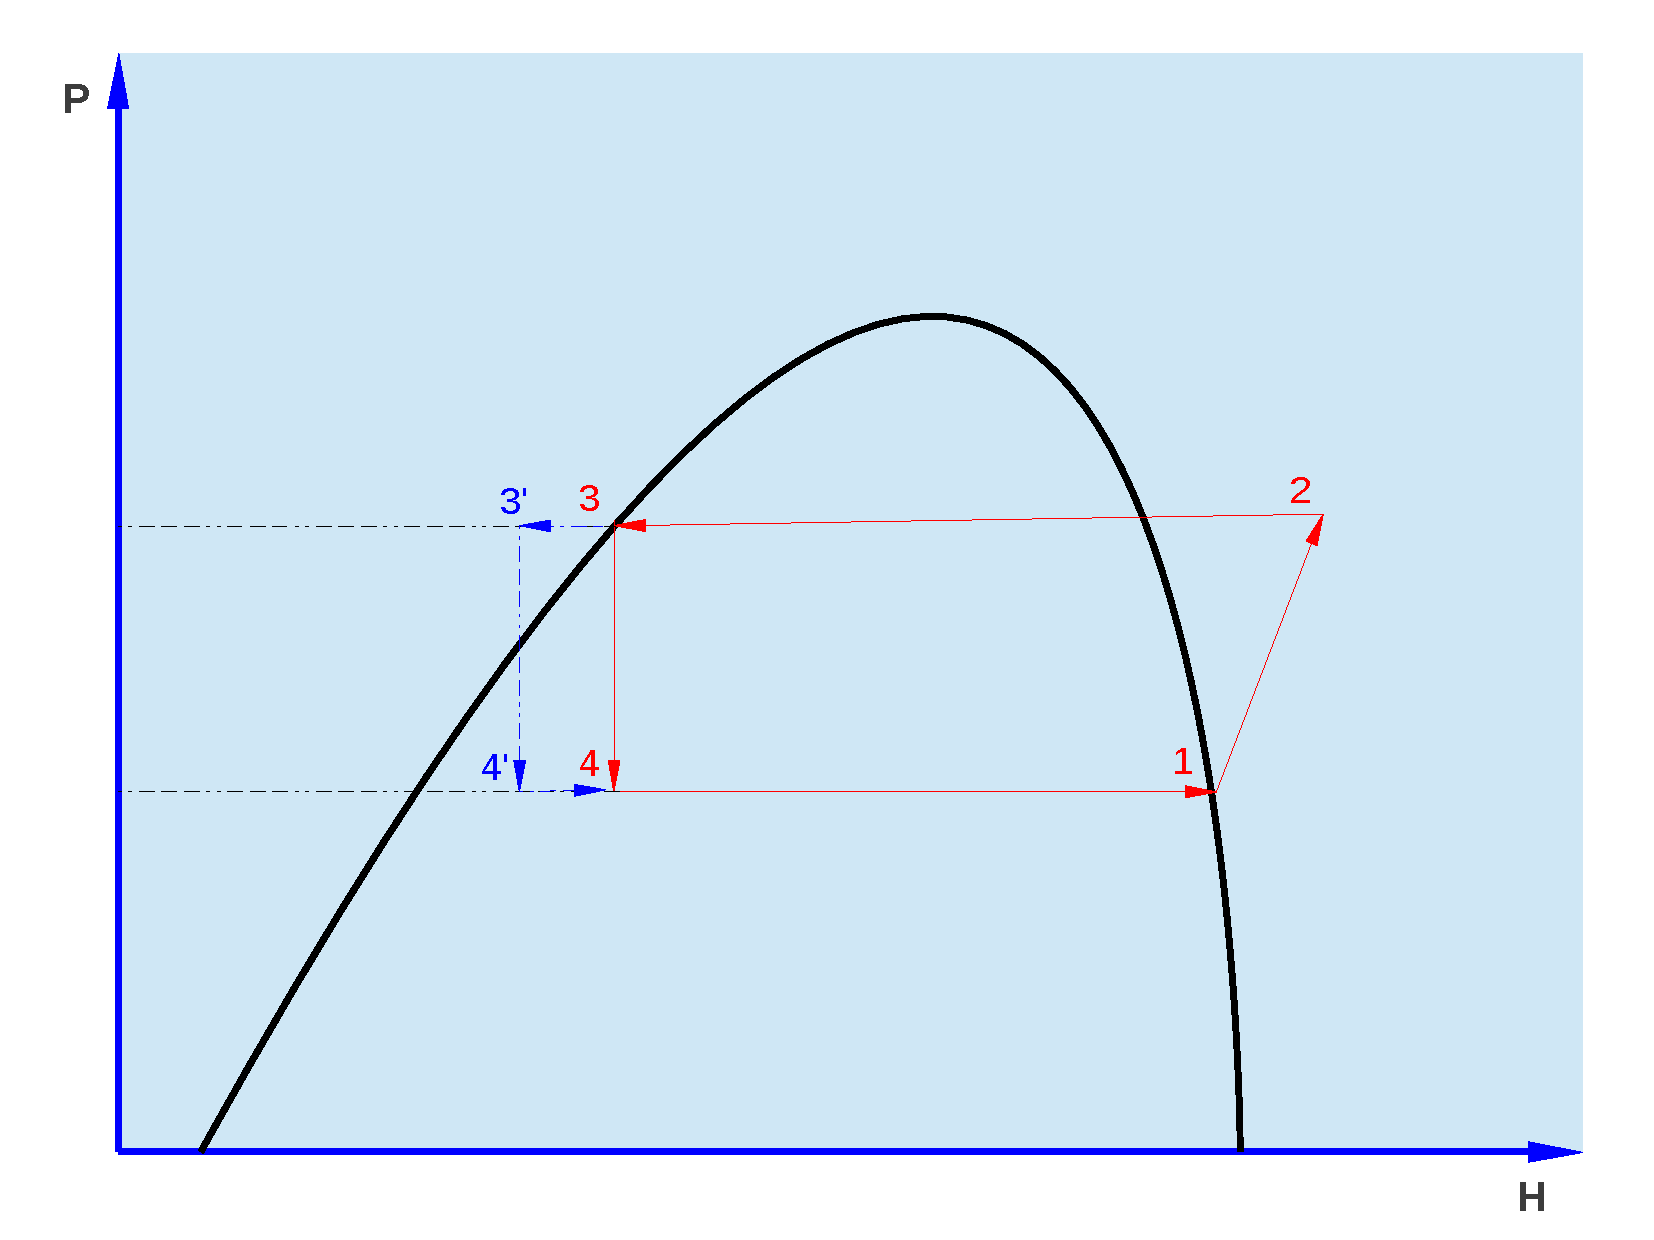
\includegraphics[width=4.cm,height=4.cm,clip]{./Pics/Overview_Refrig23}
   \end{figure}  
  \end{column}  
  \begin{column}[c]{0.7\linewidth}
   \begin{itemize}
    \item <1-> \textcolor{blue}{Sub-cooling} is the process of cooling the fluid \textcolor{blue}{below the condensing temperature} for a given pressure.
     \begin{eqnarray}
      \text{COP}&=&\frc{H_{1}-H_{4'}}{H_{2}-H_{1}} \nonumber \\
                                  &=& \frc{\left(H_{1}-H_{4}\right)+\left(H_{4}-H_{4'}\right)}{\left(H_{2}-H_{1}\right)} \nonumber 
     \end{eqnarray} 
    \item <2-> The sub-cooling (3-3') results in the increasing of the refrigerating effect that leads to an increase of COP (provided that no further energy is spent to obtain extra cold coolant).
   \end{itemize}
  \end{column}  
 \end{columns}
\end{frame}

%%%
%%% Slide
%%%
\begin{frame}
 \frametitle{Thermal Analysis: Volumetric Efficiency of the Compressor}
 \begin{columns}
  \begin{column}[c]{0.45\linewidth}
   \begin{figure}%
      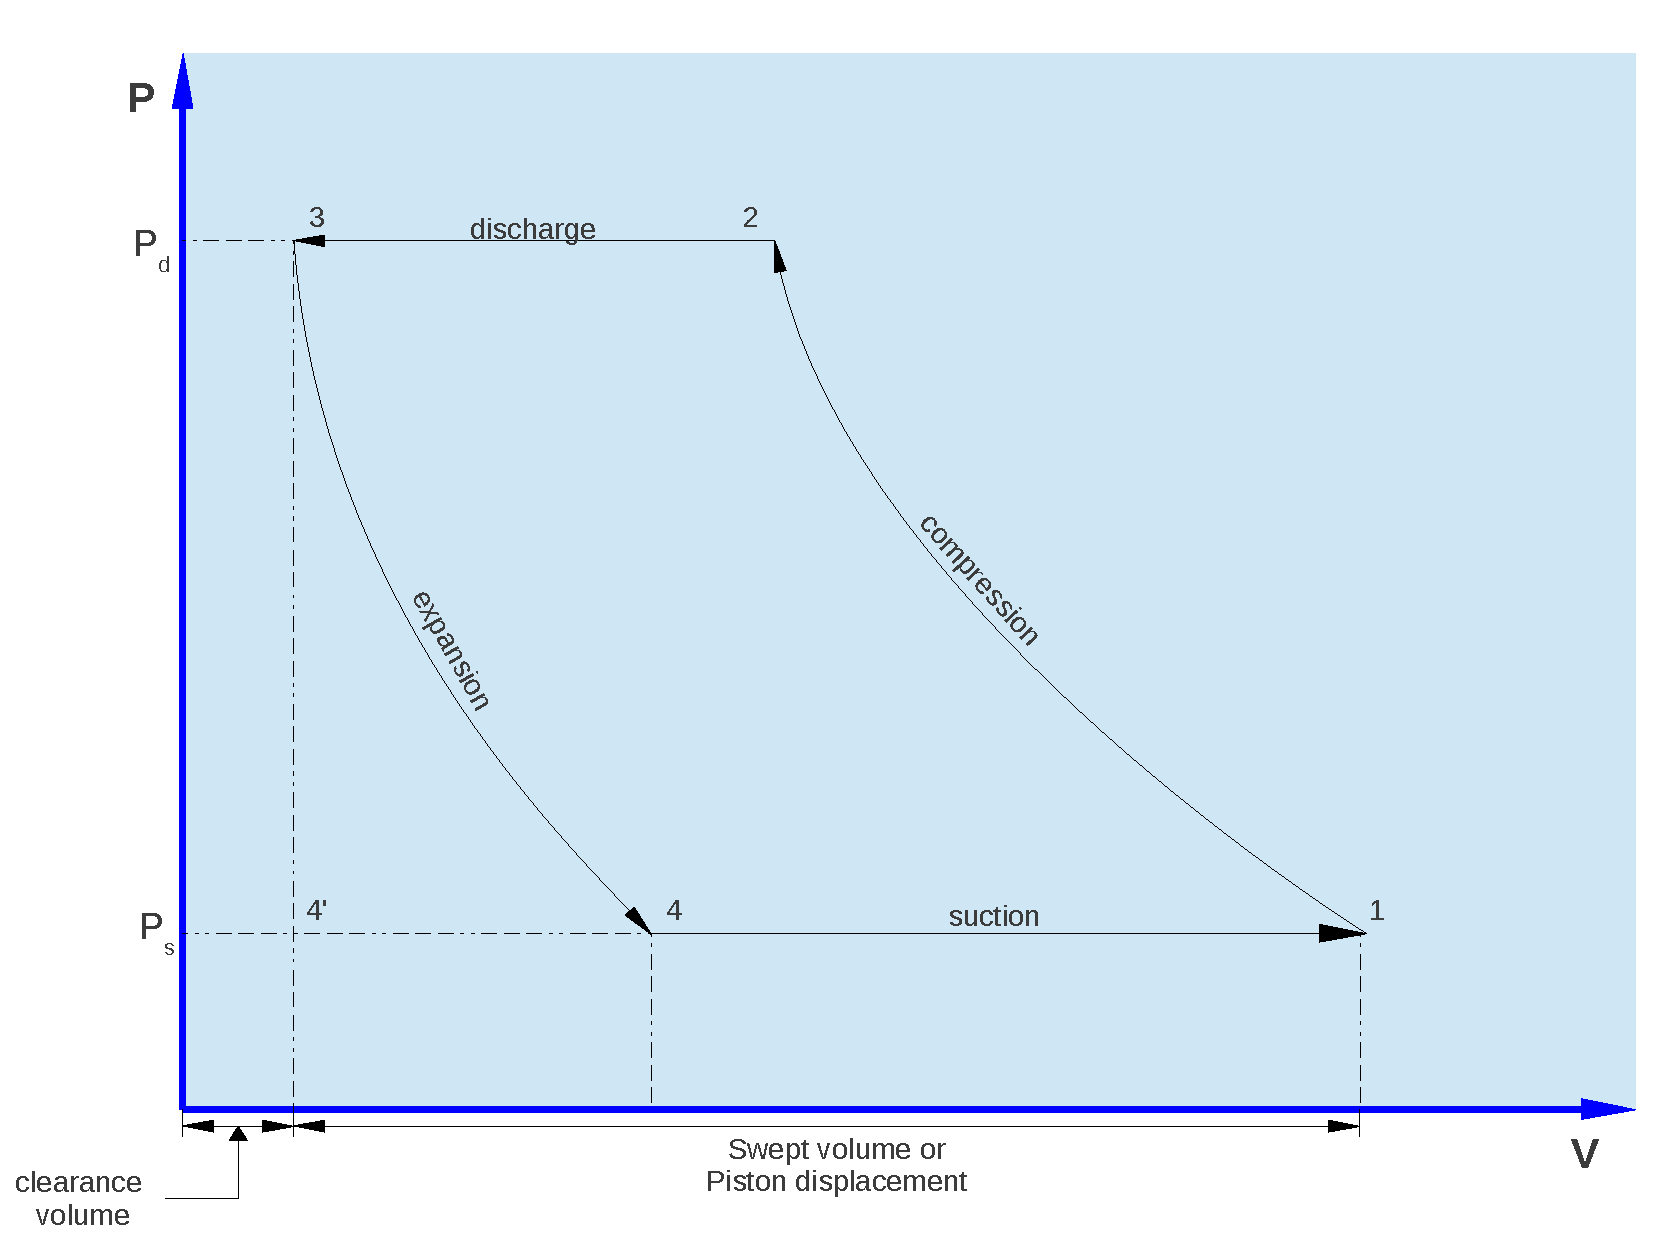
\includegraphics[width=5.cm,height=5.cm,clip]{./Pics/Overview_Refrig29}
   \end{figure}  
  \end{column}  
  \begin{column}[c]{0.55\linewidth}
   \begin{itemize}
    \item <1-> In ideal compression processes, we assume that there is neither clearance volume nor losses (e.g., friction, leakage of fluid past the piston or valves, etc);
    \item <2-> In actual compression all these mechanical and thermal losses have strong impact in the efficiency of the compressor and, therefore the refrigeration cycle;
    \item <3-> \textcolor{blue}{{\it Volumetric efficiency}} $\lq${\it is the ratio of actual volume of gas drawn into the compressor (at evaporator temperature and pressure) on each stroke to the piston displacement'};
    \item <4-> If we focus our efficiency analysis only on the influence of the {\it clearance volume} $\Rightarrow$ \textcolor{blue}{Clearance Volumetric Efficiency}.
   \end{itemize} 
  \end{column}  
 \end{columns}
\end{frame}


%%%
%%% Slide
%%%
\begin{frame}
 \frametitle{Thermal Analysis: Volumetric Efficiency of the Compressor}
 \begin{columns}
  \begin{column}[c]{0.45\linewidth}
   \begin{figure}%
      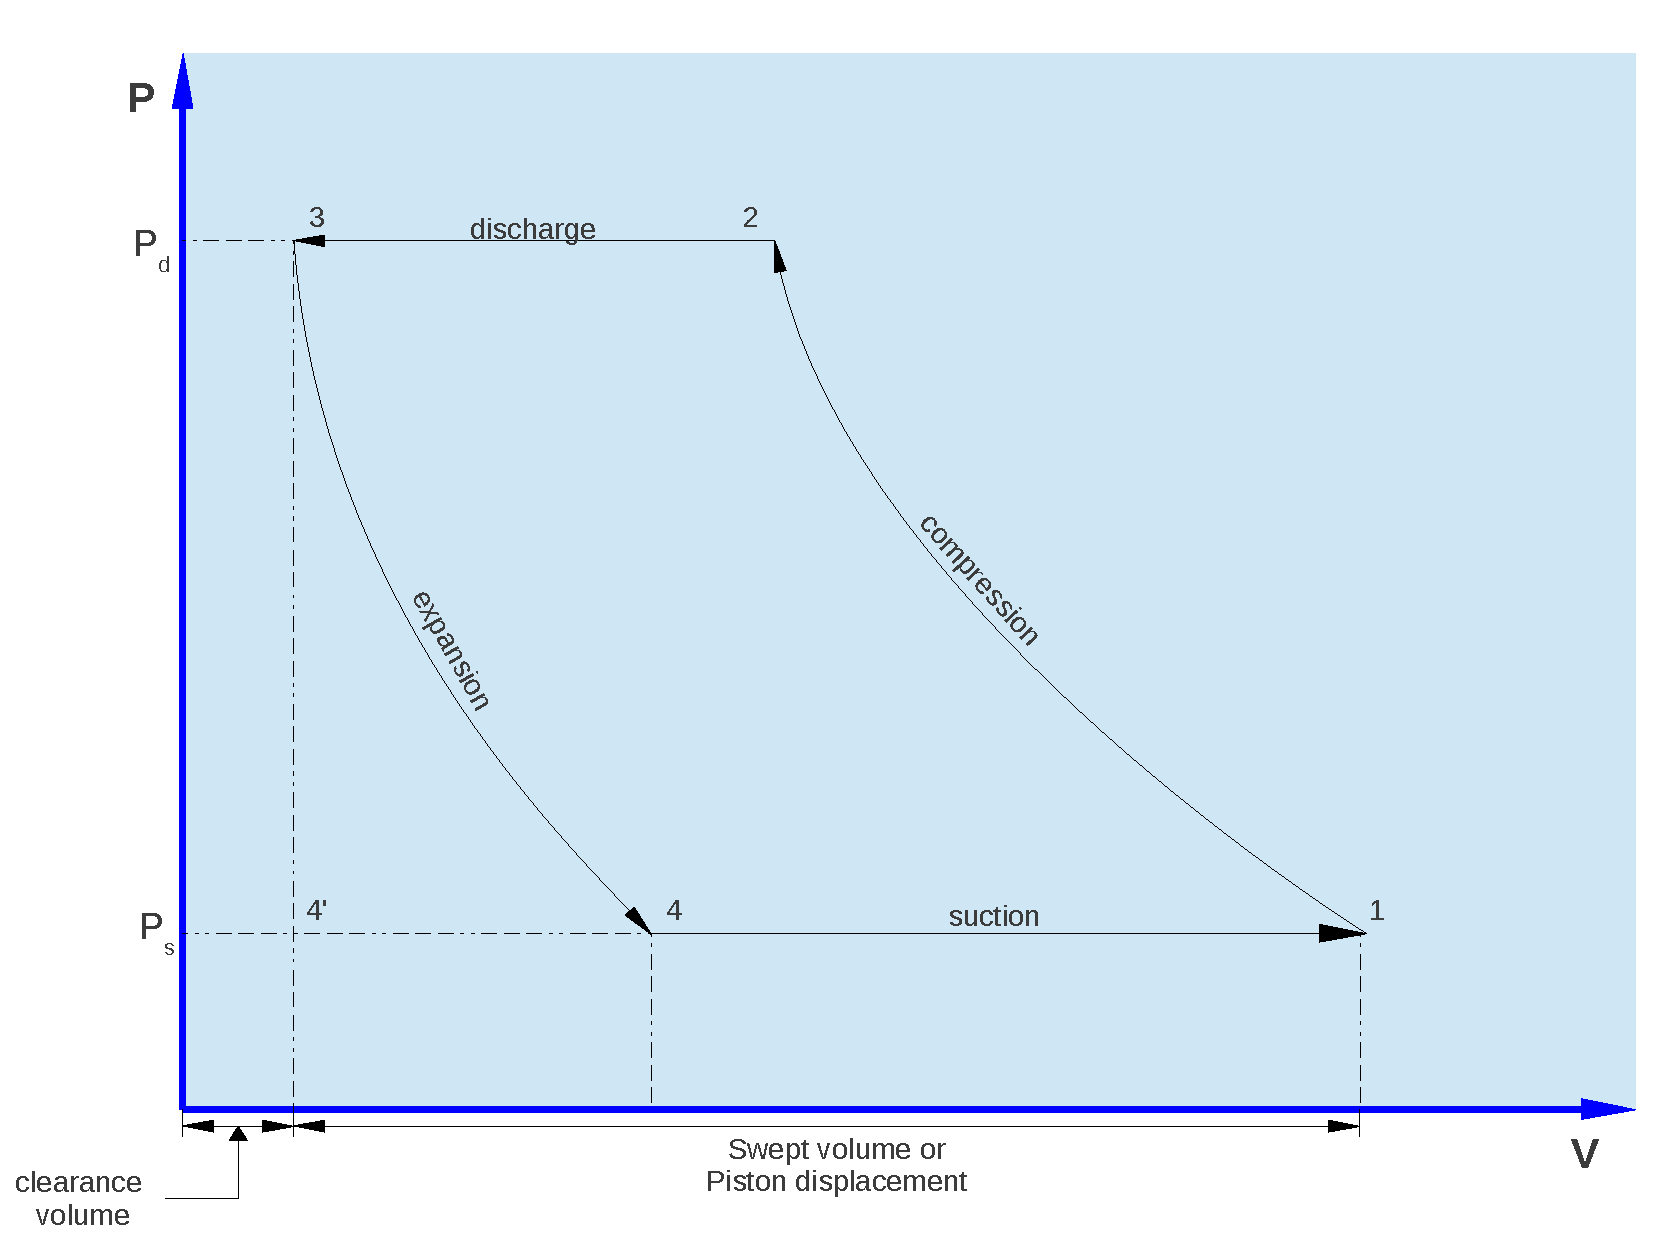
\includegraphics[width=5.cm,height=5.cm,clip]{./Pics/Overview_Refrig29}
    \caption{Clearance volume is the volume of the space between the end of the cylinder and the piston at top dead centre position (TDC).}
   \end{figure}  
  \end{column}  
  \begin{column}[c]{0.55\linewidth}
   \begin{itemize}
    \item <1-> The \textcolor{blue}{Clearance Volumetric Efficiency} with polytropic expansion processes $\left(\text{i.e., }P_{3}V_{3}^{n}=P_{4}V_{4}^{n}\right)$ is defined as 
     \begin{equation}
        \eta_{\text{cv}} = 1 + \mathcal{R}_{c}\left[1-\left(\frc{P_{d}}{P_{s}}\right)^{1/n}\right] \label{clearanceefficiency}
     \end{equation}
    \item <2-> With the clearance ratio,
     \begin{displaymath}
      \mathcal{R}_{c}=\frc{\text{clearance volume}}{\text{swept volume}}=\frc{V_{3}}{V_{1}-V_{3}}
     \end{displaymath}
    \item <3->  See Problem 4 for full derivation of Eqn. \ref{clearanceefficiency}.
    %\item <4->d
   \end{itemize}
  \end{column}  
 \end{columns}
\end{frame}


%%%
%%% Slide
%%%
\begin{frame}
 \frametitle{Thermal Analysis: Volumetric Efficiency of the Compressor}
 \begin{columns}
  \begin{column}[c]{0.35\linewidth}
   \begin{figure}%
      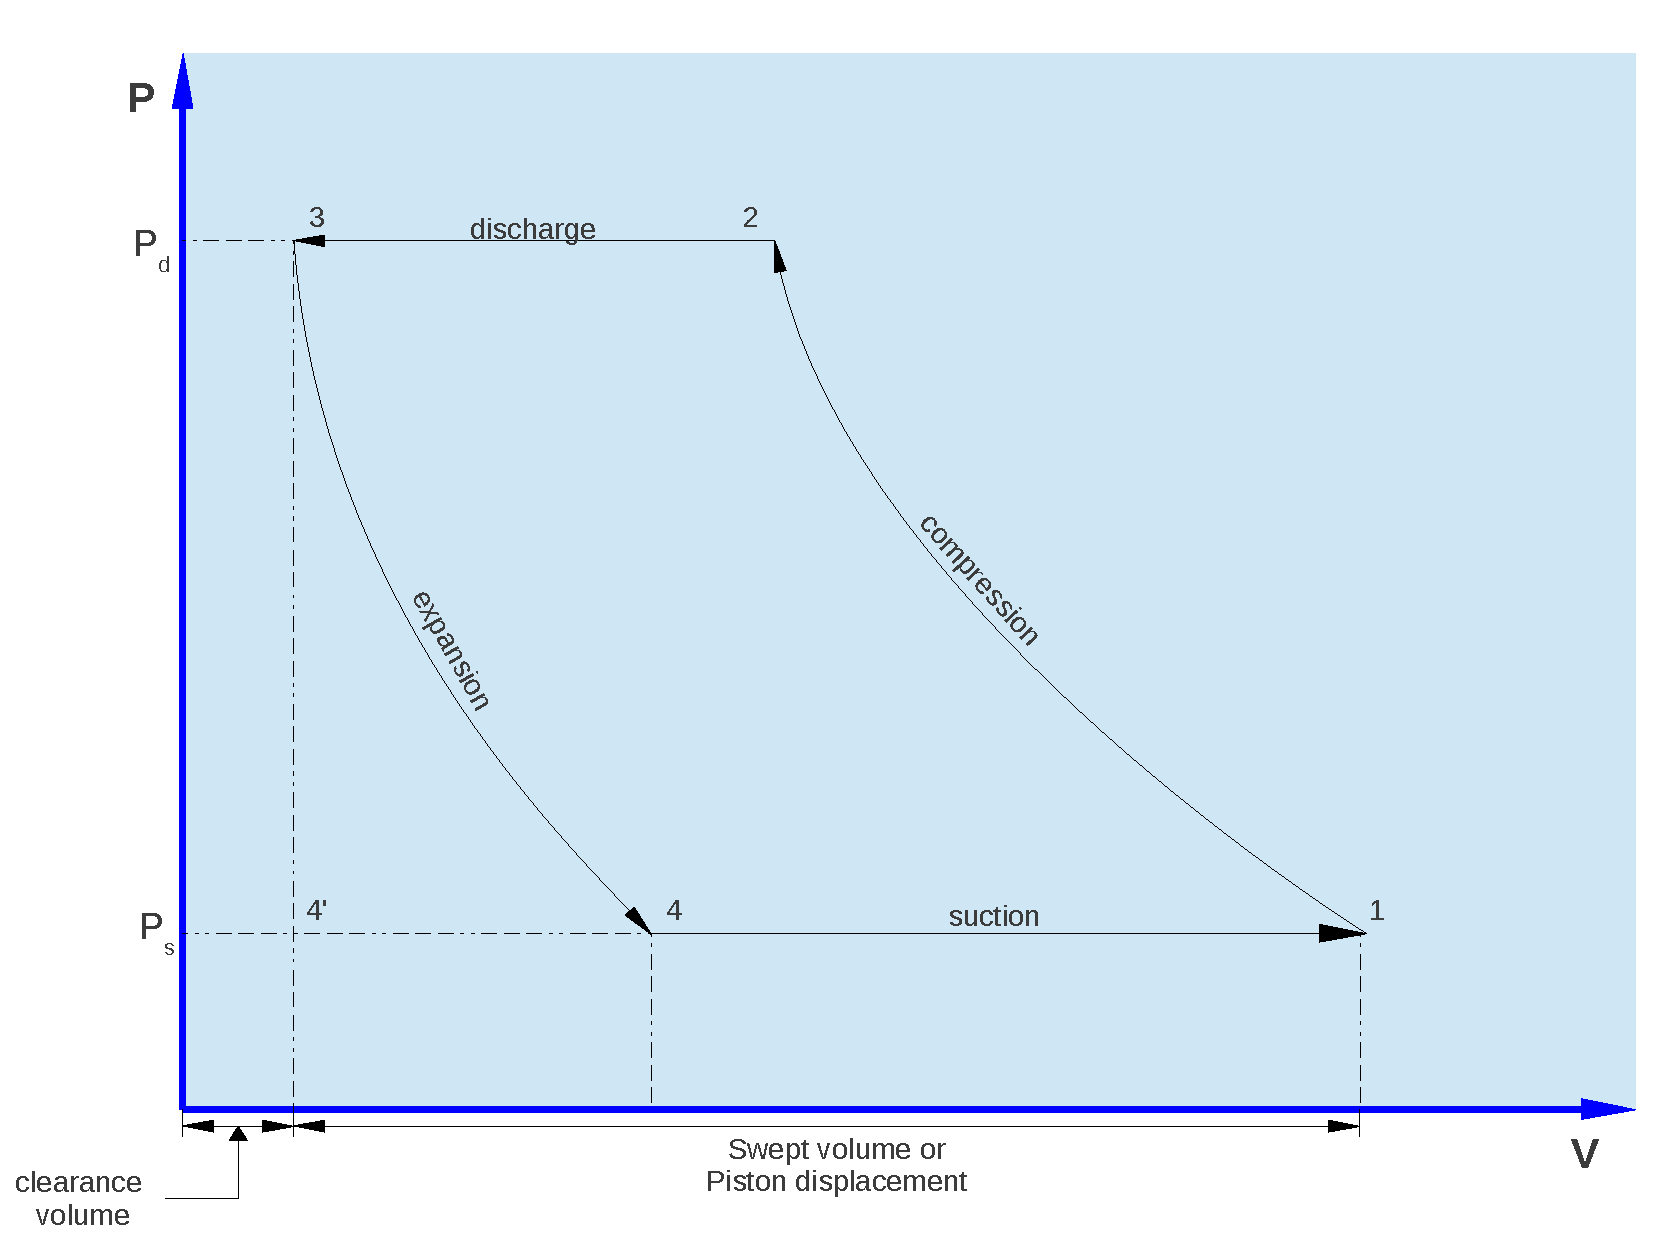
\includegraphics[width=4.5cm,height=4.5cm,clip]{./Pics/Overview_Refrig29}
    %\caption{Clearance volume is the volume of the space between the end of the cylinder and the piston at top dead centre position (TDC).}
   \end{figure}  
  \end{column}  
  \begin{column}[c]{0.65\linewidth}
   \begin{itemize}
    \item <1-> \textcolor{blue}{Total Volumetric Efficiency, $\eta_{V}$} is usually obtained experimentally as it depends on the design of the cycle (e.g., cylinder wall insulation, roughness of the piston-cylinder system and suction line etc);
    \item <2-> It is often calculated from pressure drop measurements in the suction line and the temperature of the gases throughout the suction and expansion strokes,
     \begin{displaymath}
      \textcolor{blue}{\eta_{V} = \left\{1+\mathcal{R}_{c}\left[1-\left(\frc{P_{d}}{P_{s}}\right)^{1/n}\right]\right\} \frc{P_{c}}{P_{s}}\times\frc{T_{s}}{T_{c}}}
     \end{displaymath}
    \item <3-> Where the indeces \textcolor{red}{c} and \textcolor{red}{s} refer to compressor cylinder and evaporator or the suction line adjacent to the compressor.

   \end{itemize}
  \end{column}  
 \end{columns}
\end{frame}


%%%%%%
%%%%%% EXAMPLES
%%%%%%
\begin{frame}
 \frametitle{Example: Single-Stage Vapour-Compression Cycle}
 An ice plant operates on the ideal vapour-compression cycle with superheated state using refrigerant fluid R134a.  The refrigerant enters the compressor as saturated vapour at 0.15 MPa and leaves the condenser as saturated liquid at 0.7 MPa.  Water enters the refrigerator cavity at 30$^{\text{o}}$C and leaves as ice at -5$^{\text{o}}$C. For an ice production rate of 10 kg per hour, determine the power input to the ice plant and the COP of the cycle. Also, sketch the $PH$ and $TS$ diagrams. Specific heats of ice and water are 2.1 and 4.18 kJ/(kg.K), respectively, and the latent heat of fusion of ice is 334 kJ/kg.

\end{frame}

%%%%%%
%%%%%% EXAMPLES
%%%%%%


%%%
%%% Slide
%%%
\begin{frame}
 \frametitle{Multi-Pressure Systems}
 \begin{columns}
  \begin{column}[c]{0.33\linewidth}
   \begin{figure}%
      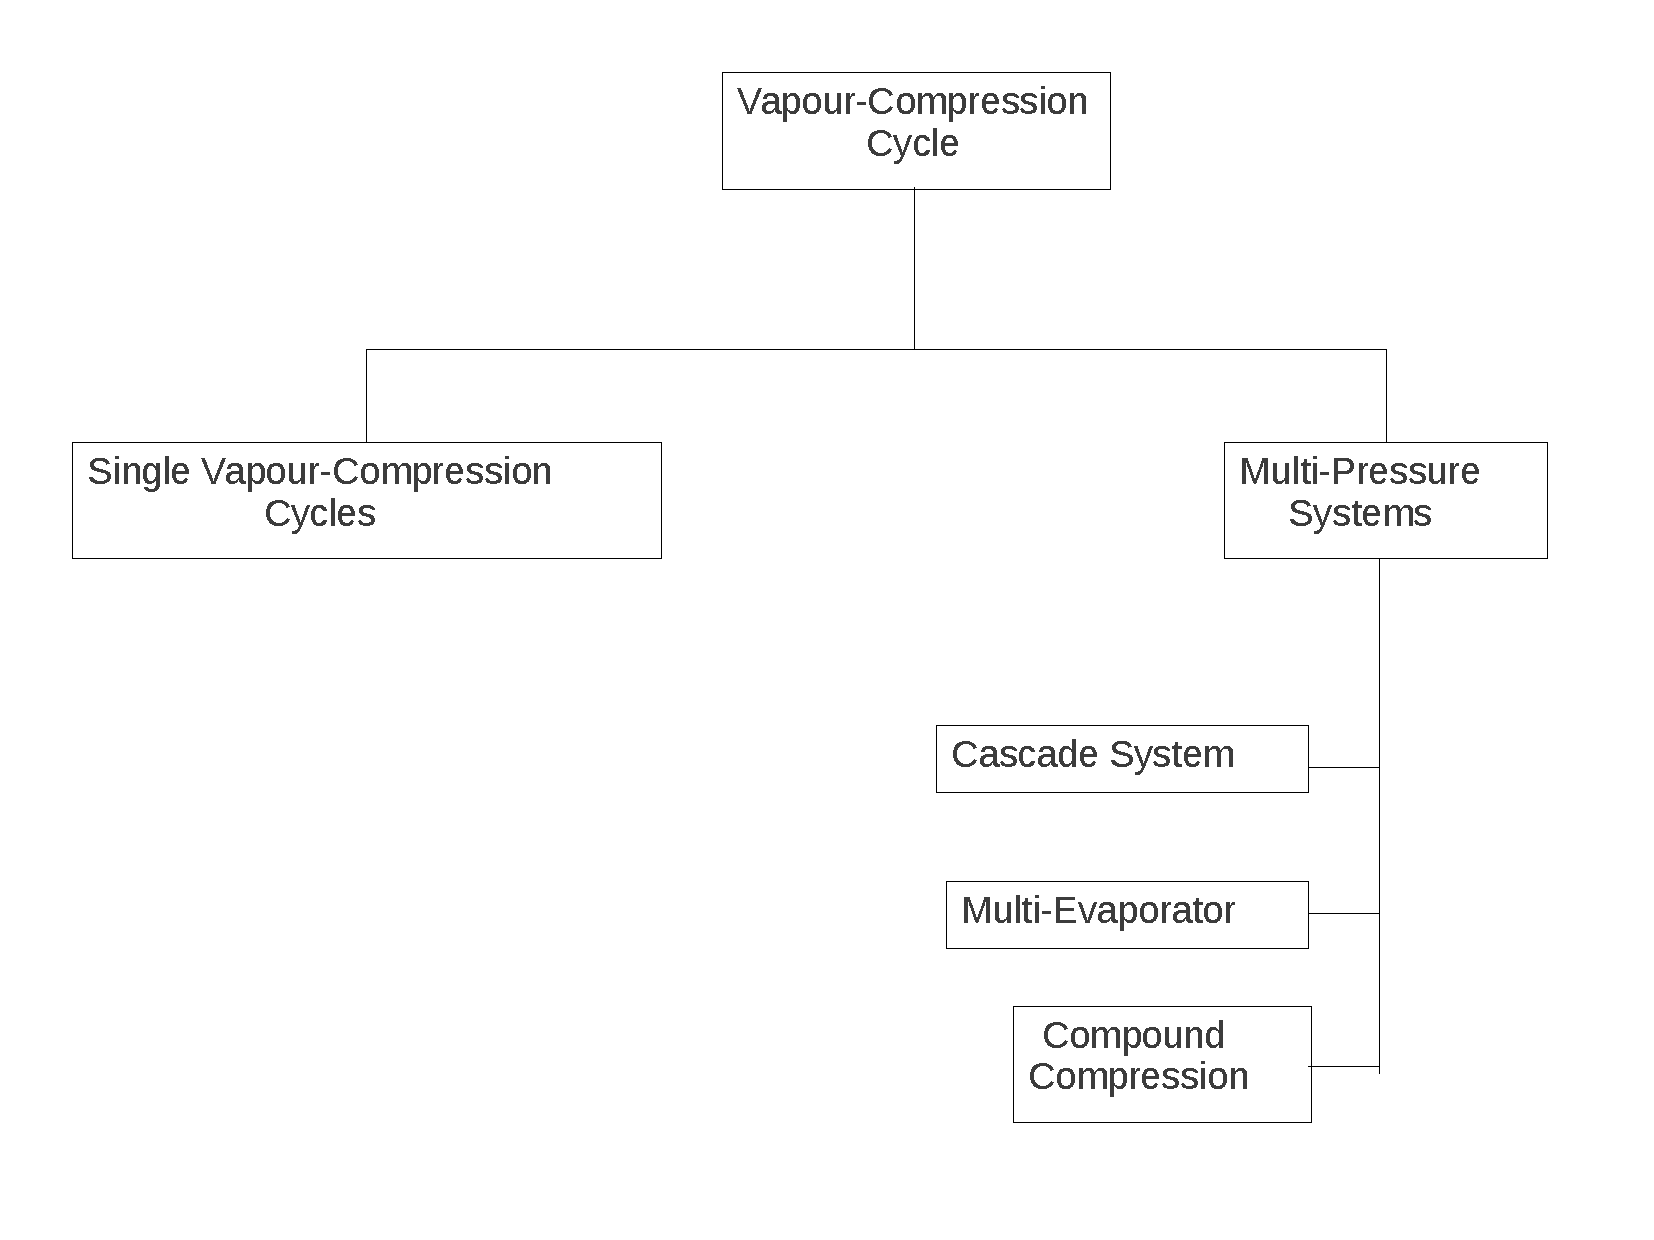
\includegraphics[width=4.5cm,height=4.5cm,clip]{./Pics/Overview_Refrig28}
   \end{figure}  
  \end{column}  
  \begin{column}[c]{0.67\linewidth}
   \begin{enumerate}[(a)]
    \item <1-> Multi-Pressure system is a refrigeration system that has 2 or more pressure levels due to;
    \item <2-> Some industrial processes require 2 or more tempereature levels in the facility. This could be achieved with a set of individual single vapour-compression cycles however;
    \item <3-> The costs associated of such set of cycles may become prohibitive (too costy!);
    \item <4-> For high-condensing and low-evaporating temperature applications, a set of compressors is necessary due to the reduced volumetric efficiency;
    \item <5-> This issue can be overcomed by combining the set of compressors with intercooling;
    \item <6-> While in single-stage compression the lowest working temperature achieved is $\approx$ -30$^{\text{o}}$C, with 2- and 3-stage compression, the temperature may reach -55 and -80$^{\text{o}}$C, respectively.
   \end{enumerate} 
  \end{column}  
 \end{columns} 
\end{frame}


%%%
%%% Slide
%%%
\begin{frame}
 \frametitle{Multi-Stage Cascade Refrigeration}
 \begin{columns}
  \begin{column}[c]{0.45\linewidth}
   \begin{figure}%
     \vbox{
      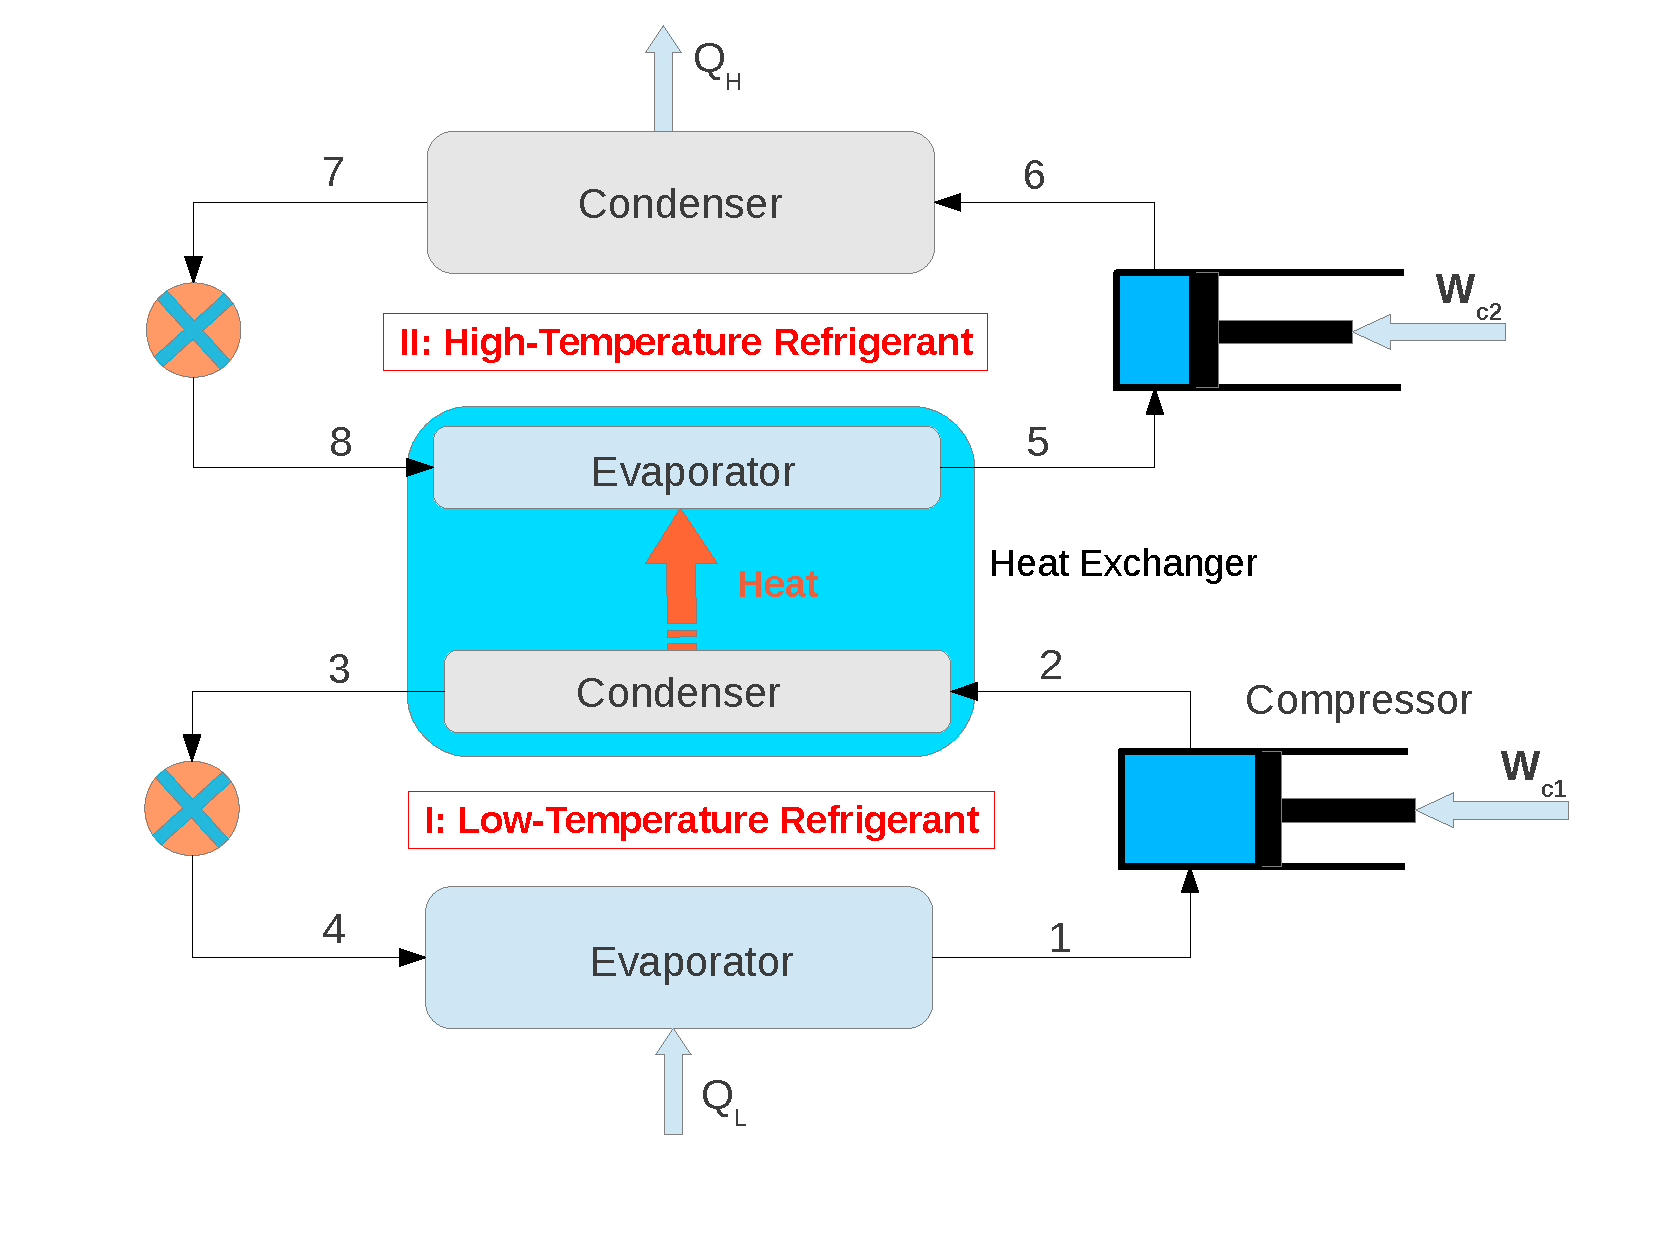
\includegraphics[width=4.5cm,height=3.5cm,clip]{./Pics/Overview_Refrig24}
      \vspace{-.1cm}
      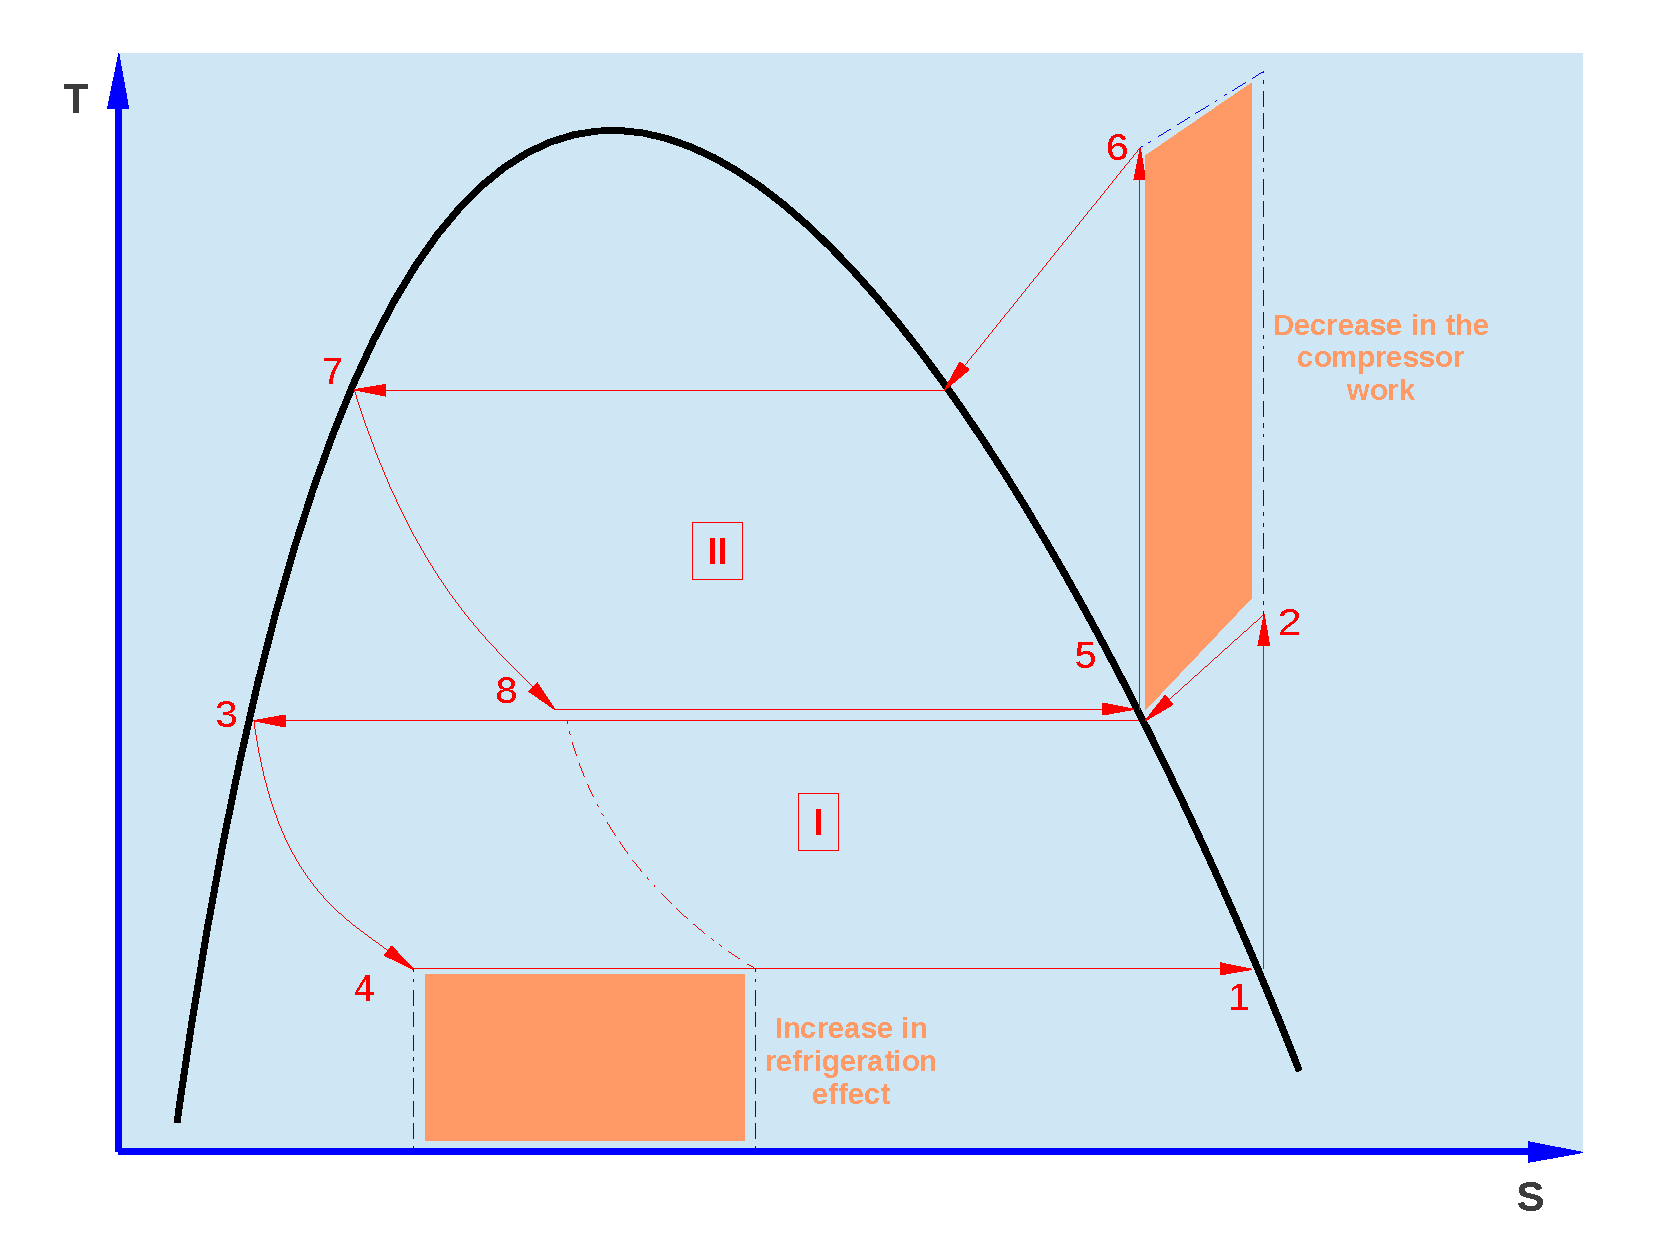
\includegraphics[width=4.cm,height=4.cm,clip]{./Pics/Overview_Refrig25}}
   \end{figure}  
  \end{column}  
  \begin{column}[c]{0.55\linewidth}
   \begin{enumerate}[(a)]
    \item <1-> Simple vapour-compression refrigeration cycles are inexpensive and reliable however for large industrial systems \textcolor{blue}{efficiency} is a major requirement;
    \item <2-> Some industrial applications requires large temperature range which leads to large pressure range (and therefore low performance/efficiency in the compressor);
    \item <3-> Similar to the vapour thermal systems, we can improve the efficiency of the cycle by coupling two (or more) cycles (in parallel) through heat exchangers that will operate simultaneously as evaporator and condenser;
   \end{enumerate} 
  \end{column}  
 \end{columns} 
\end{frame}


%%%
%%% Slide
%%%
\begin{frame}
 \frametitle{Multi-Stage Cascade Refrigeration}
 \begin{columns}
  \begin{column}[c]{0.35\linewidth}
   \begin{figure}%
     \vbox{
      \includegraphics[width=4.5cm,height=3.5cm,clip]{./Pics/Overview_Refrig24}
      \vspace{-.1cm}
      \includegraphics[width=4.cm,height=4.cm,clip]{./Pics/Overview_Refrig25}}
   \end{figure}  
  \end{column}  
  \begin{column}[c]{0.65\linewidth}
   \begin{enumerate}[(a)]
    \item <1-> If we assume that there is no heat loss to the surrounding, cycles \textcolor{red}{I} and \textcolor{red}{II} can be related by the mass flow rates in the heat exchanger:
      \begin{displaymath}
       \dot{m}_{I}\left(H_{2}-H_{3}\right)=\dot{m}_{II}\left(H_{5}-H_{8}\right)\Rightarrow \frc{\dot{m}_{I}}{\dot{m}_{II}}=\frc{H_{5}-H_{8}}{H_{2}-H_{3}}
      \end{displaymath}
    \item <2-> And the COP is defined as
     \begin{eqnarray}
      \text{COP}= \frc{Q_{L}}{\sum\limits_{i=1}^{2}W_{c,i}} = \frc{\dot{m}_{I}\left(H_{1}-H_{4}\right)}{\dot{m}_{II}\left(H_{6}-H_{5}\right)+\dot{m}_{I}\left(H_{2}-H_{1}\right)}\nonumber\\
            \;\;\;\;\;= \frc{\left(H_{5}-H_{8}\right)\left(H_{1}-H_{4}\right)}{\left(H_{6}-H_{5}\right)\left(H_{2}-H_{3}\right)+\left(H_{5}-H_{8}\right)\left(H_{2}-H_{1}\right)}
     \end{eqnarray}
   \end{enumerate}
  \end{column}  
 \end{columns} 
\end{frame}



%%%
%%% Slide
%%%
\begin{frame}
 \frametitle{Multi-Stage Cascade Refrigeration}
 \begin{columns}
  \begin{column}[c]{0.45\linewidth}
   \begin{figure}%
     \vbox{
      \includegraphics[width=4.5cm,height=3.5cm,clip]{./Pics/Overview_Refrig24}
      \vspace{-.1cm}
      \includegraphics[width=4.cm,height=4.cm,clip]{./Pics/Overview_Refrig25}}
   \end{figure}  
  \end{column}  
  \begin{column}[c]{0.55\linewidth}
   \begin{enumerate}[(a)]
    \item <1-> The number of stages depends only on the required temperature range;
    \item <2-> The refrigerant fluid will also depend upon the required temperature and thus 2 or more fluids can be used as they do not mix (i.e., mass-isolated cycles).
   \end{enumerate}
  \end{column}  
 \end{columns} 
\end{frame}


%%%
%%% Slide
%%%
\begin{frame}
 \frametitle{Multi-Stage Compression with Intercooling Refrigeration}
 \begin{columns}
  \begin{column}[c]{0.45\linewidth}
   \begin{figure}%
     \vbox{
      \includegraphics[width=4.5cm,height=3.5cm,clip]{./Pics/Overview_Refrig26}
      \vspace{-.1cm}
      \includegraphics[width=4.cm,height=4.cm,clip]{./Pics/Overview_Refrig27}}
   \end{figure}  
  \end{column}  
  \begin{column}[c]{0.55\linewidth}
   \begin{enumerate}[(a)]
    \item <1-> This special and complex process is applied when the cascade refrigeration is used with \textcolor{blue}{a single refrigerant fluid};
    \item <2-> In this case, the heat exchanger is replaced by a \textcolor{blue}{{\it flash chamber}} (i.e., a liquid-vapour separator);
    \item <3-> The refrigerant is partially compressed in the LP stage (1-2);
    \item <4-> After leaving the LP compressor, the fluid is cooled by mixing with vapour stream from the flash chamber (3) in the intermediate heat exchanger to a temperature $T_{9}<T_{2}$;
    \item <5-> Such reduction of temperature results in smaller compressor work.
   \end{enumerate}
  \end{column}  
 \end{columns} 
\end{frame}


%%%
%%% Slide
%%%
\begin{frame}
 \frametitle{Multi-Stage Compression with Intercooling Refrigeration}
 \begin{columns}
  \begin{column}[c]{0.45\linewidth}
   \begin{figure}%
     \vbox{
      \includegraphics[width=4.5cm,height=3.5cm,clip]{./Pics/Overview_Refrig26}
      \vspace{-.1cm}
      \includegraphics[width=4.cm,height=4.cm,clip]{./Pics/Overview_Refrig27}}
   \end{figure}  
  \end{column}  
  \begin{column}[c]{0.55\linewidth}
   \begin{enumerate}[(a)]
    \item <1-> The fluid is then compressed in the HP (stage 4) and driven to the condenser where it becomes a saturated liquid;
    \item <2-> The liquid refrigerant is expanded (5-6) until the pressure is reduced to the interstage pressure and sent to the flash chamber;
    \item <3-> The liquid-vapour solution (2-phase region) from the condenser is separated (in the flash chamber) and;
    \item <4-> The liquid fraction is driven to the second expansion valve (7-8) where;
    \item <5-> The refrigerant pressure is reduced and the fluid is driven to the evaporator (8-1) where;
   \end{enumerate}
  \end{column}  
 \end{columns} 
\end{frame}


%%%
%%% Slide
%%%
\begin{frame}
 \frametitle{Multi-Stage Compression with Intercooling Refrigeration}
 \begin{columns}
  \begin{column}[c]{0.45\linewidth}
   \begin{figure}%
     \vbox{
      \includegraphics[width=4.5cm,height=3.5cm,clip]{./Pics/Overview_Refrig26}
      \vspace{-.1cm}
      \includegraphics[width=4.cm,height=4.cm,clip]{./Pics/Overview_Refrig27}}
   \end{figure}  
  \end{column}  
  \begin{column}[c]{0.55\linewidth}
   \begin{enumerate}[(a)]
    \item <1-> The liquid refrigerant is vaporised  by absorbing latent heat of vaporisation from the refrigerated space (cooling effect);
    \item <2-> The gas fraction (3) enters the heat exchange and is mixed with the fluid leaving the first LP compressor and driven to the HP compressor (9-4).
    \item <3-> For two-stage compression of a refrigerant with complete intercooling, for minimum work, the interstage pressure, $P_{i}$ is approximate to,
      \begin{displaymath}
       P_{i}=\sqrt{P_{1}P_{2}}
      \end{displaymath}
    \item <4-> Where $P_{1}$ is the suction pressure of the LP compressor and $P_{2}$ is the discharge pressure of the HP compressor.
   \end{enumerate}
  \end{column}  
 \end{columns} 
\end{frame}



%%%
%%% Slide
%%%
\begin{frame}
 \frametitle{Example: Multi-Stage Compression with Intercooling Refrigeration}
 \begin{columns}
  \begin{column}[c]{0.45\linewidth}
   \begin{figure}%
      \includegraphics[width=5.5cm,height=4.5cm,clip]{./Pics/Overview_Refrig30}
   \end{figure}  
  \end{column}  
  \begin{column}[c]{0.55\linewidth}
   An ammonia refrigeration system, the evaporator supplies 300kW of refrigeration at -30$^{\text{o}}$C.  The system uses 2-stage compression as shown in the Figure, with intercooling and removal of flash gas.  The condensing temperature is 35$^{\text{o}}$C.
    \begin{enumerate}[(a)]
     \item Sketch the $PH$ diagram;
     \item Calculate the power required by the compressors;
     \item Determine the coefficient of performance.
    \end{enumerate}

Assume that the intermediate pressure is expressed as: $P_{i}=\sqrt{P_{5}P_{1}}$.
  \end{column}  
 \end{columns} 
\end{frame}





\section{Summary}

%%%
%%% Slides
%%%
\begin{frame}
 \frametitle{Summary}
  After this lecture you should:
 \begin{enumerate}[(a)]
  \item <1-> Identify elements of the vapour-compressed refrigeration systems;
  \item <2-> Link the thermo-fluid dynamics learnt in Module 3 with the use of expansion valves in Module 4;
  \item <3-> Be able to sketch $PH$ and $TS$ diagrams and perform a thermal analysis of the cycles.
 \end{enumerate}
\end{frame}



\end{document}
